% Author :  Lionel du Peloux
% Contact : lionel.dupeloux@gmail
% Year : 2017

\chapter{Elastic gridshells}
%
%\cite{Barnes1975}
%\citeauthor{Barnes1975}
%\cite{Bouhaya2009}
%\citeauthor{Bouhaya2009}
%\citetitle{Bouhaya2009}
%\cite{ALCIMED2012}

\section{Elastic gridshells : a review}

\blockcquote[][p.~2]{Harris2003}{Ted Happold (1930–96), founding partner of Buro Happold, worked on the Mannheim gridshell in Germany (Architect Frei Otto, built 1975), when he was with Ove Arup \& Partners. For many years after its completion, Happold promoted the benefit of the timber gridshell as a construction technique and stated that he could not understand why it had not been adopted more widely. He perceived the benefits to be in the efficiency of the construction method to enable doubly curved (shell) structures to be constructed quickly and cost effectively. A doubly curved structure offers the benefits of a minimal use of materials and therefore an efficient coverage of space. Such a structure can be made either in situ in the case of concrete or in a factory in the case of steel or aluminium. Except in the case of a spherical gridshell, the repetition of the ele- ments is very limited and the shell is made from a com- plex set of components. In contrast, a timber gridshell enables doubly curved structures to be formed from a set of straight, prefabricated, identical components. A number of Happold’s partners at Buro Happold had worked with him on the Mannheim gridshell and, when the opportunity arose to design a series of small land- scape structures at the Earth Centre, near Doncaster, UK, in 1994, gridshells were proposed.}

\blockcquote[][p.~2]{Harris2003}{The key to the modern use of timber gridshells is the development of computer methods in modelling complex three-dimensional shell structures. }

\blockcquote[][p.~250]{IL10}{At present, the architectural significance of grid shells can hardly be fully envisioned. Too little experience has been gained as yet. However, the first signs of a grid shell architecture are already apparent. The projects planned and executed to date and the results of this research work indicate possibilities that open up a wide field of applications for grid shells. Two things stand out above all. The first is the nearly unlimited variety of forms that can be realized with grid shells, the second is the fact that there is no closed shell surface, but rather a simple, spatially curved grid composed of rods. Both features are of fundamental significance. They fully characterize the architectural essence of the grid shell support structure.}

\blockcquote[][p.~179]{IL10}{From the inverted form to the gridshell}

\clearpage

\clearpage

\subsubsection{The beginnings : from the first prototype to the German Pavilion}

Frei Otto started his studies in architecture in 1947 in Berlin, Germany, and completed his doctorate on tensile structures in 1953. This first work was published and translated later in the 60's. He then began to work in the field of lightweight structures using physical models such as soap films or hanging nets, and photographic measurements.\footnote{In the 19\textsuperscript{th} and 20\textsuperscript{th} centuries model testing was at the heart of structural innovation \cite{Addis2013}. Analog models were employed successfully by well-known architects and engineers to go beyond the limits of existing knowledge (A. Gaudi, H. Isler, F. Candela, F. Otto, \telp{}) and are still employed today where numeric models failed to represent accurately some physical phenomenons (for instance in wind analysis for high rise towers and bridges).}\textsuperscript{,}\footnote{\blockcquote[p.~56]{IL10}{Photography is the medium through which the form and content of a model are communicated. It is one of our most important tools in that it provides the basis for documentation and information, supplements our creative potential \belp{} }} These tools were essentials for his exploration of forms and structures as there were no computers at that time.

Simultaneously, he became interested by the study of lightweight shells and the way they were form-found. One of his very first elastic gridshell was built in 1962 with students at Berkeley, USA \cite[p.~270]{IL10}. It is funny to remark that this first gridshell was not a timber gridshell but a steel gridshell made out of twin steel rods linked in a grid fashion by bolts with clamping plates. This first experiment demonstrated at small scale the ability to bend a regular grid with no shear rigidity into a curved shape. The grid was loosely braced and shell effects were not investigated.
\begin{figure}[ht]
		\subfloat[][Knot detail]{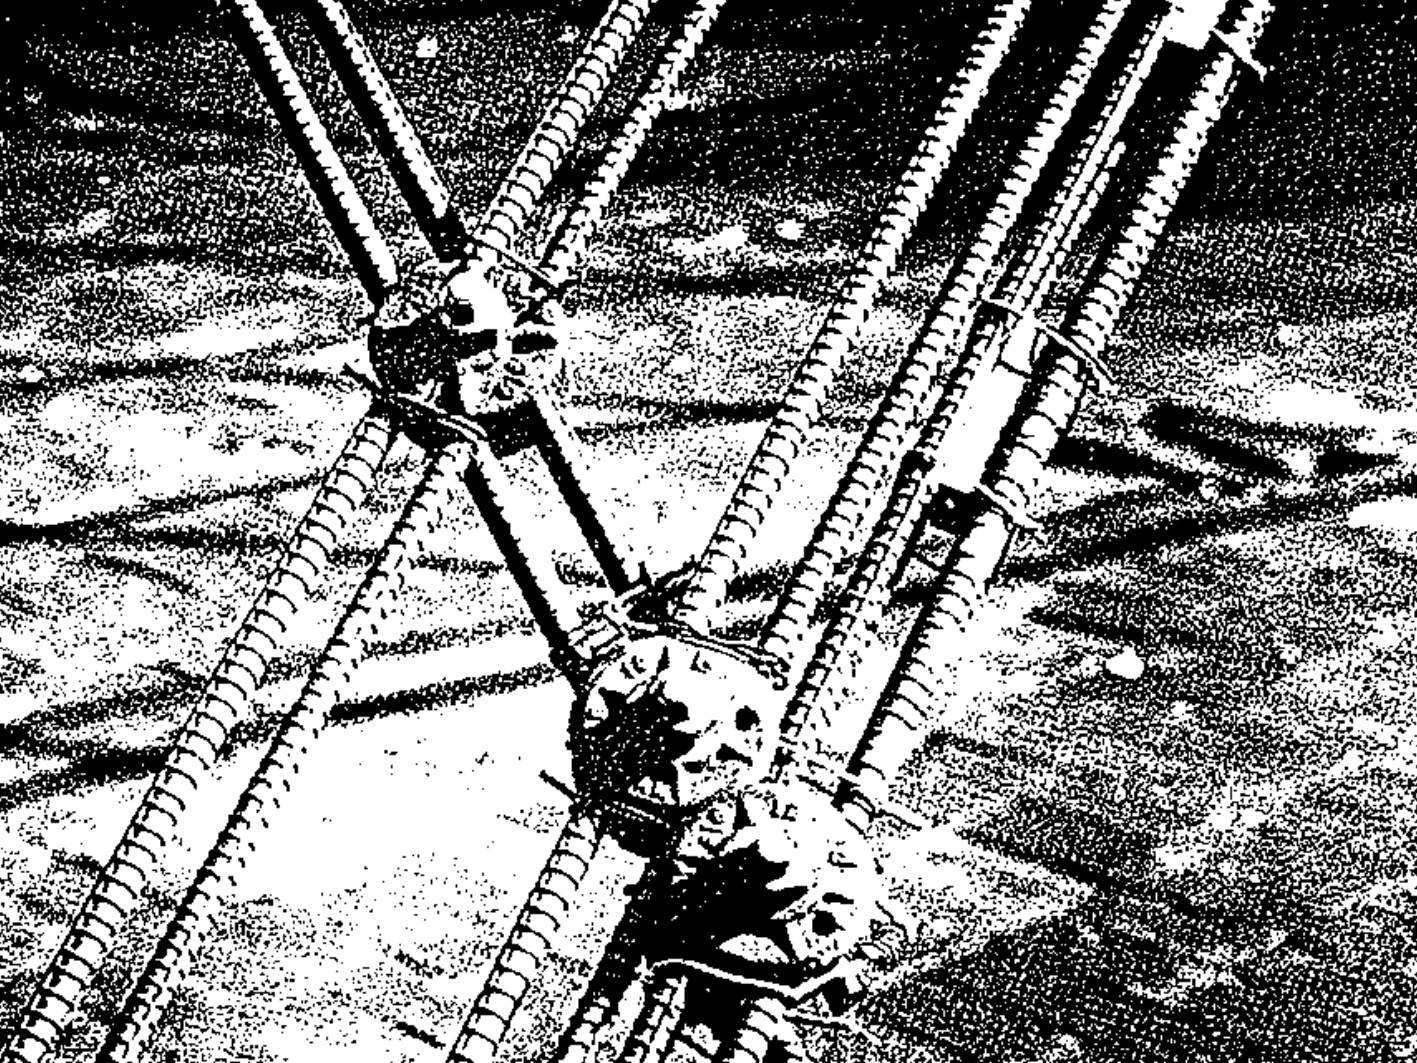
\includegraphics[width=0.48\textwidth]{berkeley_detail.jpg}\label{fig:berkeley_a}}
		\hspace*{\fill}
		\subfloat[][Steel lattice]{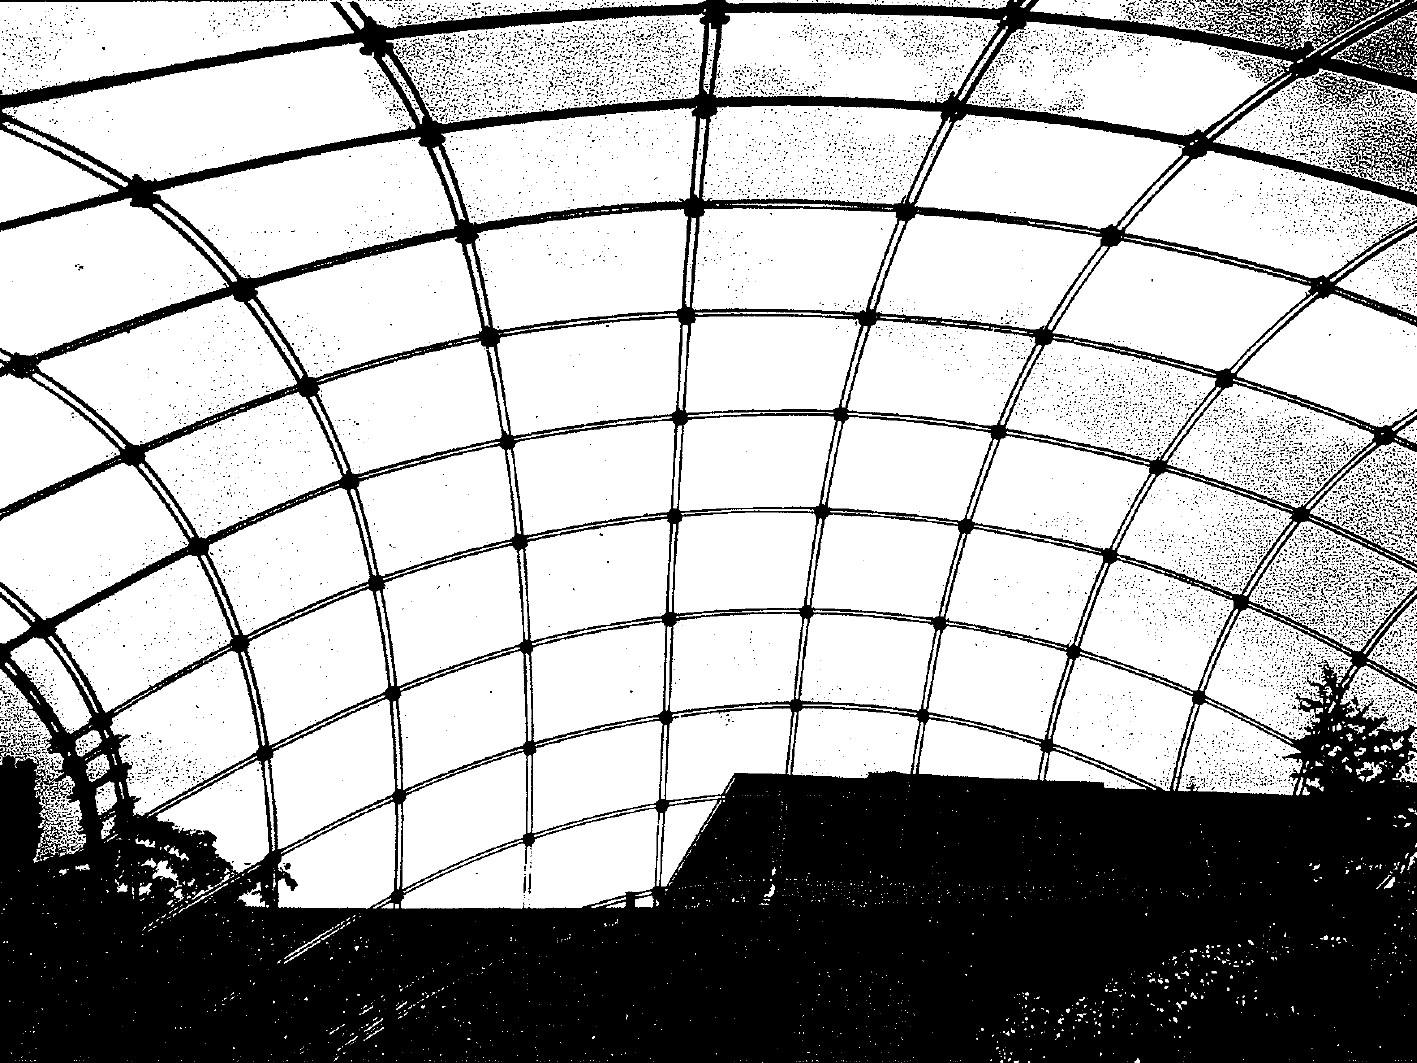
\includegraphics[width=0.48\textwidth]{berkeley_gs.jpg}\label{fig:berkeley_b}}
		%
		\vspace{10pt}
		\caption{Steel gridshell built in Berkeley, USA, in 1962.}
		\label{fig:berkeley}    
\end{figure}
The same year he designed and built a first timber gridshell at Essen, Germany \cite[p.~272]{IL10}. The prototype~-- a single layer gridshell spanning \SI{17}{m} and covering an area of \SI{198}{m^2} -- was made with 3-plies laminated timber profiles in hemlock pine. The cross-section of the profiles was rectangular (\SI{60}{mm} x \SI{40}{mm}) and the elements were assembled in a grid fashion with simple steel bolts. Once erected, nothing was specifically done to improve the in-plane shear stiffness of the grid and activate a shell behavior. Finally, the structure was covered with a transparent plastic foil nailed directly on the grid's profiles.
\begin{figure}[t]
		\subfloat[][Timber lattice]{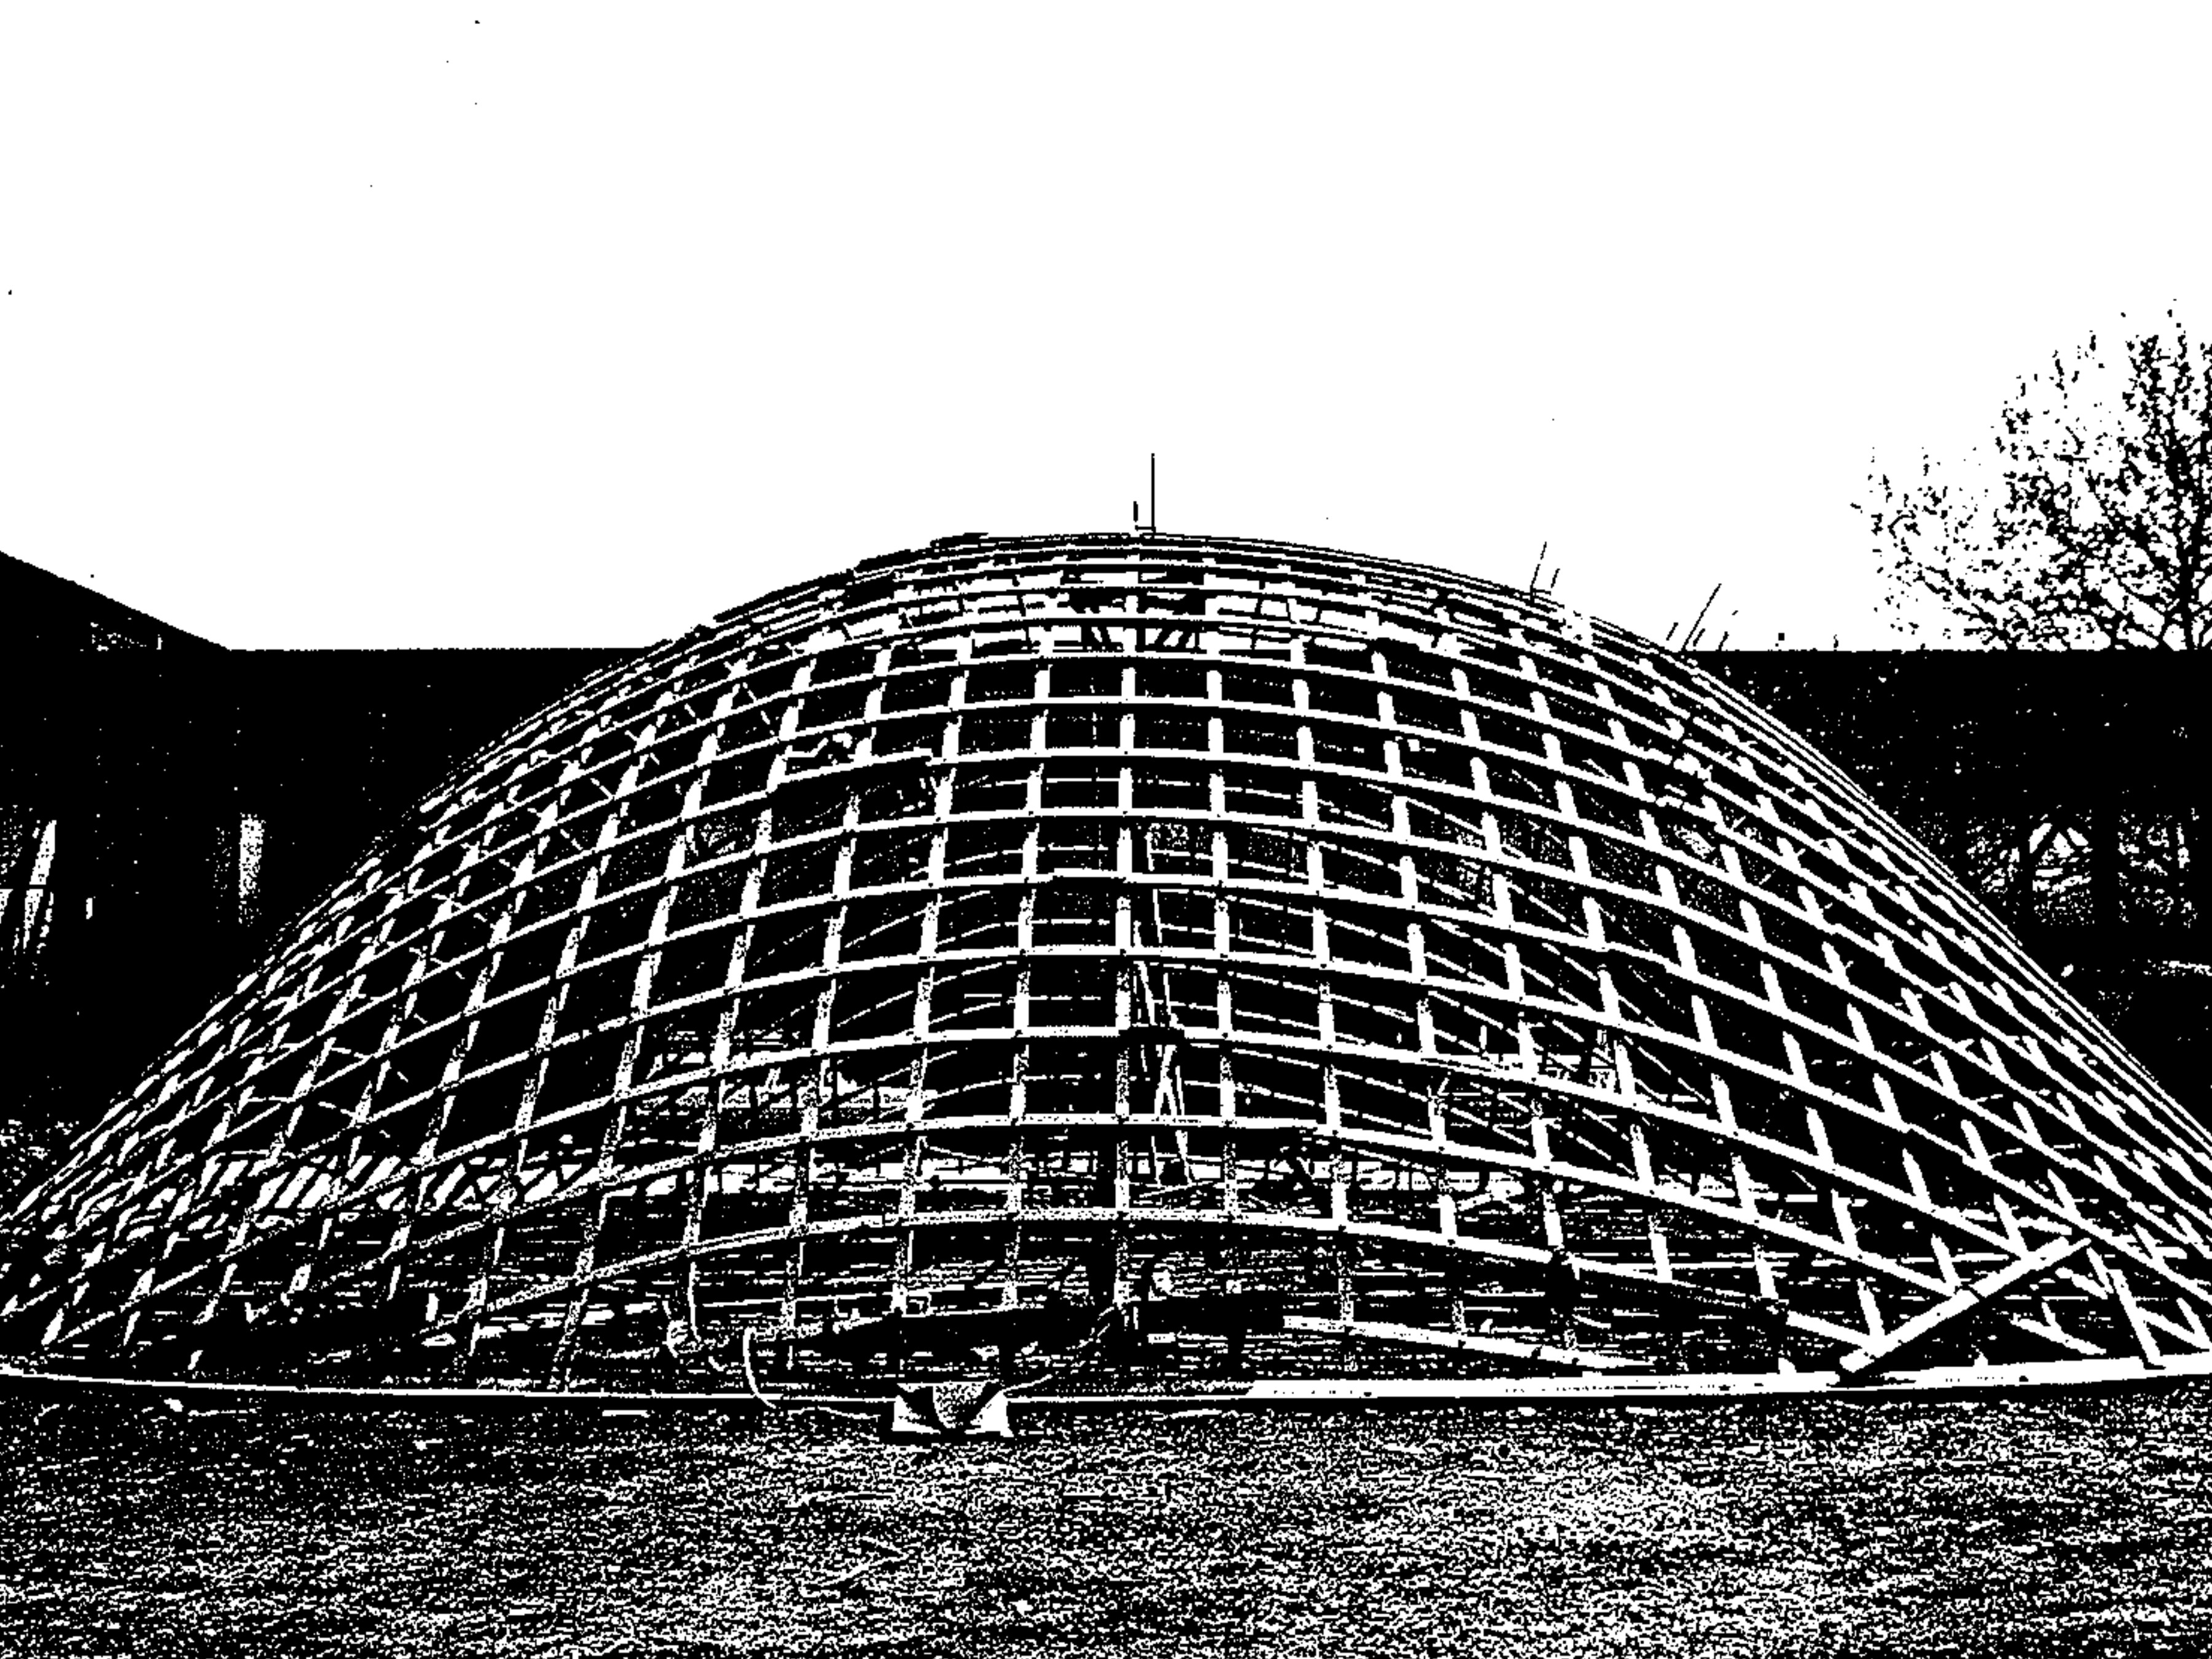
\includegraphics[width=0.48\textwidth]{essen_gs.jpg}\label{fig:essen_a}}
		\hspace*{\fill}
		\subfloat[][Plastic foil]{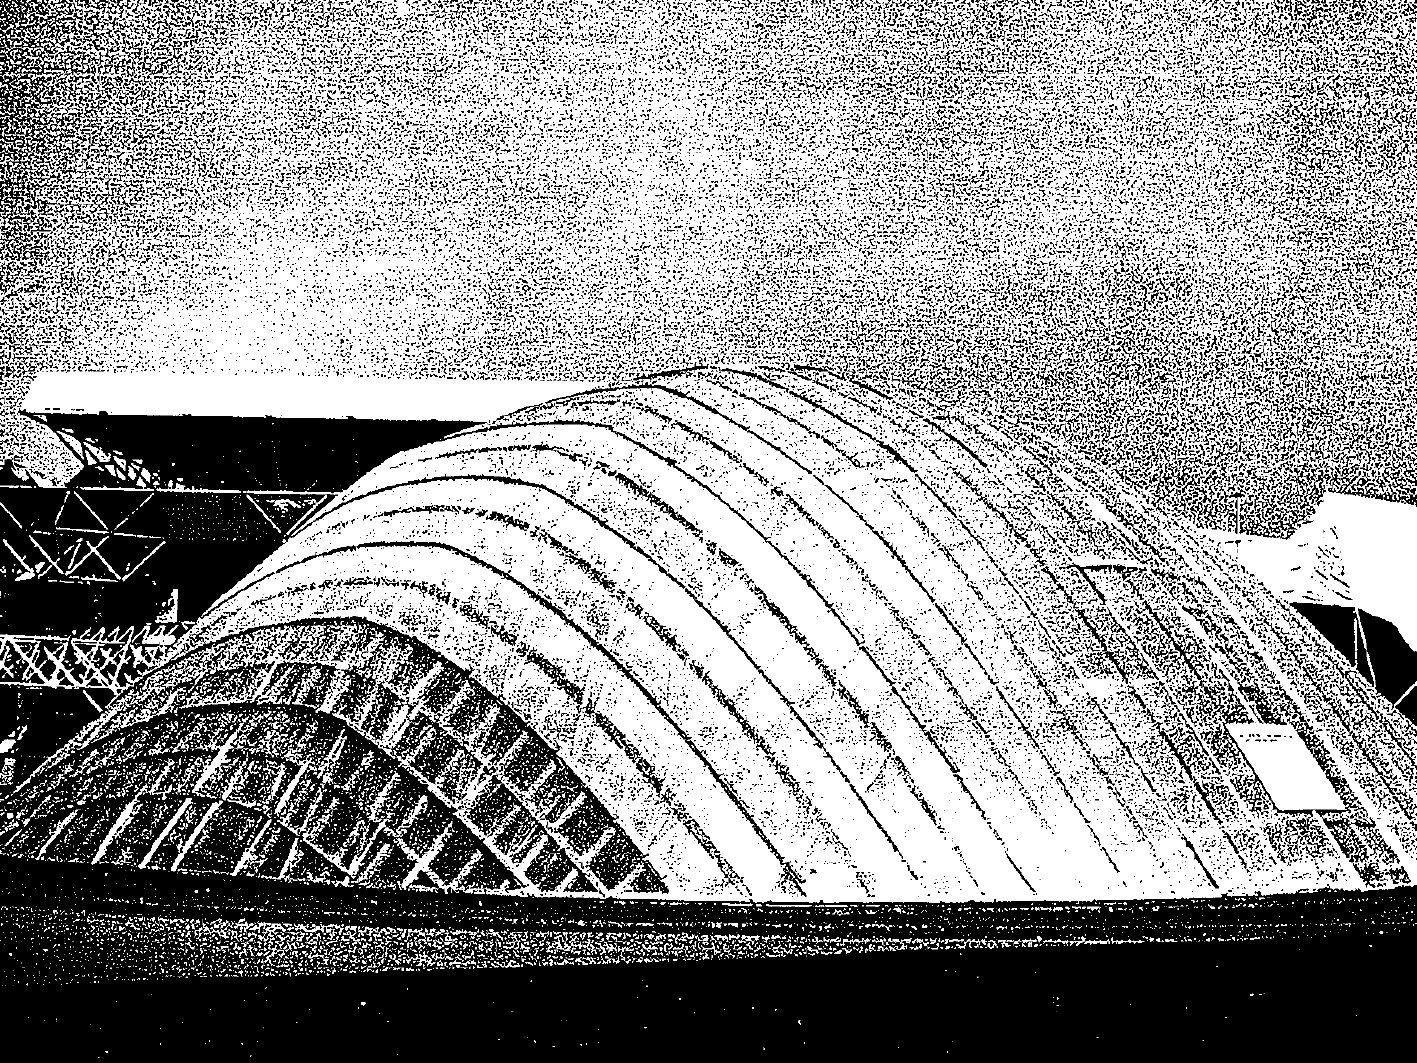
\includegraphics[width=0.48\textwidth]{essen_foil.jpg}\label{fig:essen_b}}
		%
		\vspace{10pt}
		\caption{Timber gridshell built in 1962 in Essen, Germany.}
		\label{fig:essen}    
\end{figure}
Fiver years later, on the occasion of the \emph{1967 International and Universal Exposition} in Montreal, Canada, Frei Otto was appointed to design the German Pavilion~: a large cable net tent prefiguring the realization of the olympic stadium of Munich, Germany, in 1972.\footnote{Actually, Frei Otto became the director of the newly founded \emph{Institute for Lightweight Structures} (Institut für Leichte Flächentragwerke or IL) at the University of Stuttgart in 1964. It was the IL that was commissioned by the German government to conduct research in connection with the planning of the German pavilion for the exposition in Montreal} The pavilion required two auditoria and these were designed using the principle of elastic gridshell \cite[p.~274]{IL10}. All together, the auditoria covered and area of \SI{365}{m^2} and spanned \SI{17.5}{m}. The construction technic employed in Montreal was quite similar to the one developed in Essen, but this time the grid was fully braced with a layer of nailed plywood boards and offered a proper roofing made out of insulation panels covered with a PVC coated fabric.

The two gridshells built in Montreal mark a significant step in the maturation process of the technic leading to the major realization of Mannheim in 1976~: a methodology has emerged to progress \blockcquote[p.~179]{IL10}{from the inverted form to the gridshell} ; main construction details have been validated ; various erection methods have been tested ; mid-scale buildings have been built to host public. However, due to the over complexity of these structures, lots of unknowns remained unsolved at this stage and the behavior of the structures could not be fully predicted.\footnote{\blockcquote[p.~219]{IL10}{Snow accumulations in the throat of the common edge beam probably caused one of the two grid shells of project Montreal to buckle in a relatively flat region. The diameter of the buckled area was about 3 meters. Neither grid rod was broken, i.e. the buckling progressed elastically. It might have been possible to press the buckled area back into shape.}}
\begin{figure}[H]
		\subfloat[][Grid erection]{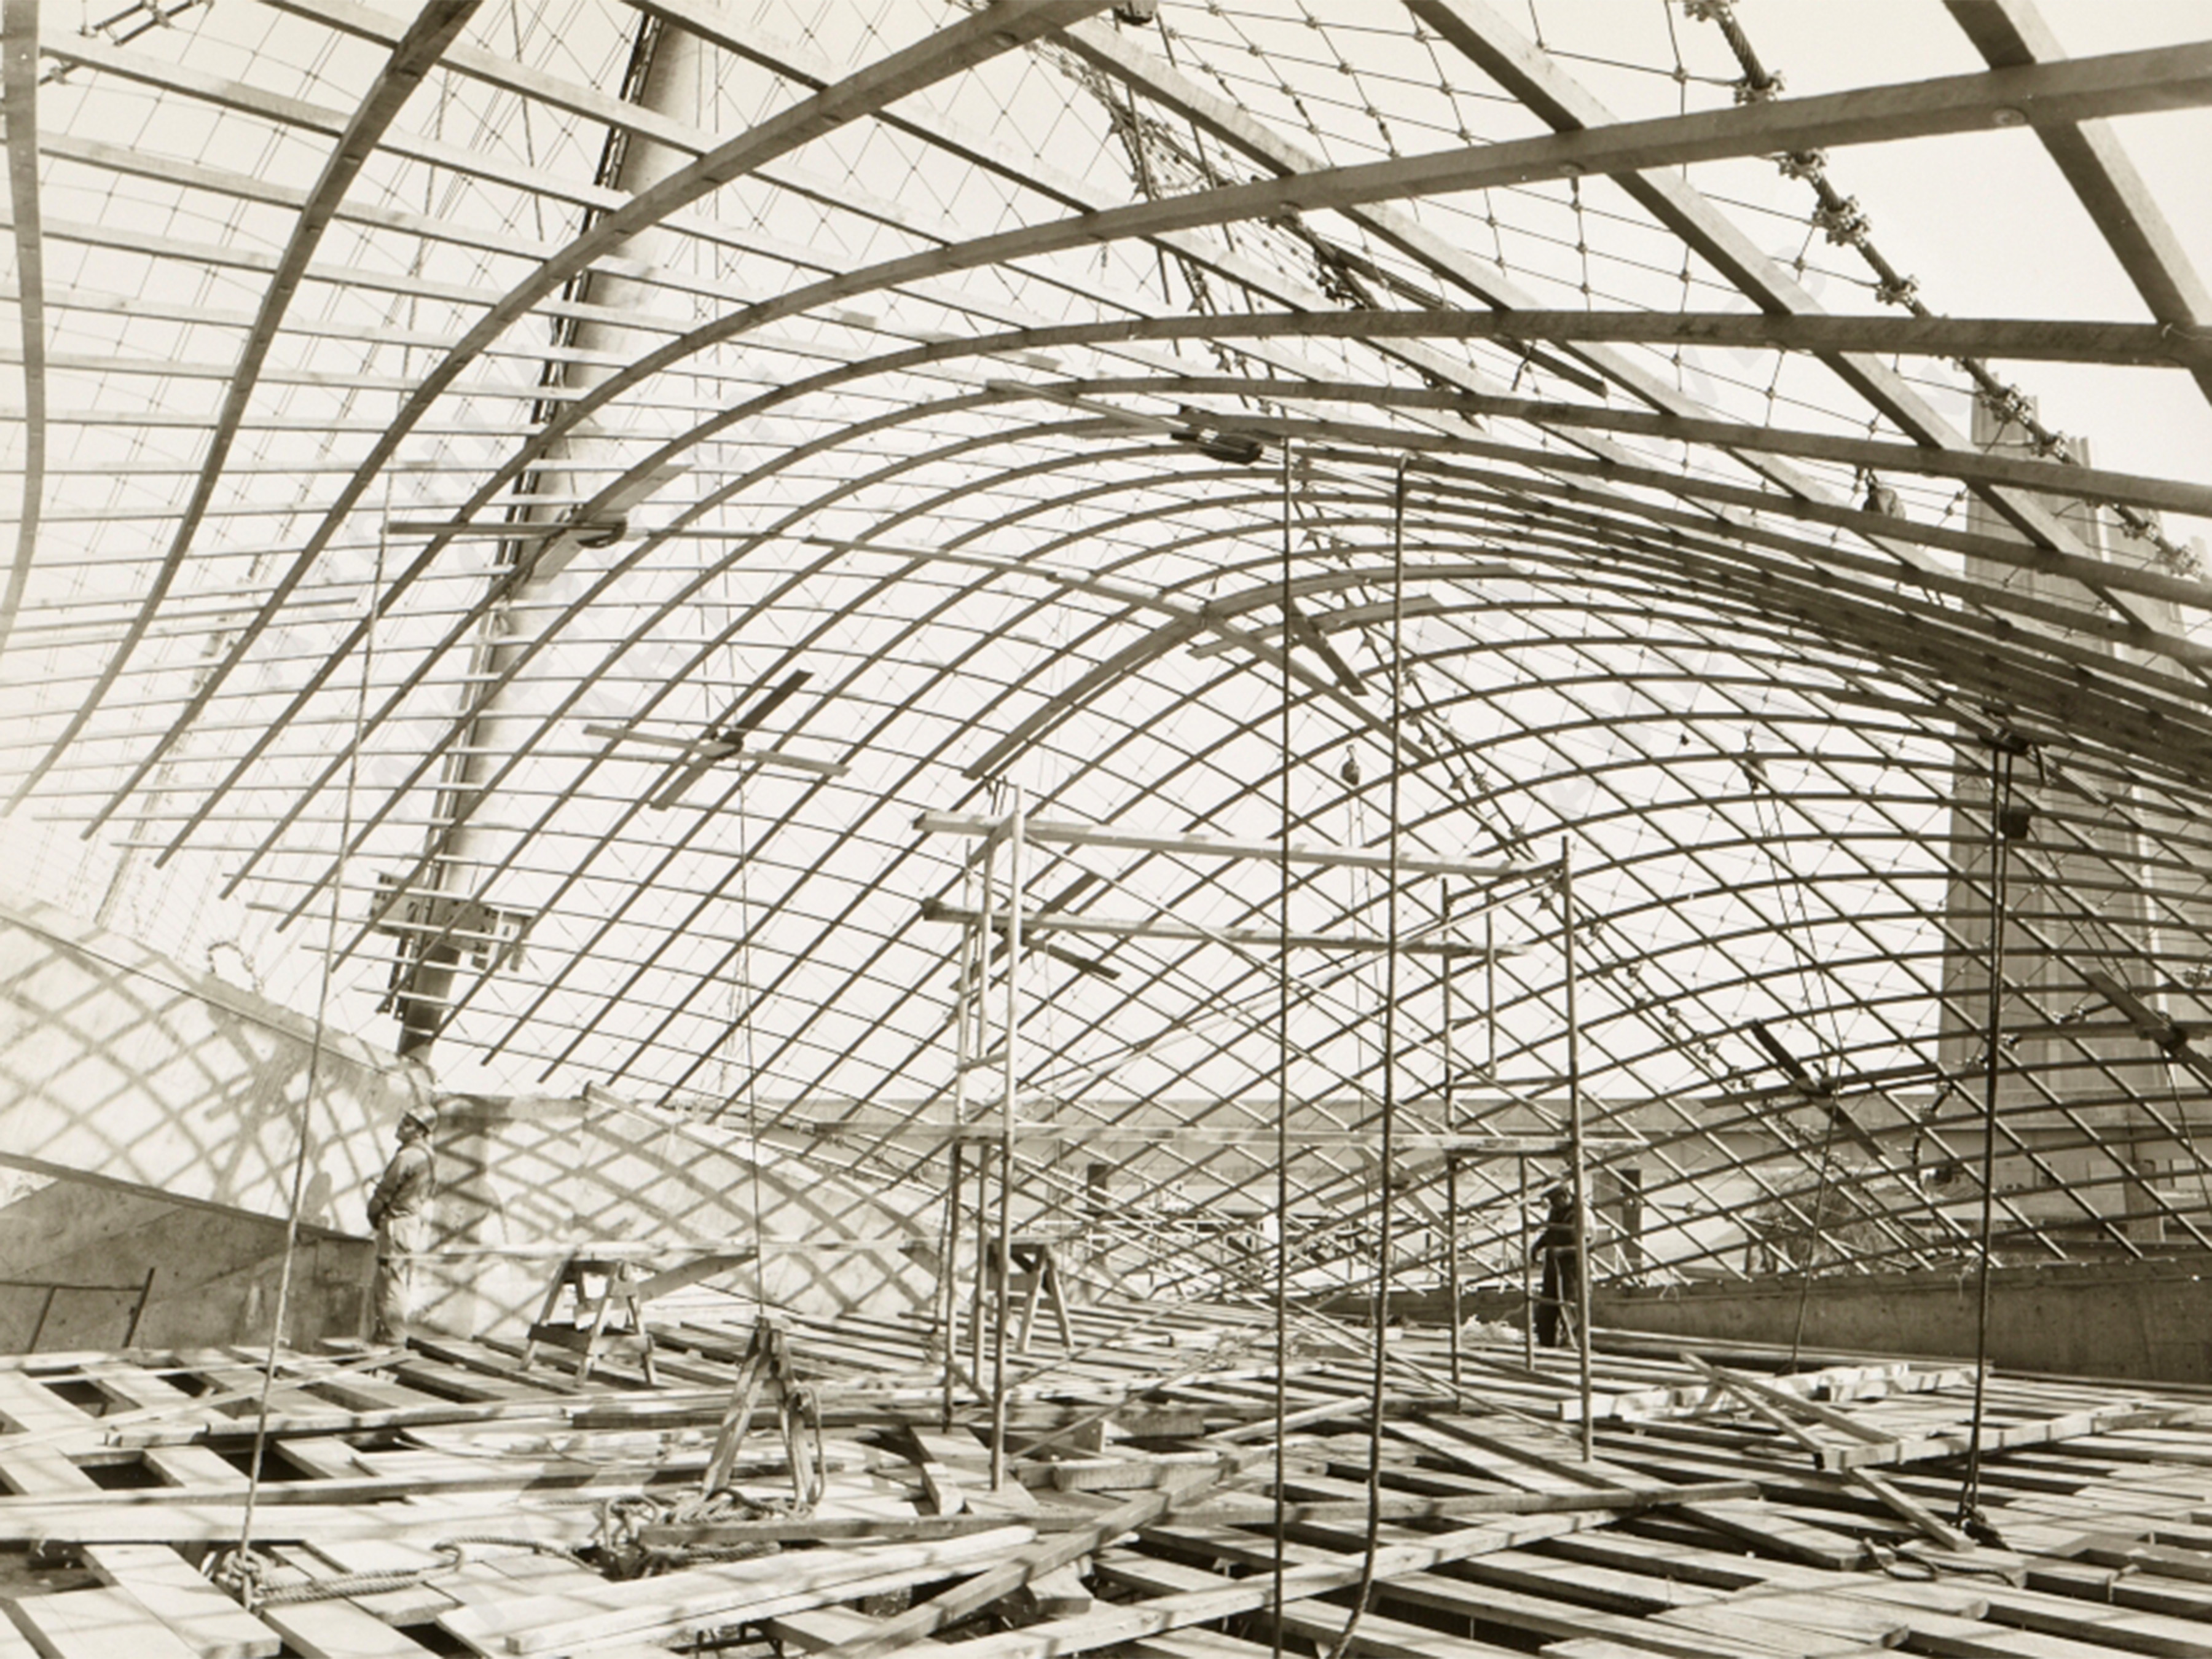
\includegraphics[width=0.48\textwidth]{montreal_lift.jpg}\label{fig:montreal_a}}
		\hspace*{\fill}
		\subfloat[][Inside view]{\includegraphics[width=0.48\textwidth]{montreal_inside.jpg}\label{fig:montreal_b}}
		%
		\vspace{10pt}
		\caption{Timber gridshell built in 1967 in Montreal, Canada.}
		\label{fig:montreal}    
\end{figure}
It is worth to mention that several unexecuted large-scale projects were studied by Frei Otto between 1967 and 1973 at the \emph{IL} or at the \emph{Atelier Warmbronn}.\footnote{Atelier Warmbronn is the architectural studio founded by Frei Otto in 1969.} These projects are basically documented in \cite[pp.~278 - 288]{IL10} and reveal that he was training his capacity to master large-scale projects with the technic of elastic gridshells for more conventional building projects (wave pool, swimming hall, multi-purpose hall, auditorium, \telp{}).

\subsubsection{The Mannheim Multihalle : the completion of a decade of research}
The project of the Multihalle started in 1970, when the decision was made that Mannheim, Germany, would hold the Bundesgartenschau in 1975.\footnote{The Bundesgartenschau is a national horticultural exibithion that takes place every two years in Germany.} The architects of the project, \emph{Carl Mutschler \& Partners}, consulted Frei Otto at \emph{Atelier Warmbronn} as he was starting to get known in the filed of innovative lightweight structures. This is how the idea of the gridshell was introduced in the project \cite{Liddell2015}. 

A thorough report on the project is available in \cite{IL13}.  A more condensed but still precise description of the engineering problematics related to this projects are availlables in the excellent papers from \citet{Happold1975, Liddell2015}.

Mannheim is an unprecedented realization because it is more than twenty times larger than the previously built gridshells in Montreal and is meant to last many years and not only for the duration of a short-term exhibition. The timber lattice, still existing in 2017,  covers an area of \SI{7400}{m^2}. It is composed of two interconnected domes, one for the multi-purpose hall (span : \SI{60}{m} | height : \SI{20}{m}) and one for the restaurant (span : \SI{50}{m} | height : \SI{18}{m}).
\begin{figure}[H]
		\subfloat[][Inside view]{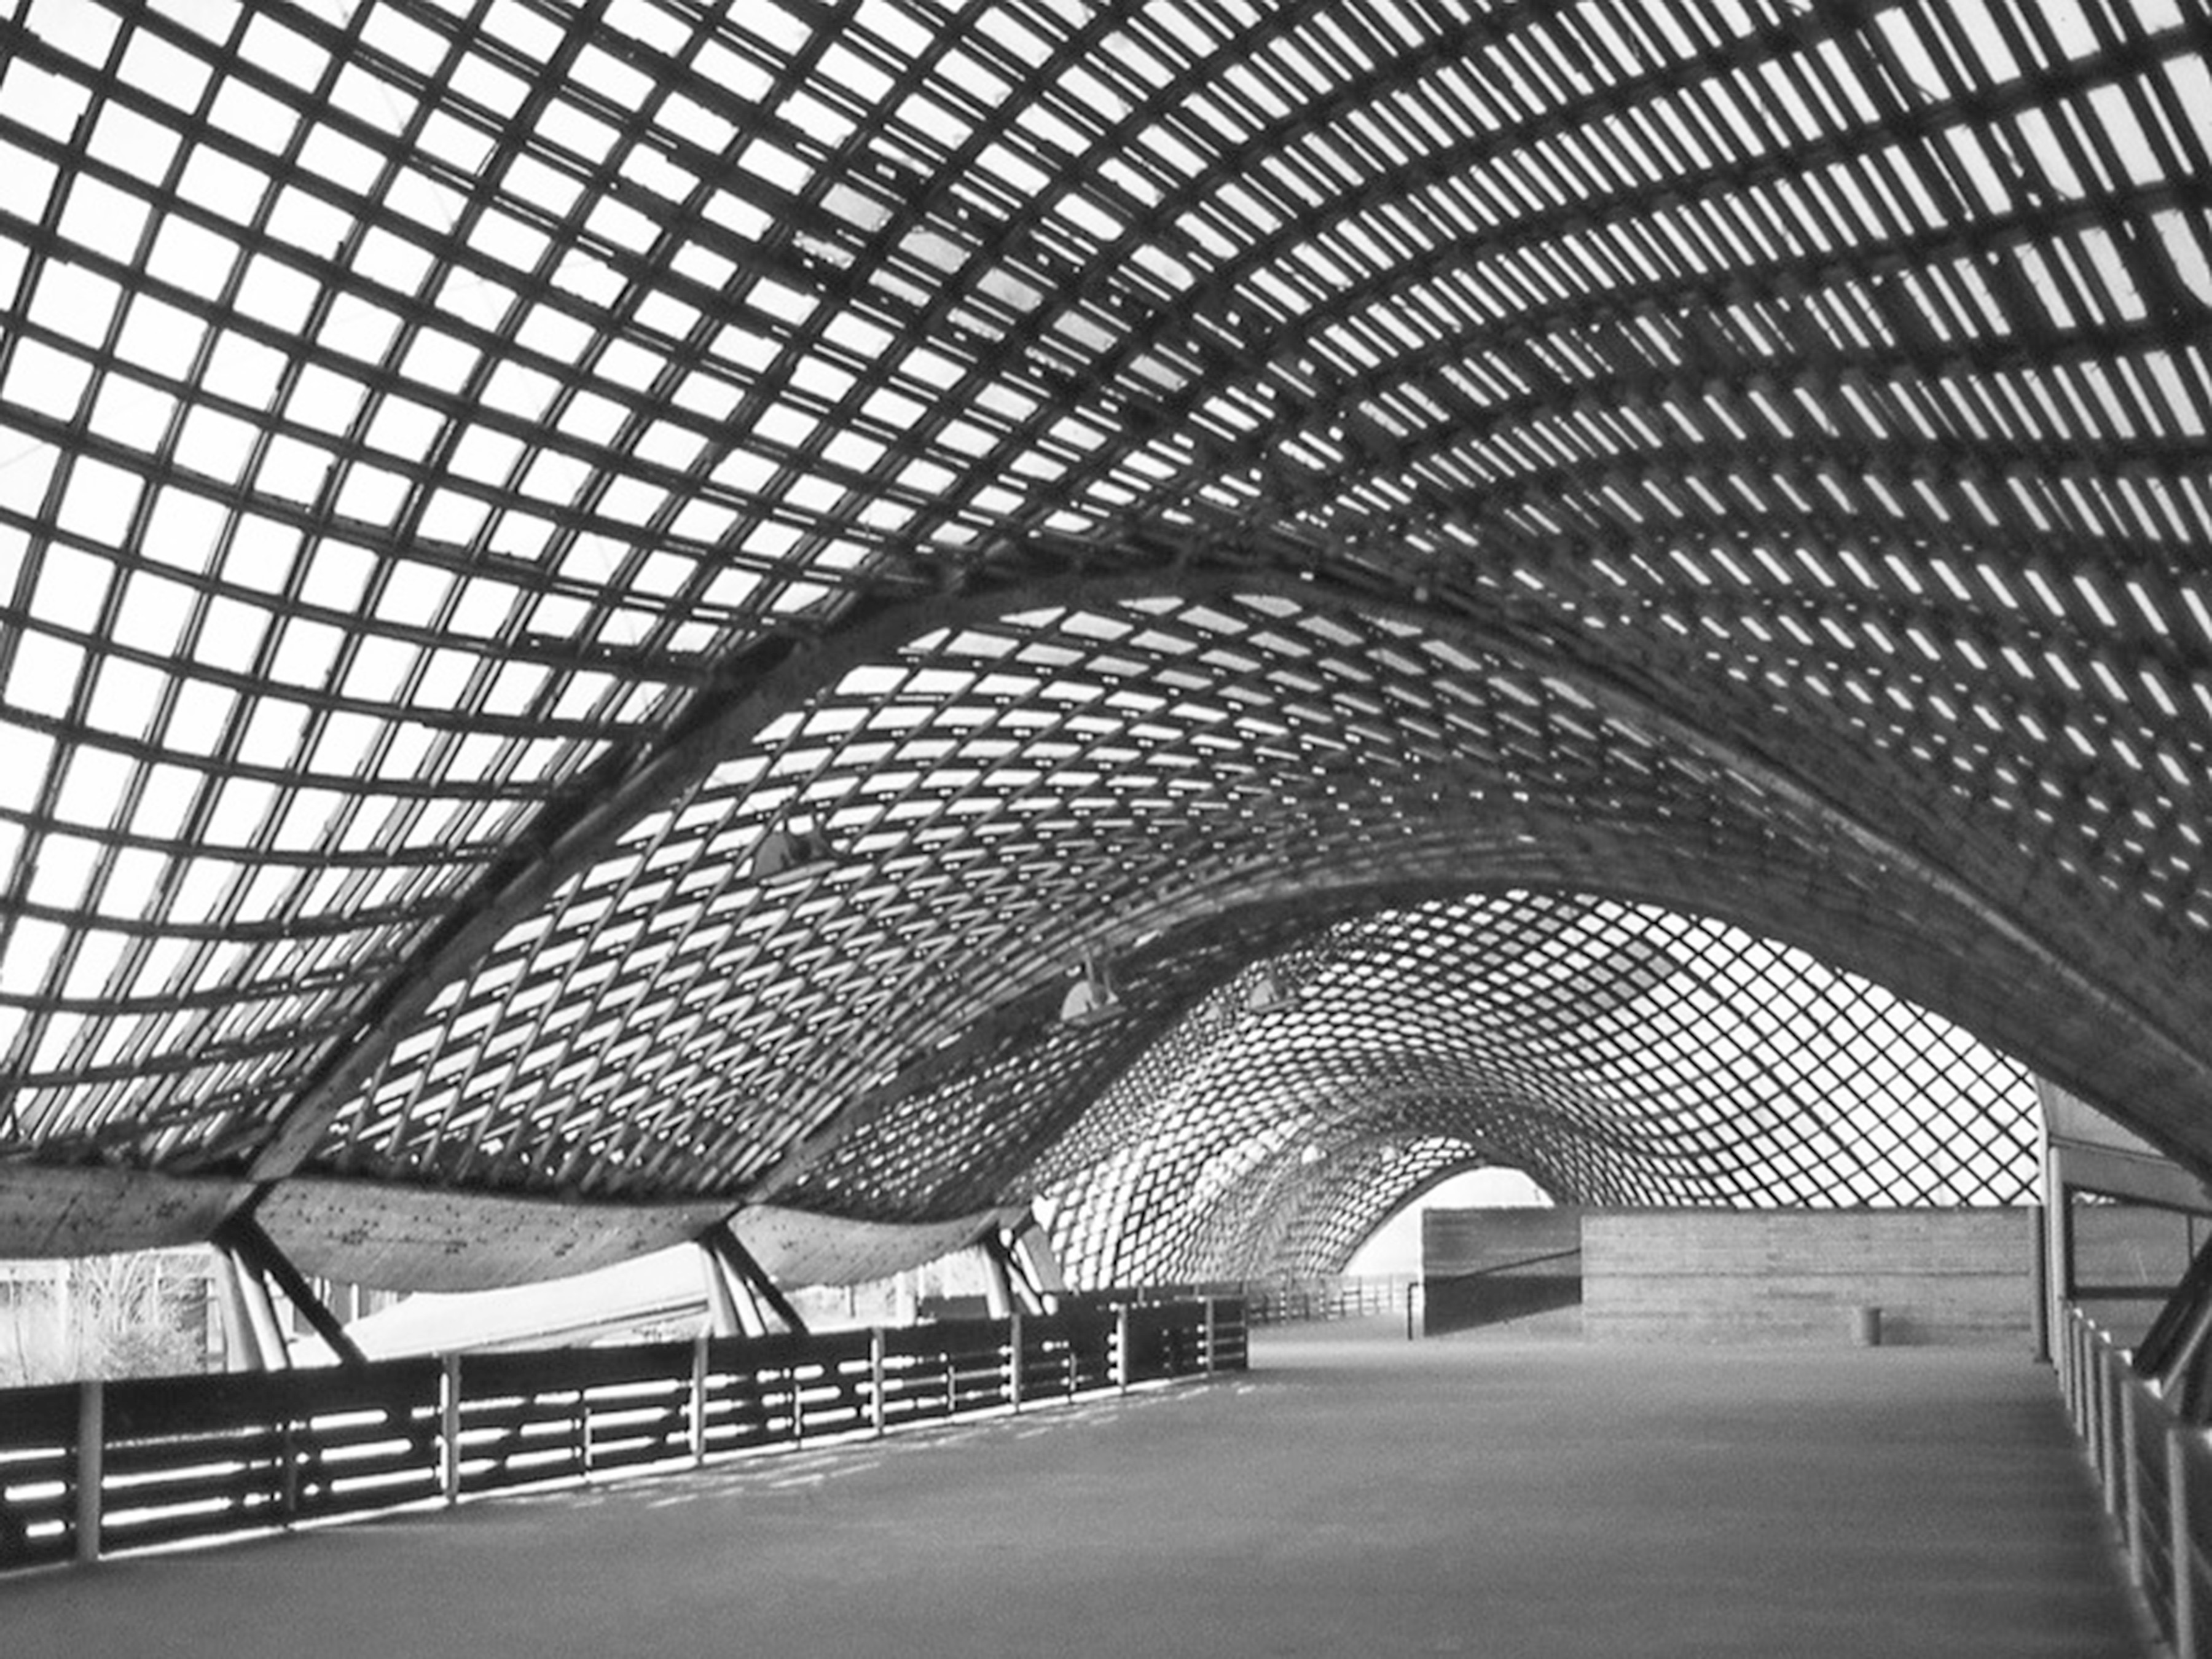
\includegraphics[width=0.48\textwidth]{mannheim_inside.jpg}\label{fig:montreal_a}}
		\hspace*{\fill}
		\subfloat[][Sky view]{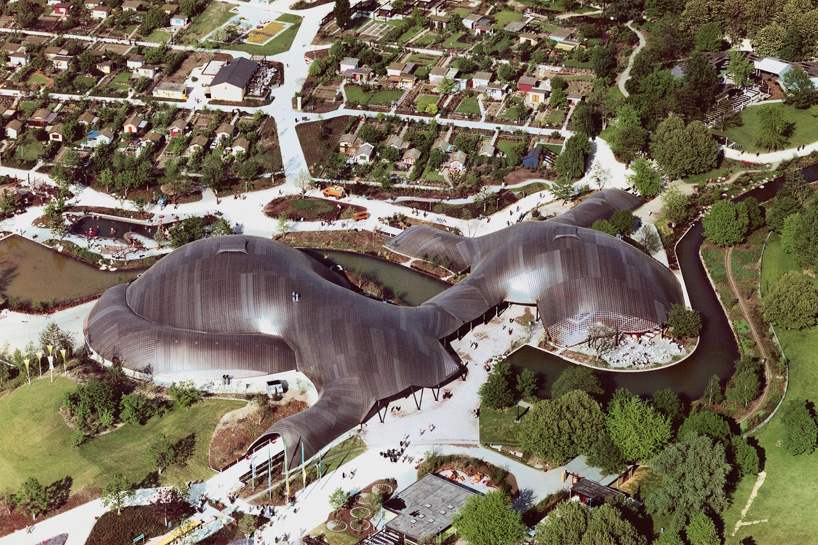
\includegraphics[width=0.48\textwidth]{mannheim_sky.jpg}\label{fig:montreal_b}}
		%
		\vspace{10pt}
		\caption{Timber gridshell built in 1975 in Mannheim, Germany.}
		\label{fig:mannheim}    
\end{figure}

Although the constructif system deployed at Mannheim clearly inherited from the previous developments, the challenge was such that it had to be revisited. In particular the main additions were the introduction of the double layer system and the proper bracing of the grid. A major advance was also the use of the very first numeric models to study the structure. 

The double layer system was introduced to tackle a two issues~: the grid needed some flexibility to be bent into the desired shape, but once erected it should provide sufficient bending stiffness to resist disturbing loads and avoid a buckling collapse.\footnote{Theoretically, self-weight loads would produce only compression in the members because the (funicular) form of the grid resulted from the inversion of a hanging chain model in pure tension.} One erected, the two grids, one sliding on top of the other one, were connected together to form a single grid with much higher ladder profiles (from \SI{50}{mm} to \SI{150}{mm}), increasing their bending stiffness by 26. 

Because the in-plane stiffness of the grid also plays a major role in the resistance to buckling, this question was considered with care. The bracing of the grid was first achieved by preventing the nodes to turn once the grid was erected. This was done by creating some friction in the nodes when tightening the bolts linking the laths, after the grid was erected. Additional bracing cables were put in the grid.

Finally, the project of Mannheim was a key project in the development of modern lightweight structures. Great engineers were born in touch with Frei Otto, following its footsteps or collaborating with him. This heritage has irrigated for several decades the engineering of lightweight structures in Europe and gave birth, directly or indirectly, to several studios among which we can cite \emph{Buro Happold}, \emph{Schlaich Bergermann \& Partner} and \emph{RFR}.

\subsubsection{The dry period : 25 years from Mannheim to Hannover}

Although the experience of Mannheim proved the feasibility and the potential of gridshell structures for large-scale projects, it also revealed that these projects were subject to an incredible complexity in terms of structural design, geometry, modeling, testing, team work, construction methods, \telp{} At that time, only few people could pretend to master all the knowledge and technics required to design and built timber gridshells and developed in the bosom of the \emph{Institute for Lightweight Structures} in Stuttgart. 

This project was obviously well ahead of its time and the engineering cost to design such structures was probably prohibitive considering the tools available at that time. This certainly explains why no elastic gridshells were built during the 25 following years, despite the optimism of the pioneers of the Multihalle~: \blockcquote[]{Harris2003}{For many years after its completion, Happold promoted the benefit of the timber gridshell as a construction technique and stated that he could not understand why it had not been adopted more widely. He perceived the benefits to be in the efficiency of the construction method to enable doubly curved (shell) structures to be constructed quickly and cost effectively.}.

Note that around 1975 small workshop and experiments lead to the construction of several but small elastic gridshells, as reported in \cite{IL10}. \cref{fig:projectsbymaterial} presents a non-exhaustive but quite extensive list of known executed gridshell projects. The dry period is clearly visible.

\begin{figure}[p]
\begin{fullpage}
	\centering
	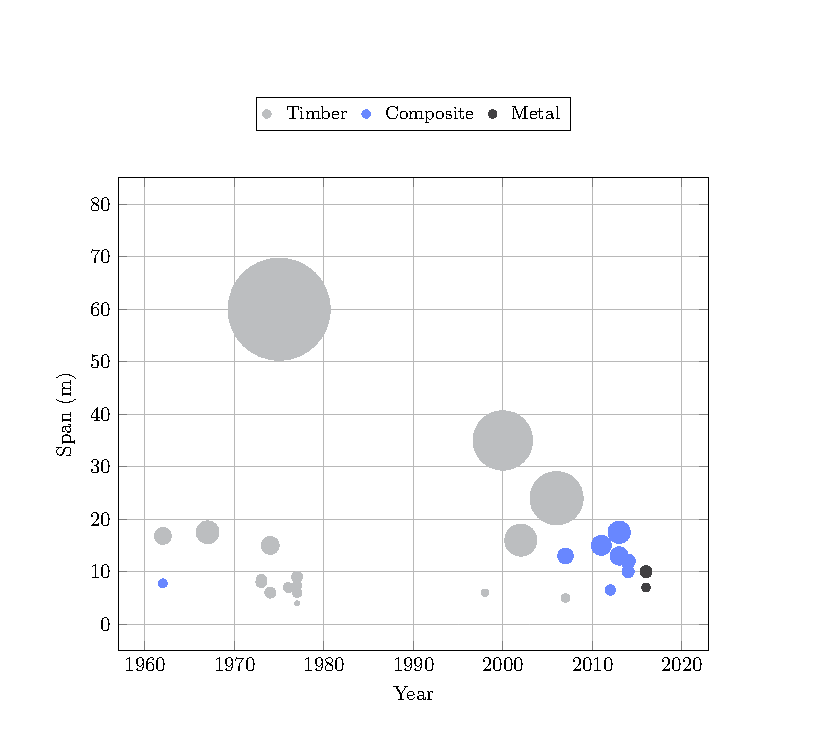
\includegraphics[]{ch1_gridshell/plot/1_projects/build.pdf}
	\caption[Known elastic gridshells built by the past.]{Known elastic gridshells built by the past. The surface of the bubbles is proportional to the covered area. Color indicates the material employed for the rods.}
	\label{fig:projectsbymaterial}
\end{fullpage}
\end{figure}

\subsubsection{The renewal : Hannover, Dowland and Savill}

\begin{figure}[H]
		\subfloat[][Interior view]{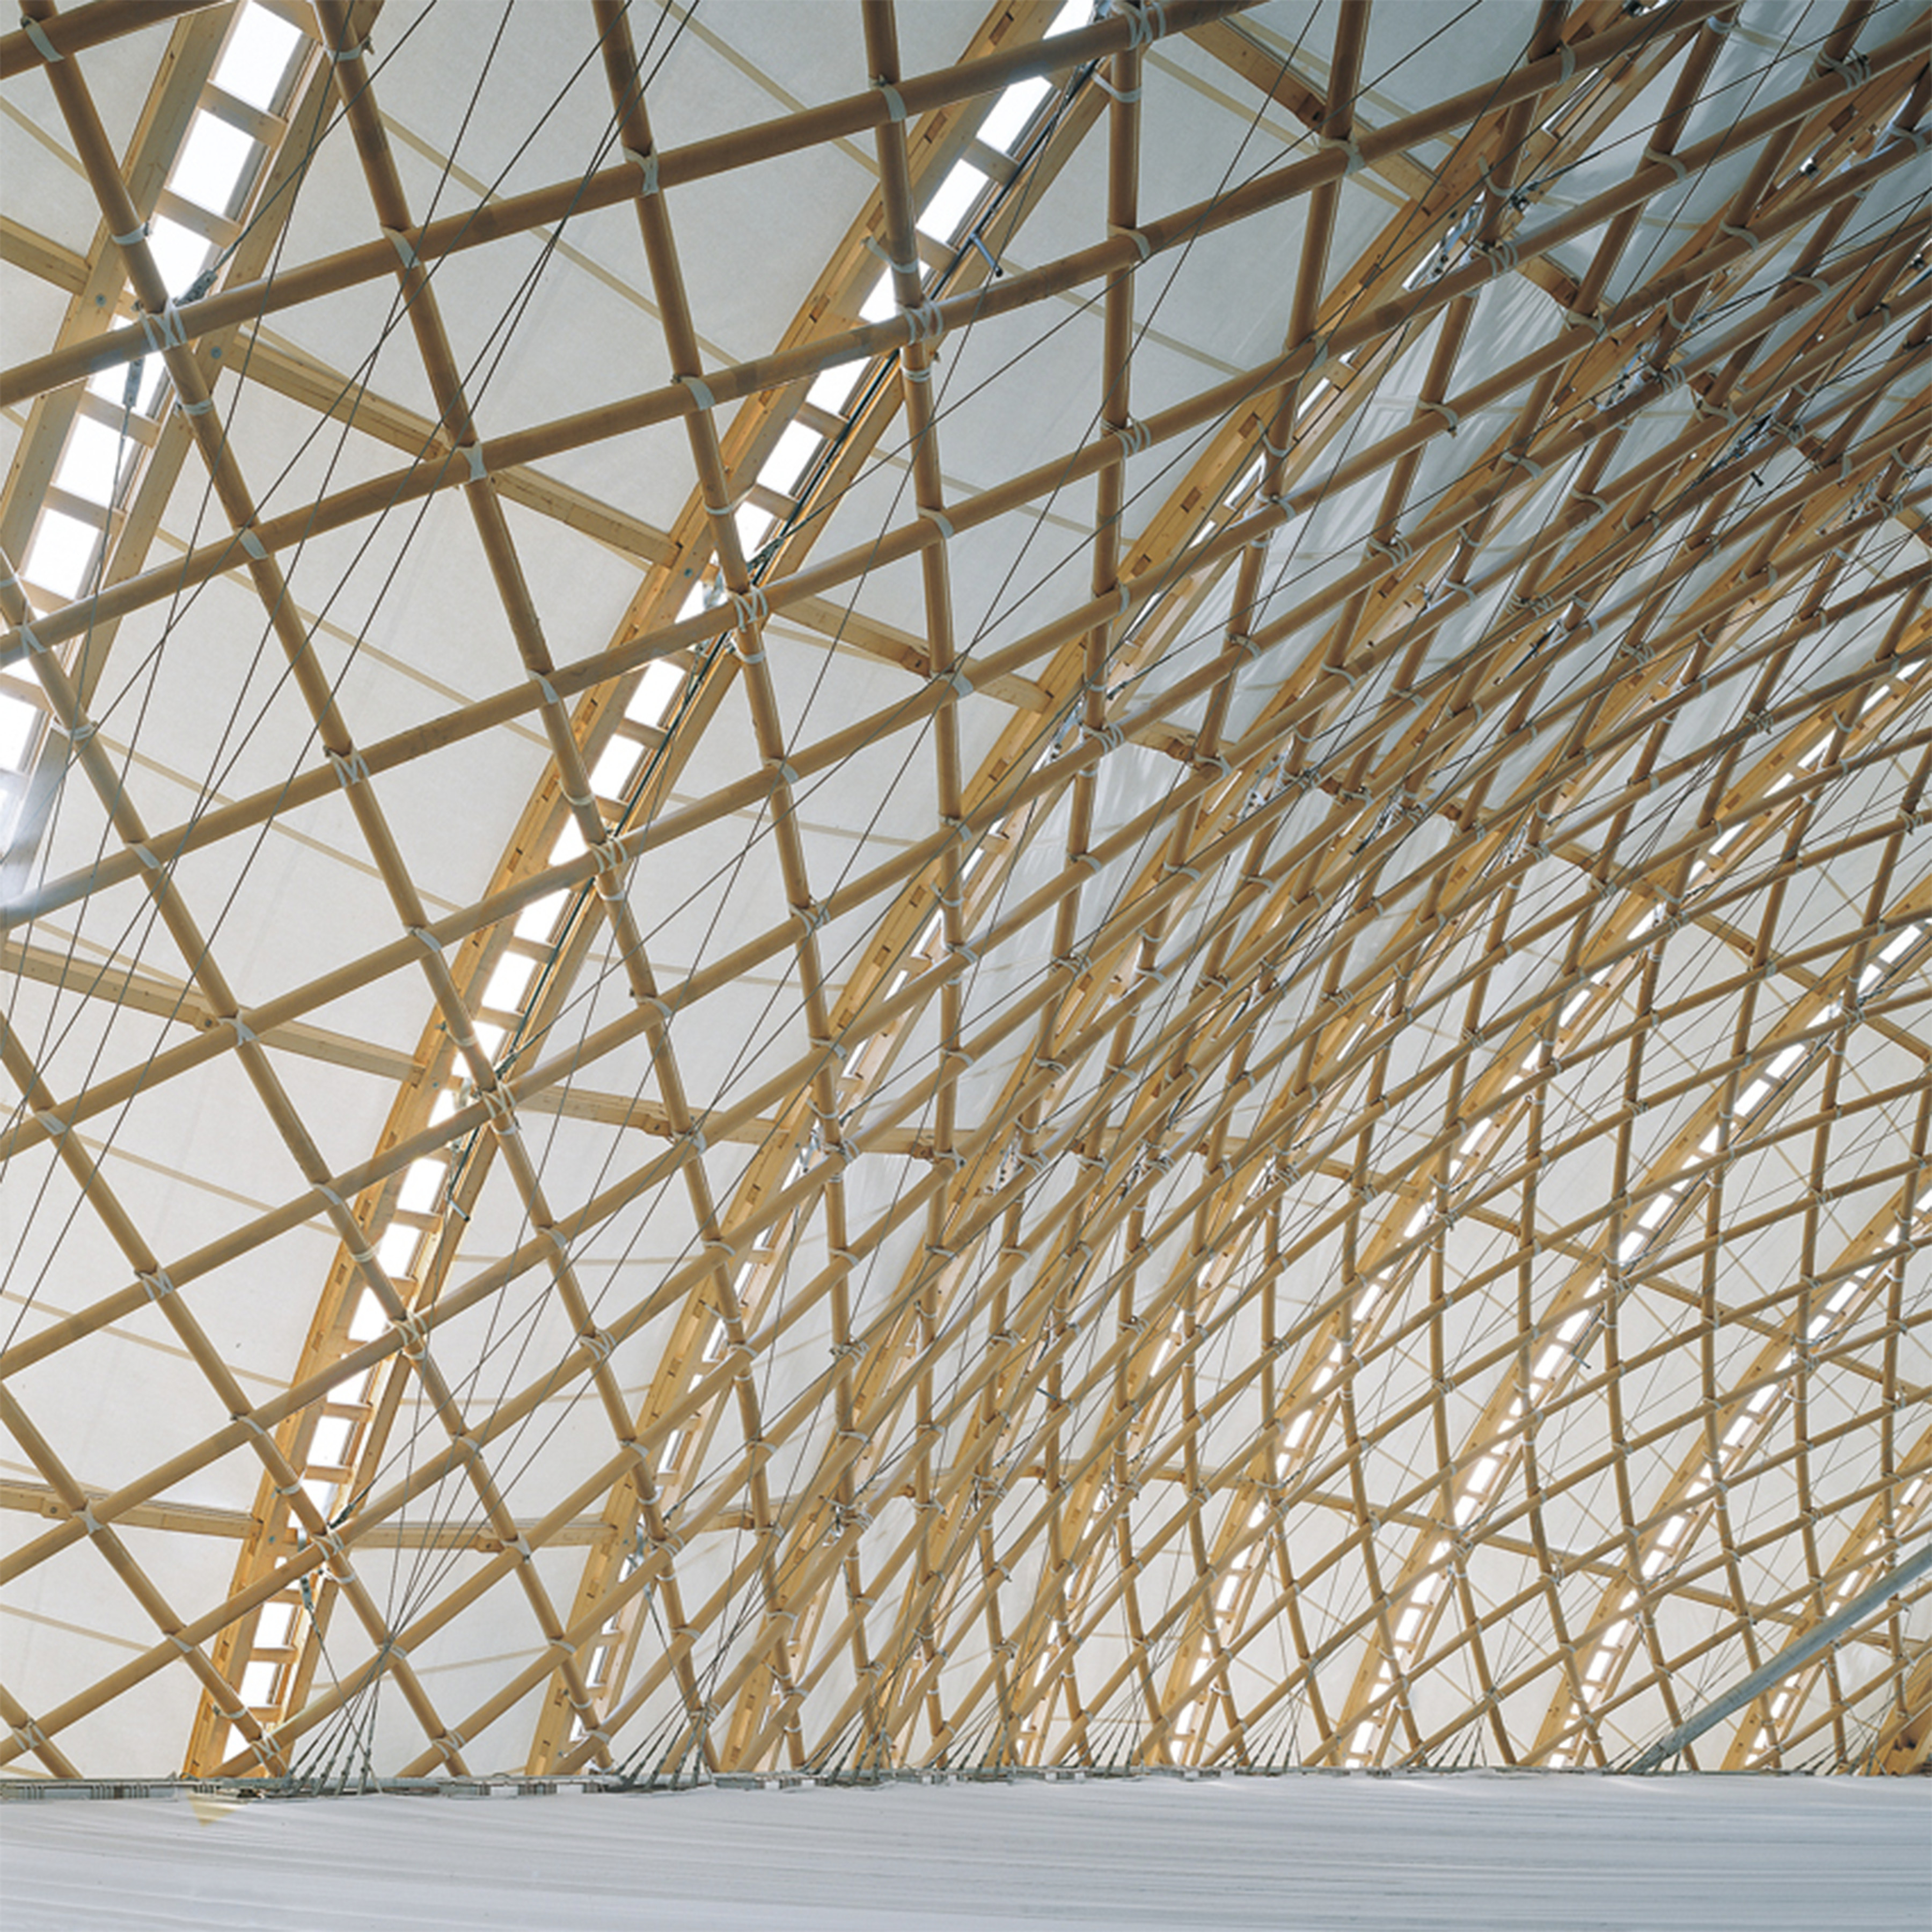
\includegraphics[width=0.32\textwidth]{tokyo_inside.jpg}\label{fig:tokyo_a}}
		\hspace*{\fill}
		\subfloat[][Sky view]{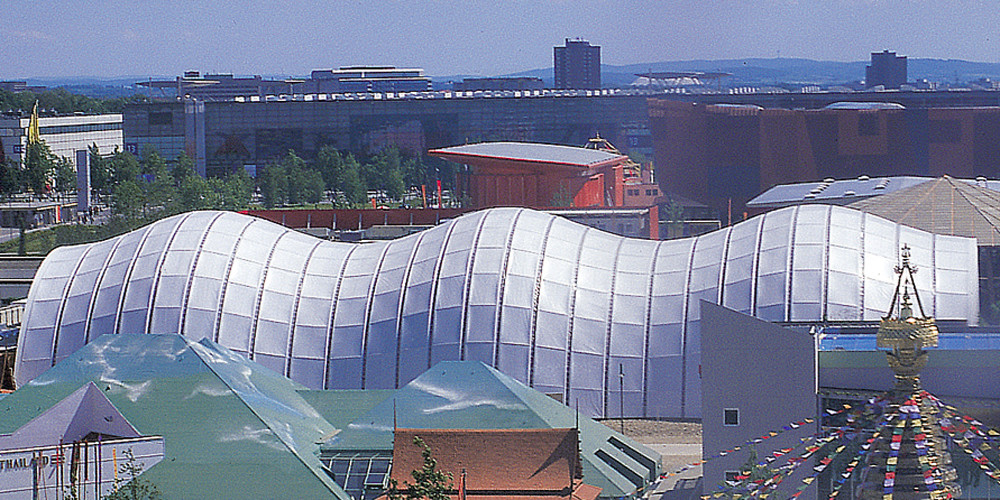
\includegraphics[width=0.64\textwidth]{tokyo_sky.jpg}\label{fig:tokyo_b}}
		%
		\vspace{10pt}
		\caption{Carboard gridshell built in 2000 in Hannover, Germany.}
		\label{fig:hannover}    
\end{figure}

 \begin{figure}[H]
		\subfloat[][Interior view]{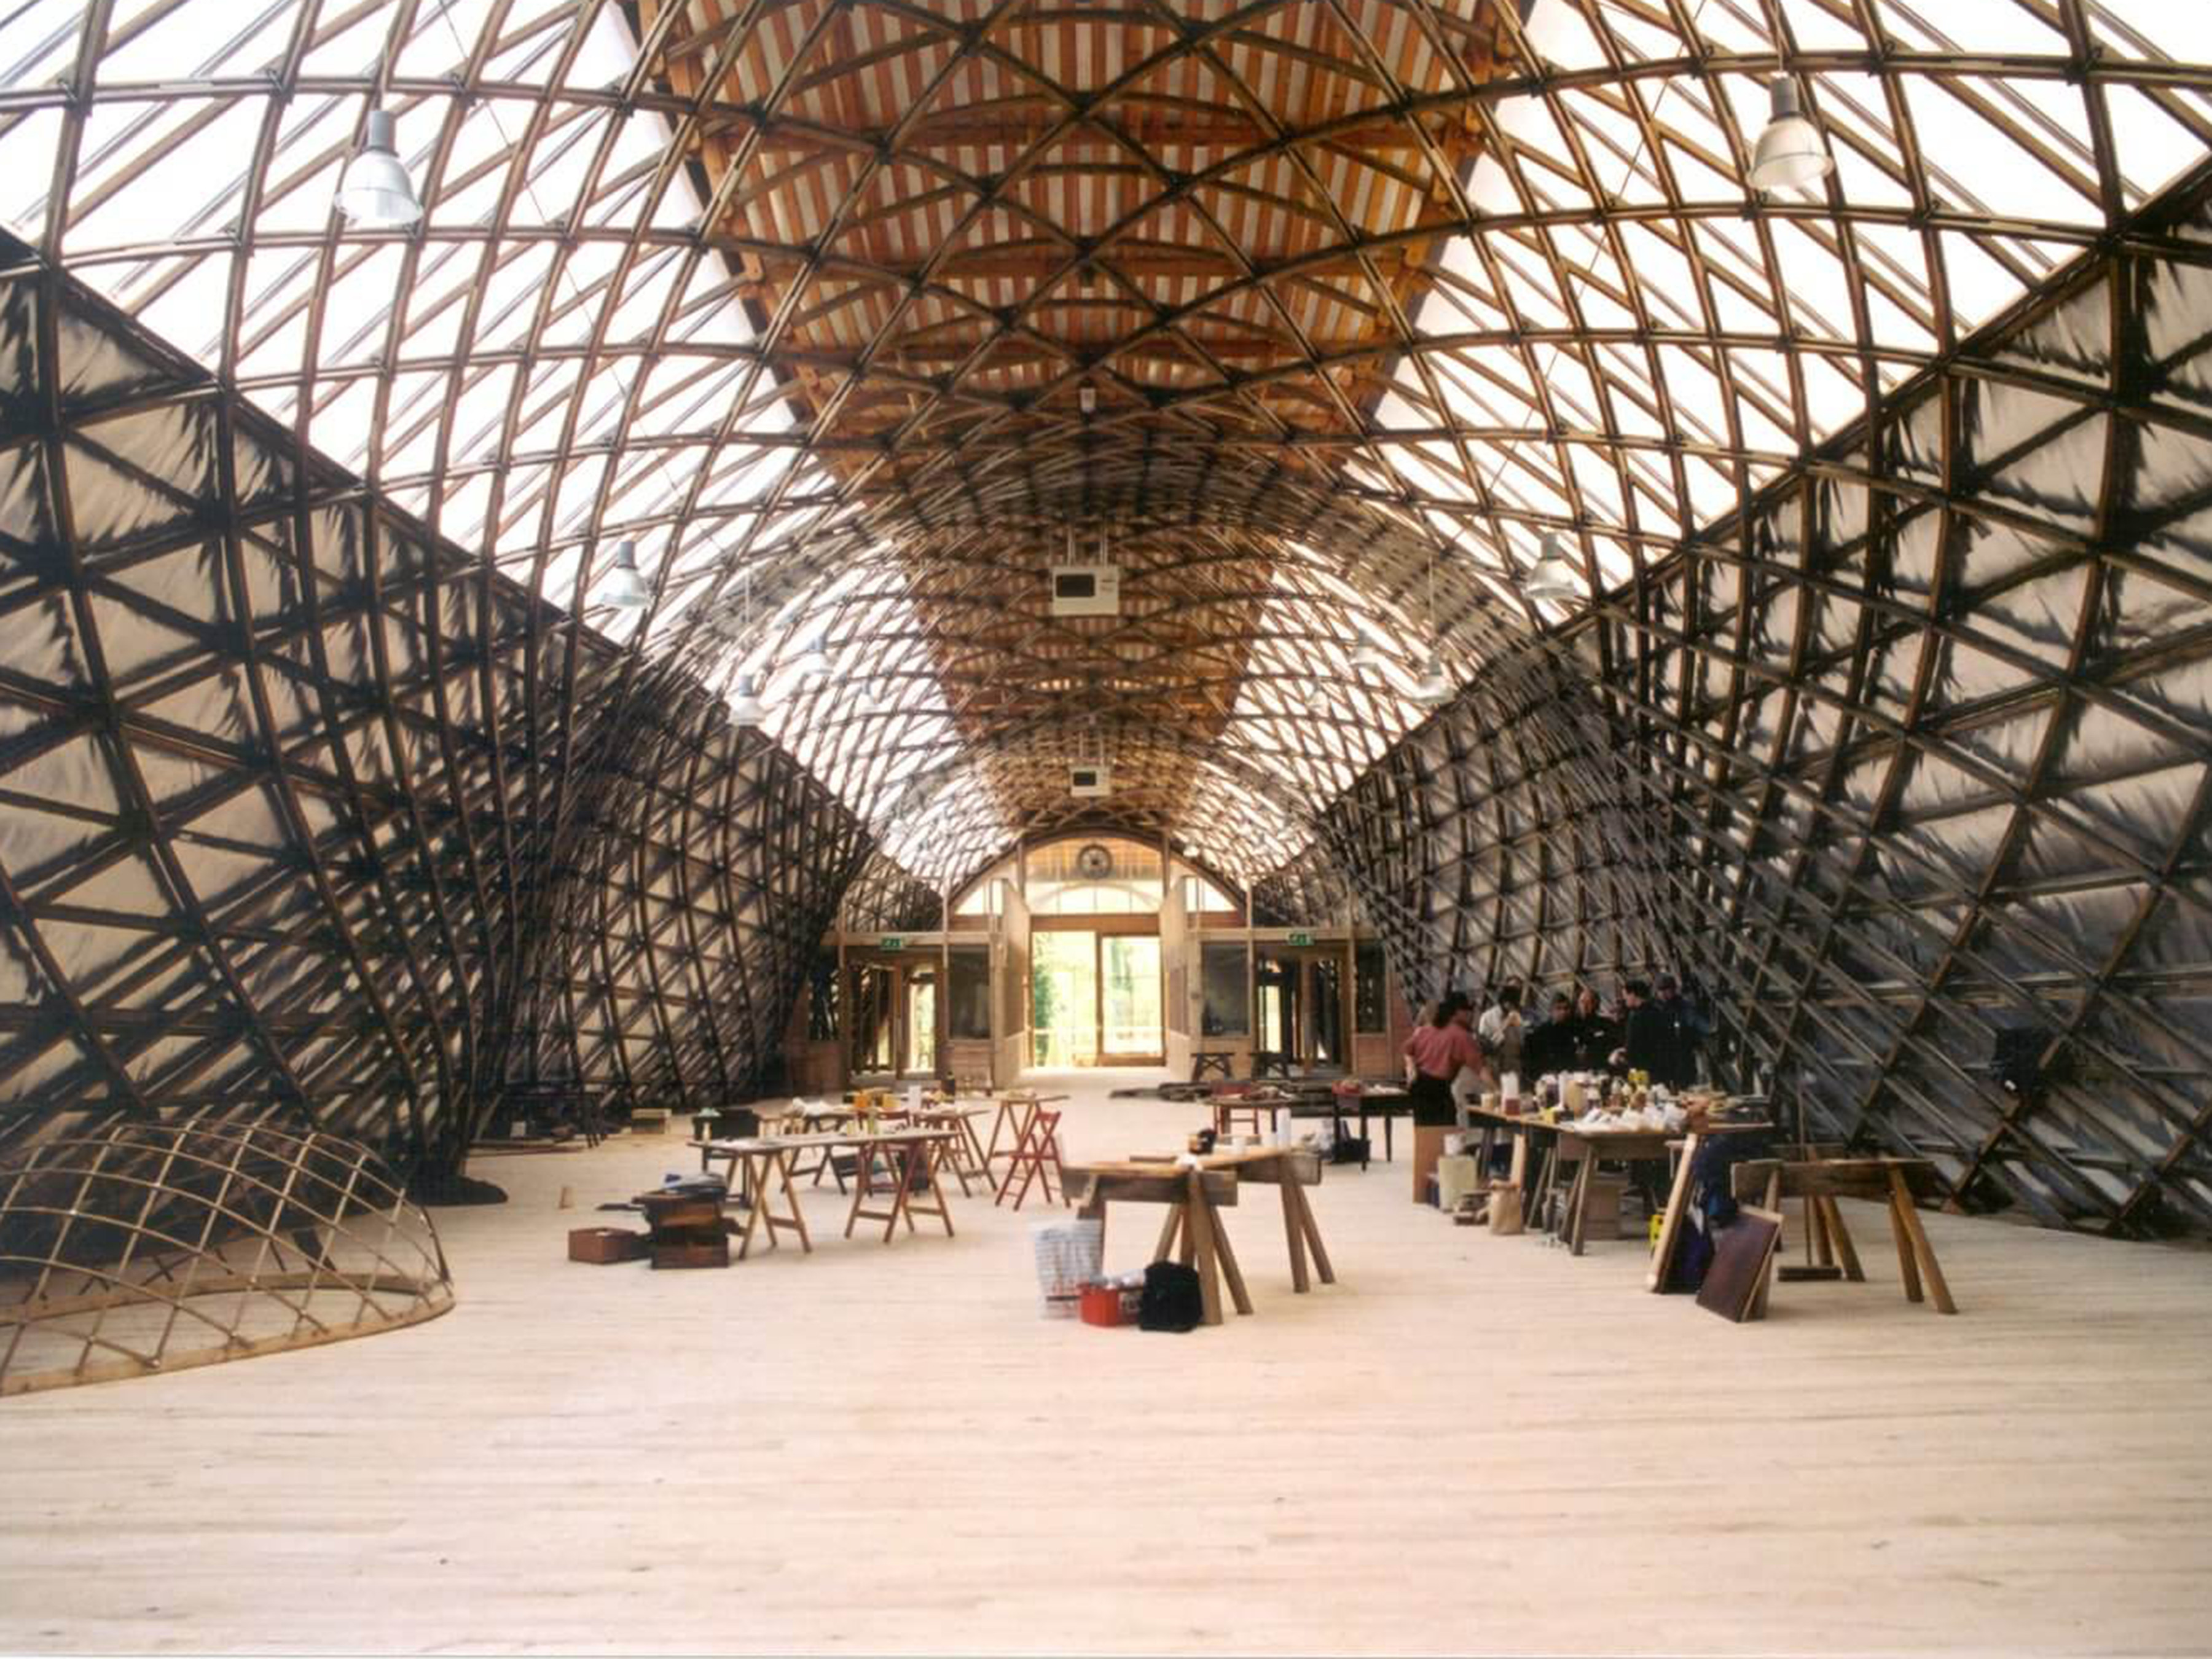
\includegraphics[width=0.48\textwidth]{downland_b.jpg}\label{fig:downland_a}}
		\hspace*{\fill}
		\subfloat[][Exterior view]{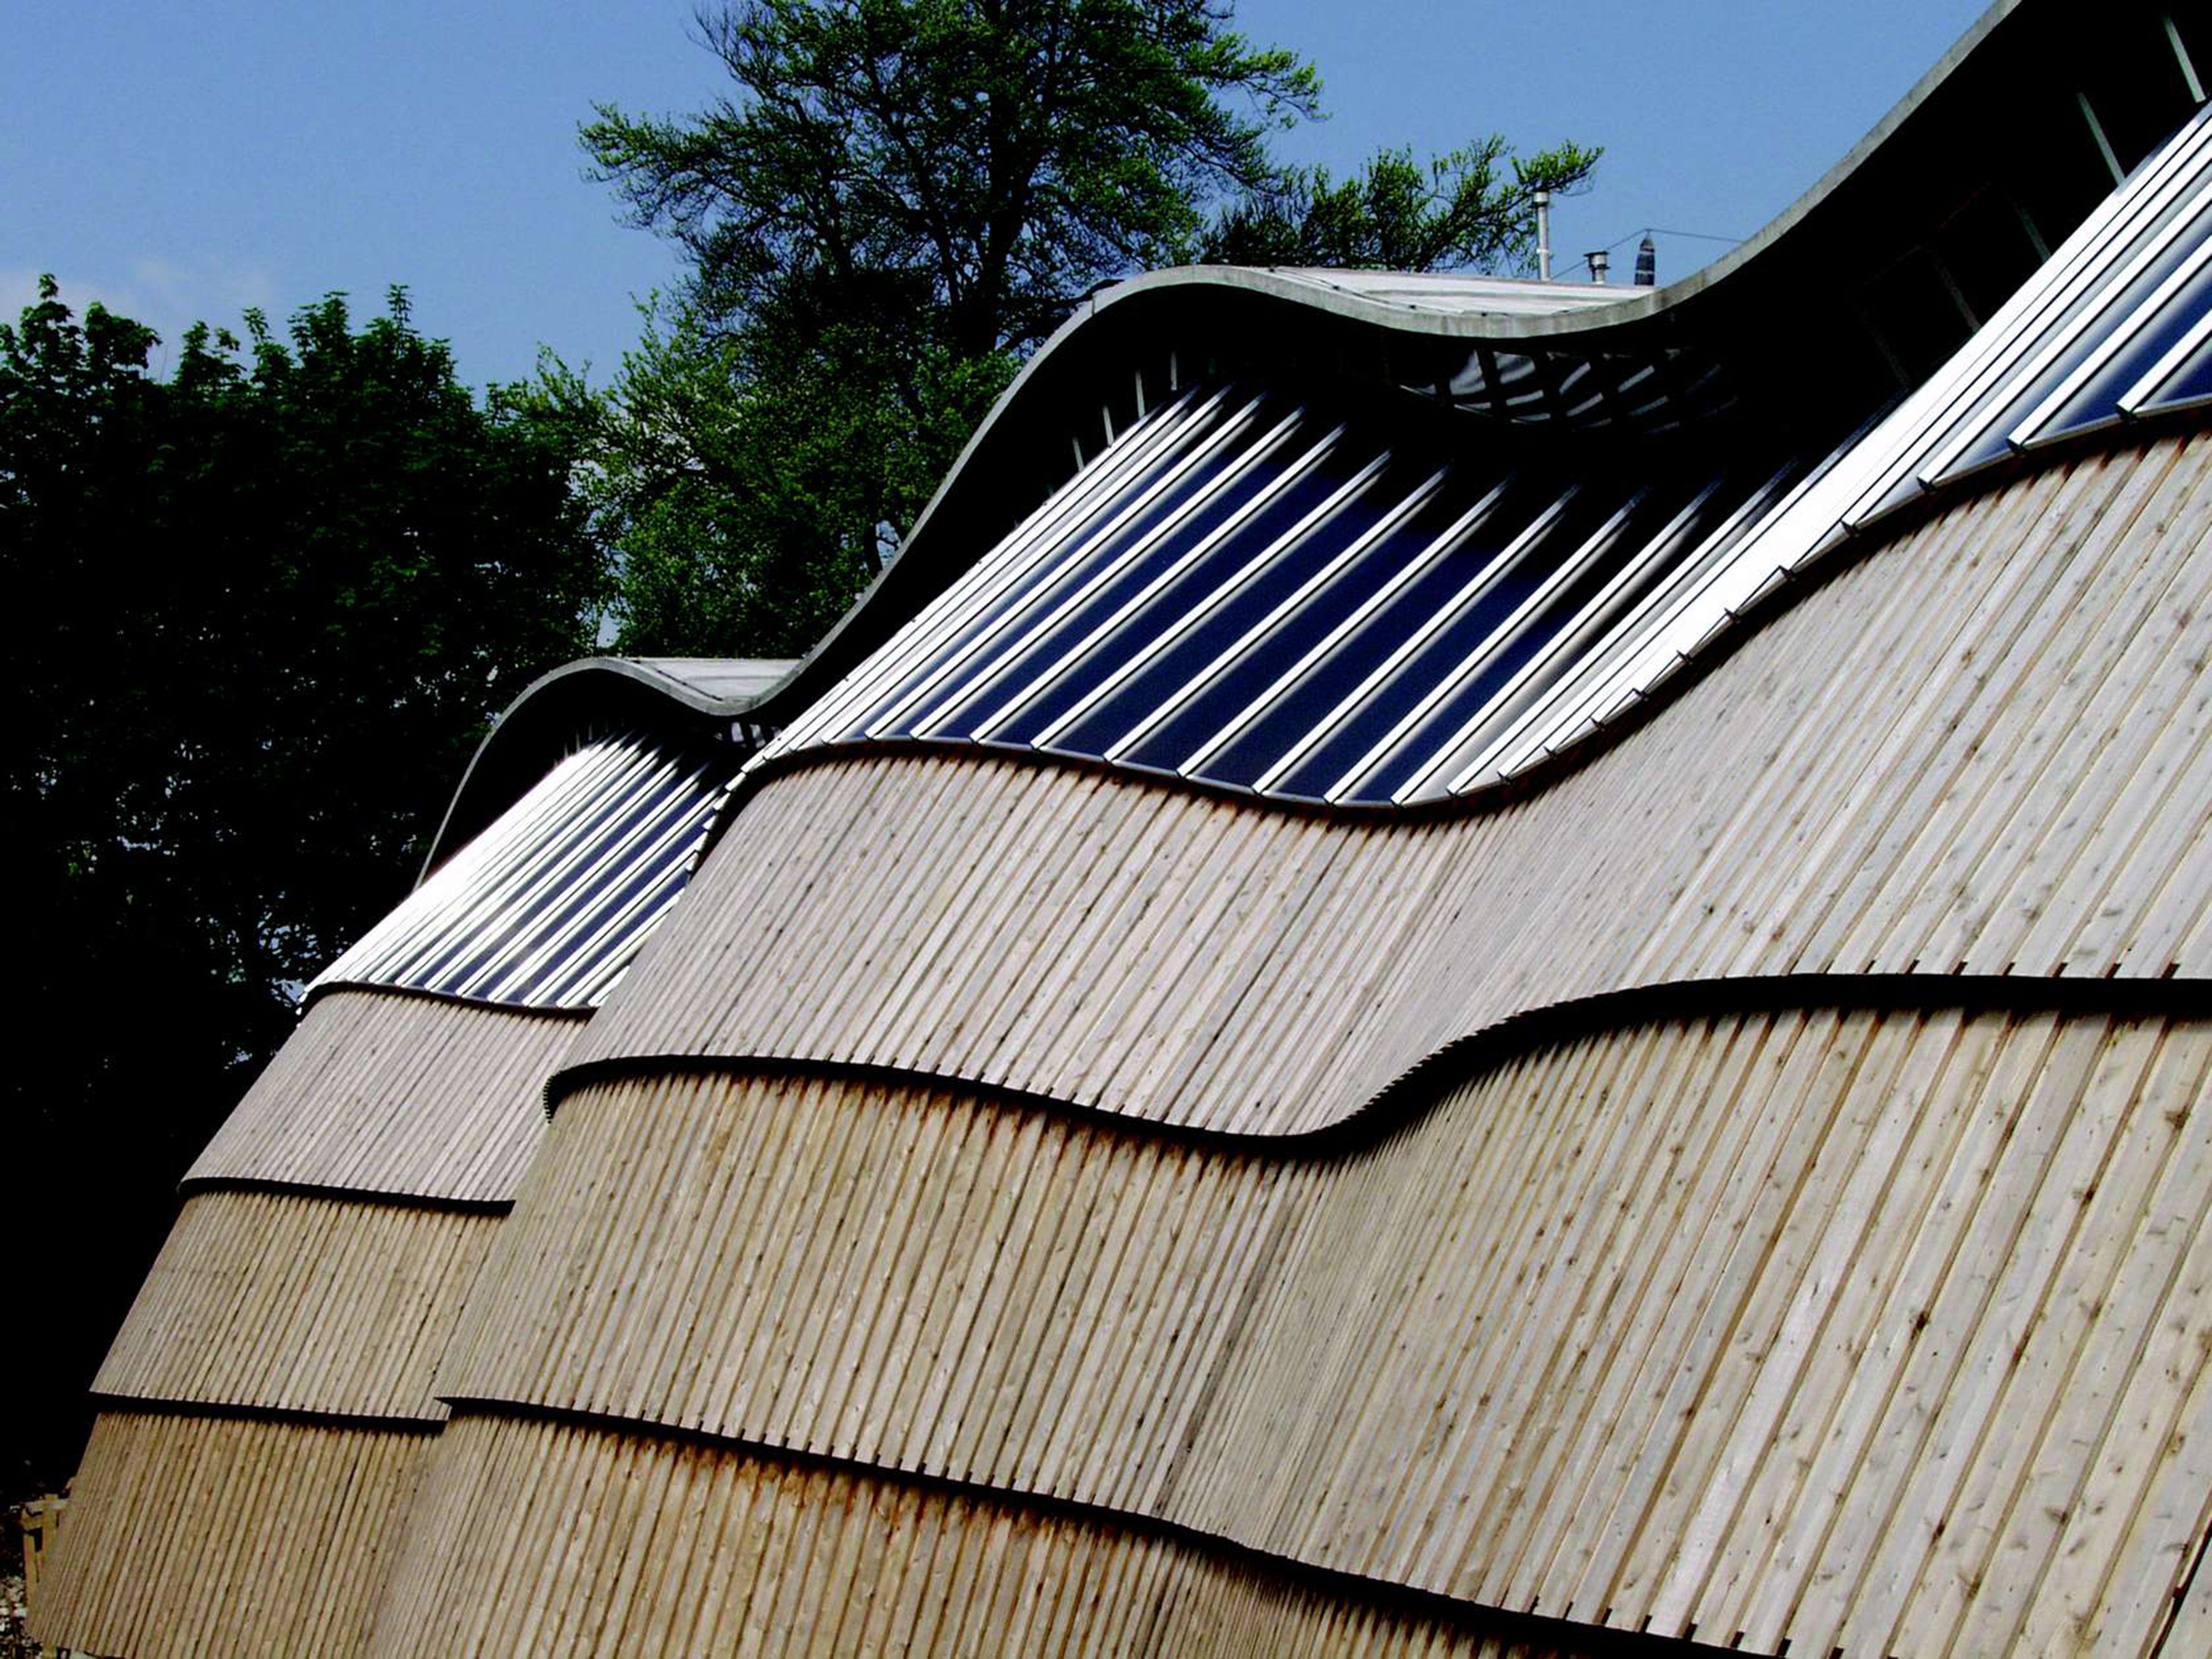
\includegraphics[width=0.48\textwidth]{downland_a.jpg}\label{fig:downland_b}}
		\vspace{10pt}
		\caption{Timber gridshell built in 2003 in Downland, England.}
		\label{fig:downland} 
\end{figure}

 \begin{figure}[H]
		\subfloat[][Interior view]{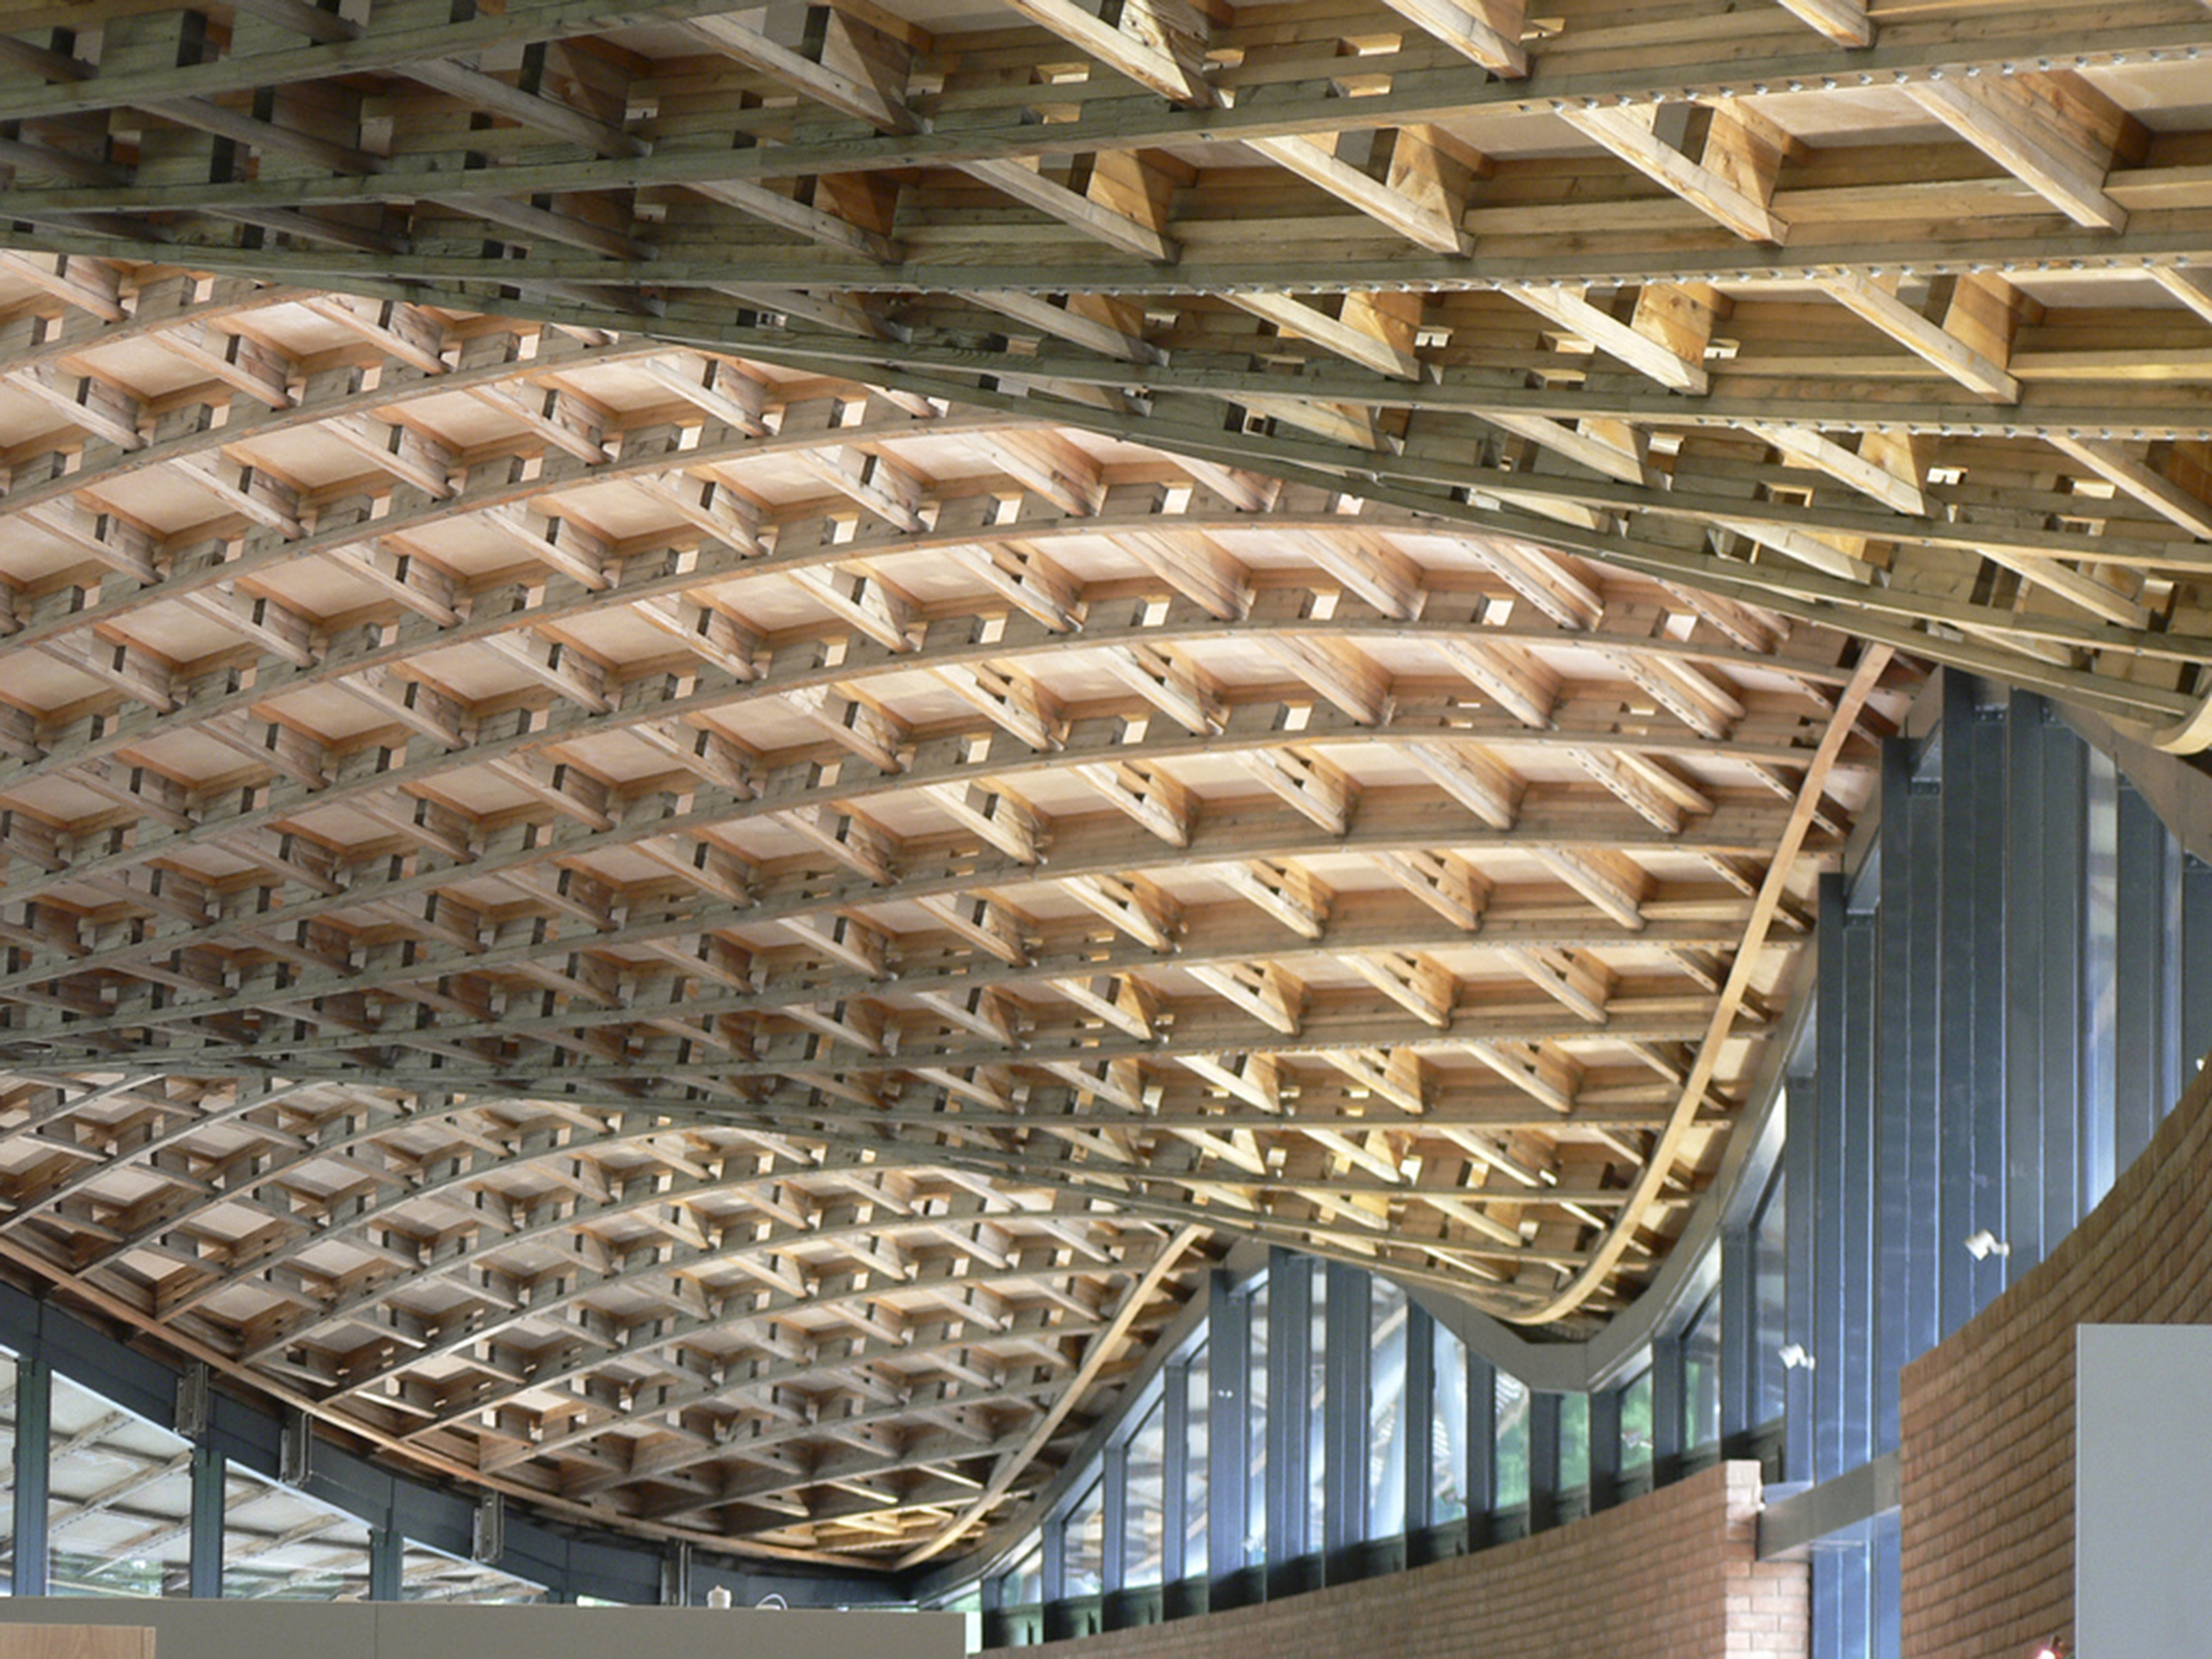
\includegraphics[width=0.48\textwidth]{savill_b.jpg}\label{fig:savill_a}}
		\hspace*{\fill}
		\subfloat[][Exterior view]{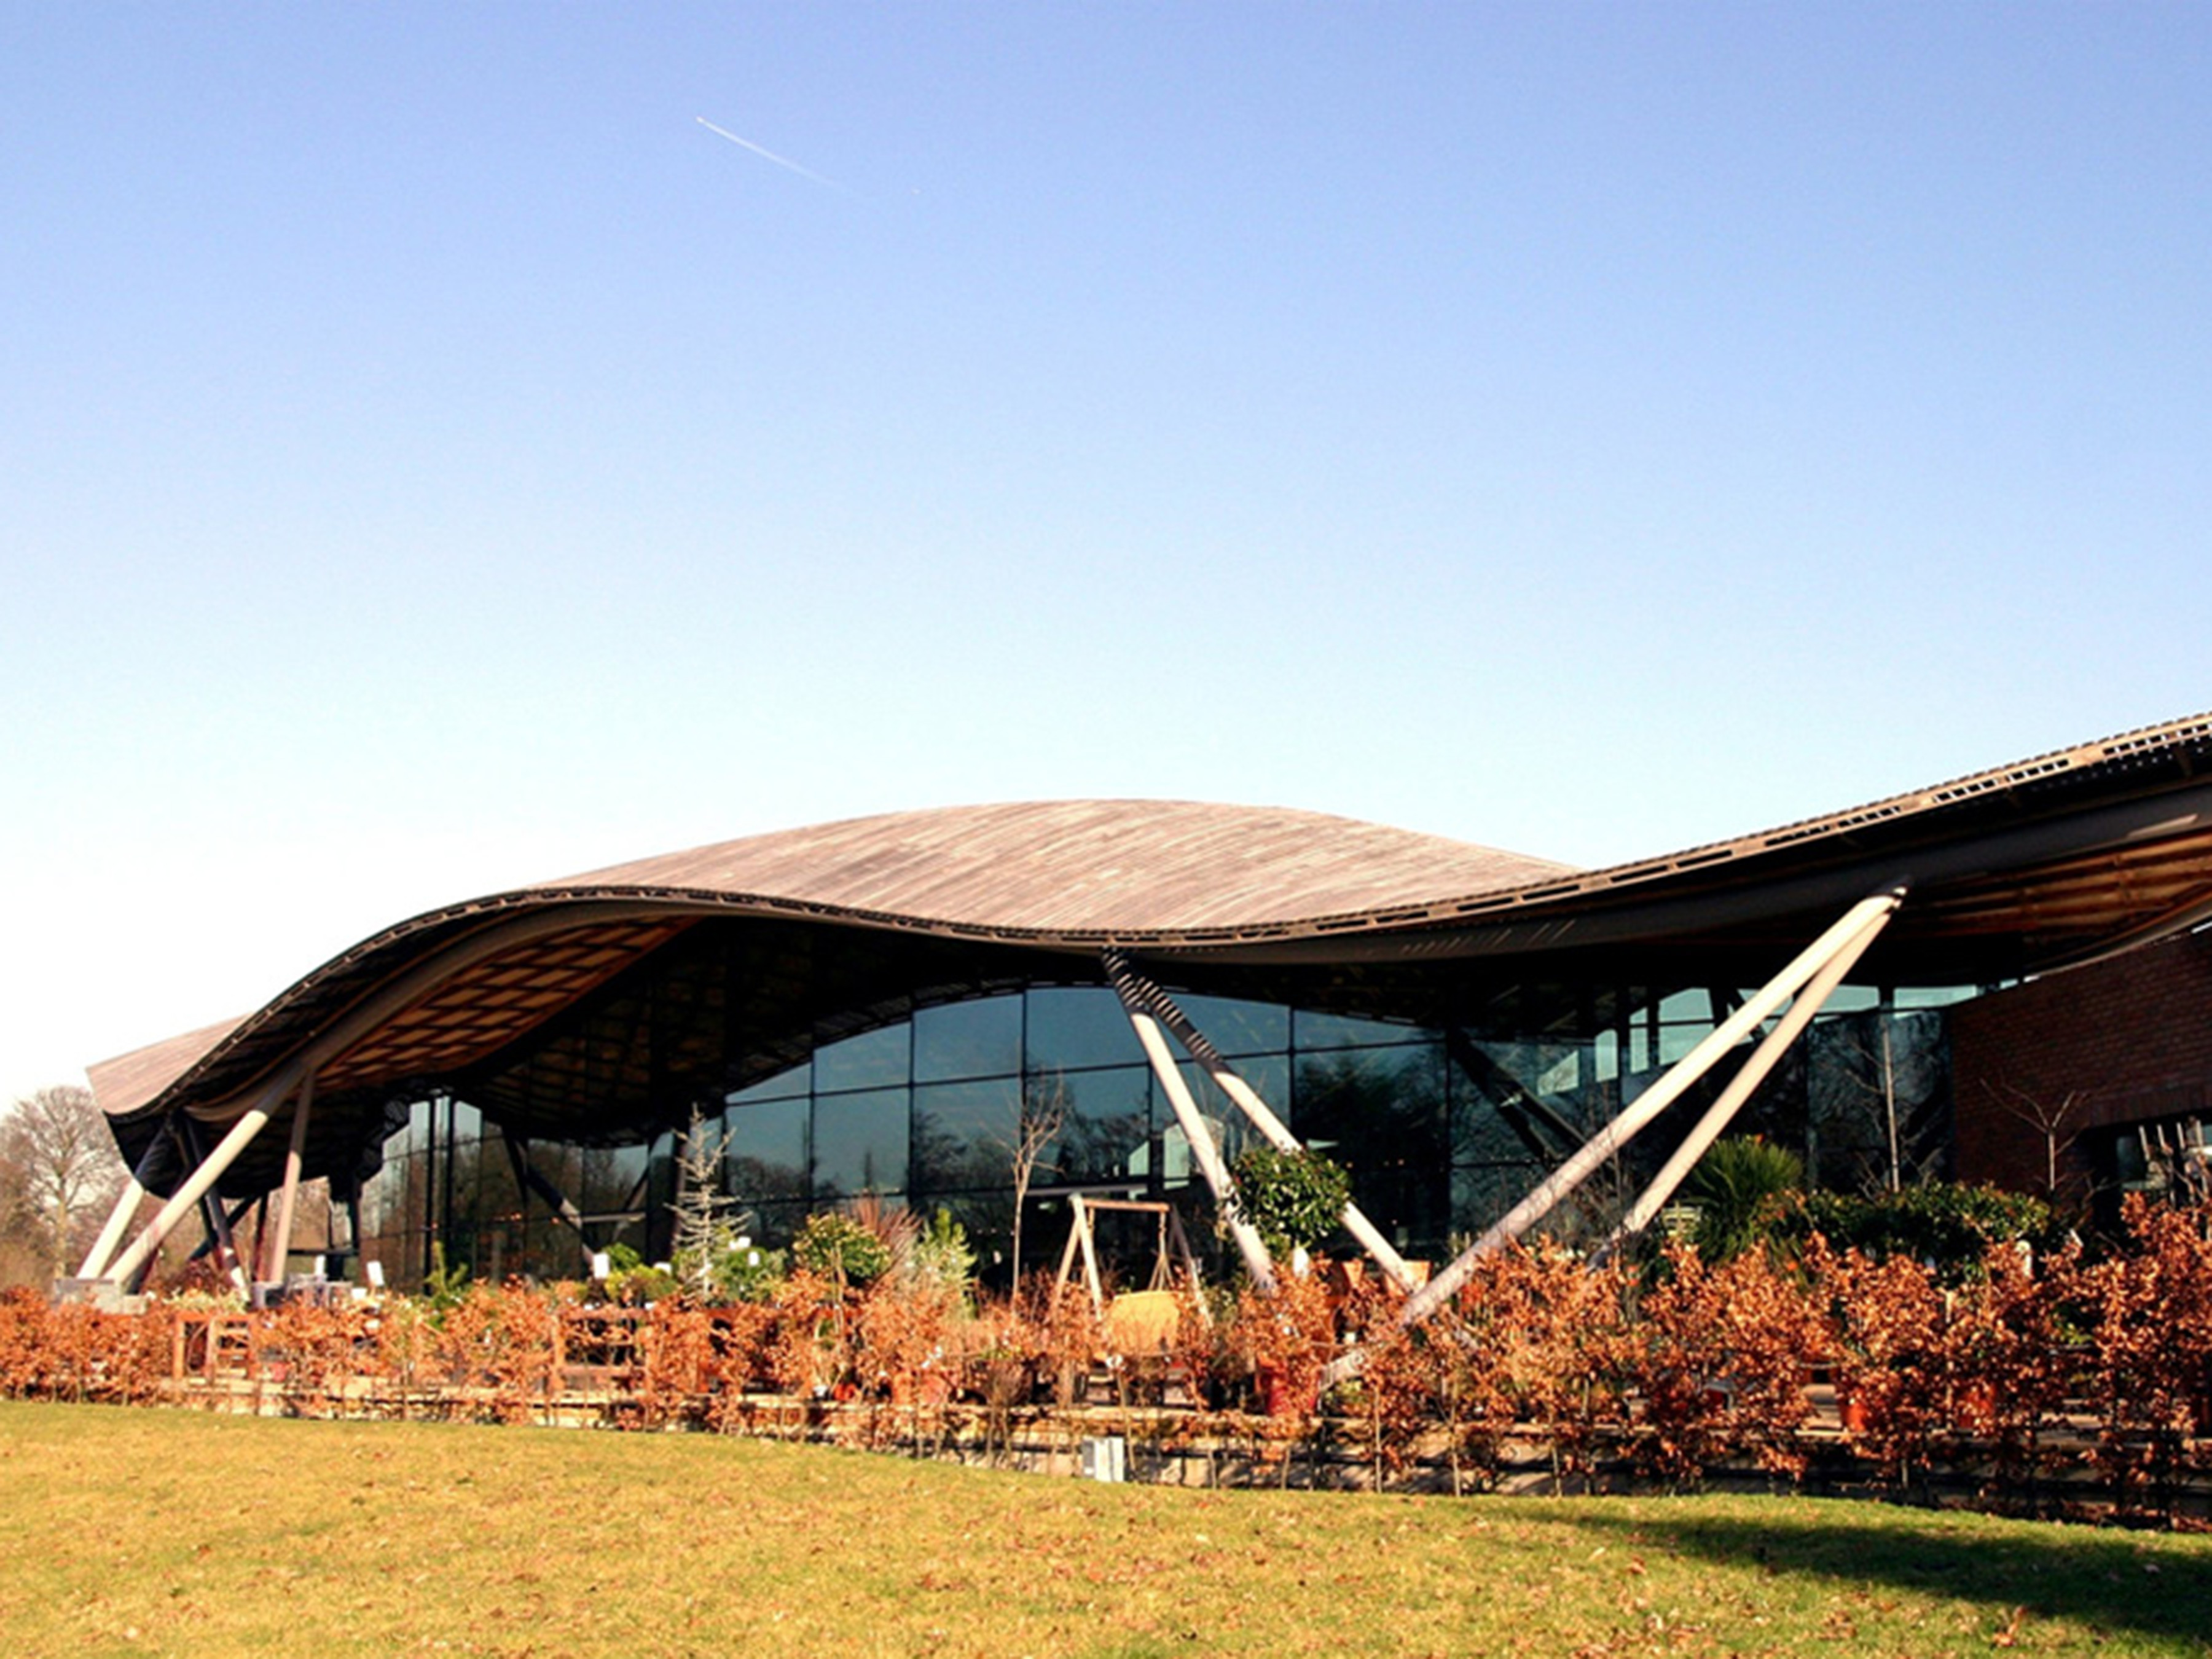
\includegraphics[width=0.48\textwidth]{savill_a.jpg}\label{fig:savill_b}}
		\vspace{10pt}
		\caption{Timber gridshell built in 2006 in Savill, England.}
		\label{fig:savill} 
\end{figure}








\clearpage


\subsubsection{The beginings}

F. Otto and its team started their experimentations in the later 60's. On of the first elastic gridshell known was made in a workshop with students in Berkeley, USA, in 1962 \cite[p.~270]{IL10}. Actually, this gridshell was not a timber gridshell but was made of twin steel rods. The technics started to expands with the construction of a timber gridshell at Essen, Germany the same year. Five years latter, in 1967, he designed two gridshells in wood that served as auditoria inside the German Pavilion for the 1967 exposition in Montreal, Canada. At this time, the IL had somme deep links with a Japanese contratctor called Seibu. This company was partly funding the research at the IL. They built an experiental structure made with tubes of hollow square section in aluminium in 1973 \cite[p.~245]{IL13}. Somme links were setted up with India too and a quite large bamboo grishell was built there in 1974 \cite[p.~304]{IL10}.


\subsubsection{Mannheil}
Tous ces projets racontent une prise en main progressive (1962-1973), aussi bien technique que constructive, de cette technologie. Ce n'est qu'à l'issu de ce cheminement fait de recherche, d'enseignement, d'expérimentation, en relisant de manière critiques les expériences réalisées, que l'IL se donne la capacité à intervenir en amont d'un processus de conception habituel, et peut pousser sa technology. C'est l'avènement du projet de Mannheim, qui marque l'histoire comme le premier gridshell élastique en bois de grande ampleur (toujours un reccords de surfafce et de portée pour cette typologie structurelle.

Dans l'IL13, on trouve également de nombreuses références à des projets étudiés qui sont restés inconstruit,  signe que F. Otto était très solicité pour ce type de struictureS.
L'expérience de Mannheim est fondatrice pour l'ingéniérie européne des structures légères. Vont s'y croiser Lehonardt (chez qui commencera) et T. Happol qui fondera plus tard sont propre bureau à Bath et concevra le reste des gridshells iconics.

EN particulier, une experience constructice très riche. Chaque nouveau séminaire, est l'occasion d'expérimenter une nouvelle méthode de mise en forme, un système d'assemble nouveau, une autre façon de contreventer, un autre matériau, une autre façon de couvrir, une forme nouvelle, etc.

\subsubsection{The desert}
Après Mannheim, il y a un creux de 25 ans. A la lecture de l'IL13 on percoit que les outils développés par F. Otto sont très avangardistes et ne peuvent pas s'"appliquer à des contextes plus courant (écomie, temps), recherhce de form sur des maquettes physiques à divers échelles, mesures élaborées par photogramétrie, calculs informatiques (les premiers pour l'époque). Celà est mis en valeur par T. Happold dans son article de Dowland, le manque d'outils numériques.

Néanmoins, cette espérience aura été formatrice pour un grand nombre d'ingénieurs ayant travayé sur ce projet, en témoigne la richesse et la diversité des articles regroupés dans l'IL13. C'est d'ailleurs le propre de tels projets : une expérience collective qui amène un saut technique, une rupture, au sein de la profession, en ce sens qu'il plante les graine pour la diffusion d'un savoir nouveau. Lorsque de tels projets commenceront à refaire surface, le B. Happold aura l'exculsivité sur la conception de la grille.

De pettis projets se font ci et là, en continuant d'explorer les système constructifs et en particuler la question de l'enveloppe. Sous l'impulsions des héritiers directes de l'expérience de Mannheim. On rappemle qu'à Mannheim, le gridshell n'était pas isolé. Par exemple un projet avec du FerroCement. Une activité effective jusque à la fin des années 70.
Puis s'en suit une vrai periode de trou. Il faut attendre 1995 pour voir réapparaitre ce qui resseble à un gridshell (tissé sur son cintre) à Hooke Par, pour la Westminster Lodge. On retrouve sur ce projet, centré sur la valorsation des thinnigs,  F. Otto et T. Happold \cite{Burton2010}. En 1998, Happold renoue avec les GS à l'occasion de la construction du Earth Center.

\subsubsection{Le renouveau}
Avec les nouveau logiciesl de calcul, celà ouvre des portes. EN 2000 Shieru Ban, assisté de F. Otto propose un gridshell en tubes de carton pour l'expo de Hannover. Le bureau sera Happold (T. H étant décédé).\cite{Ban2006}. Le projet rencontrera de nombreuses difficultrées techniques (des problèmes de creep dans les tubes nécéssitreons un renforcement par des arches un bois, qui serviront également au contreventement du gridshell en carton). Et des difficultées avec le controleur technique allememand. Donc toile PVC transparent supplémentaire par dessus la toile en papier, spécialement développé.

En 2002, c'est le grand retour du gridshell bois avec Downland \cite{Harris2003}. Confirmé avec Savill \cite{Harris2008}. Projets tous effectués avec le même charpentier Green Oak Carpentery, signe de l'importance de la sinérgie entre architecture, conception et construction. Cette équipe réitère pour l'orangerie en 2006 avec une couverture en verre. Ce sont les premiers bâtiments de ce nom, qui assurent plus qu'une couverture, mais un véritable clos couvert, avec de l'isolation.

Ces projets restent dans le ligne historiuque dessinée à Mannheim par F. Otto et ses collègues.

\subsubsection{Des pistes ouvertes}

Les méthodes numériques de Day, Barnes, Adriaenssen, Douthe, Lefevre, Tayeb
3/6/4 DOF, prise en compte de la torsion.

Le formfinding vs. grid finding (COmpas Lionel, Compas Baptise, GFFT, Compas Yannick singularité, Lina)

Les matériaux composites

Les méthodes de montage. L'inflatable(Otto, Pugnale, Quinn)

La simplification (gridshell.it => ZA, UTSA, Cluj, quaternion + Navier, Navier)

La robotisation de la production (ENPC)

Une reflexion sur l'enveloppe (booby ENPC).

Flambement (Malek, Mesnil, Lefevre)

Optimisation des sections

Description analytique de la forme (C. Williams)









\begin{landscape}%
\begin{table}[p]
\centering\small
\ra{1.3}
%\begin{fullpage}
 	\begin{tabularx}{20cm}{@{}l X l l l l l l r@{}}
	\toprule
%		&				&		&				&			&			& \multicolumn{2}{c}{Project Team}						& 	\\ \cmidrule(l){7-8}
 	N	& Nickname		& Year	& City			& Country		& Type		& Architecte 			& Enginneer			& Ref \\ 
	\midrule
	1 	& Berkeley		& 1962	& Berkeley		& USA		& Prototype	& F. Otto	 			& F. Otto				& \cite{IL10} \\
	2 	& Essen			& 1962	& Essen			& Germany	& Pavilion		& F. Otto	 			& F. Otto				& \cite{IL10} \\
	3 	& German Pavillion	& 1967	& Montreal		& Canada		& Pavilion		& F. Otto	 			& F. Otto				& \cite{IL10} \\
	4 	& Seibu			& 1973	& Tokyo			& Japan		& Prototype	& K. Matsushita	 		& T. Shirayanagi		& \cite[p.~245]{IL13} \\
	5 	& Ahmedabad		& 1976	& Ahmedabad		& India		& Building		& G. Sarabhai 			& G. Ramaswamy		& \cite[p.~249]{IL13} \\
	6 	& Bamboo			& 1976	& London			& England		& Workshop	& J. Park 				& B. Oleiko			& \cite{IL13} \\

	7 	& Mexico			& 1973	& Tokyo			& Japan		& Protorype	& J. Hennicke			& J. Hennicke			& \cite{IL13} \\
	8 	& Mexico			& 1973	& Tokyo			& Japan		& Workshop	& J. Hennicke			& J. Hennicke			& \cite{IL13} \\

	9 	& Mexico			& 1977	& Zitacuaro		& Mexico		& House		& F. Montero			& F. Montero			& \cite{IL13} \\

	\midrule
	10 	& Mannheim		& 1975	& Mannheim		& Germany	& Building		& C. Mutschler 	 		& Arup + F. Otto  		& \cite{IL13} \\
	11 	& Japan Pavilion	& 2000	& Hannover		& Germany	& Pavilion		& S. Ban + F. Otto		& Buro Happold 		& \cite{} \\
	12 	& Downland		& 2002	& Singleton		& England		& Building		& E. Cullinan	 		& Buro Happold		& \cite{Harris2003} \\
	13 	& Savill			& 2006	& Englefield		& England		& Building		& G. Howells			& Buro Happold		& \cite{Harris2008} \\
	14 	& Chiddingstone	& 2007	& Chiddingstone	& England		& Canopy		& P. Hulbert			& Buro Happold		& \cite{} \\
	
	\bottomrule
 	\end{tabularx}
\captionof{table}[Key numbers]{Key numbers.}
%\end{fullpage}
\end{table}
\end{landscape}%



\begin{landscape}%
\begin{table}[p]
\centering\small
\ra{1.3}
%\begin{fullpage}
 	\begin{tabular}{@{}llll  lllllr@{}}
	\toprule
%    &         & 	          & Type & City & Country & Architecte & Engineer & Page & Citation \\
N & Year & Nickname & Type & City & Country & Architecte & Engineer & Page & Citation\\
1 & 1962 & Experimental structure  & Workshop & Berkeley & USA & Students & F. Otto & p.~270 & \cite{IL10}\\
2 & 1962 & Exhibition pavilion & Pavilion & Essen & Germany & F. Otto & F. Otto & p.~272 & \cite{IL10}\\
3 & 1967 & German Pavilion & Pavilion & Montreal & Canada & F. Otto & Lehonardt & p.~274 & \cite{IL10}\\
4 & 1973 & Seibu & Experiment & Tokyo & Japan & IL & IL & p.~245 & \cite{IL13}\\
5 & 1974 & Basket shell & Experiment & Amehabad & India & G. Sarabhai & IL & p.~304 & \cite{IL10}\\
6 & 1974 & Experimental structure  & Experiment & London & England & Students & Arup + IL & p.~306 & \cite{IL10}\\
7 & 1975 & Mannheim Multihalle & Building & Mannheim & Germany & C. Mutshler & Arup + IL & p.~308 & \cite{IL10}\\
8 & 1973 & Ferrocement gridshell & Building & Ahmedabad & India & G. Sarabhai & G. Ramaswamy + IL & p.~248 & \cite{IL13}\\
9 & 1976 & AA Bamboo Latice Shell & Workshop & London & England & Students & J. Park + B. Oleiko & p.~255 & \cite{IL13}\\
10 & 1976 & Test structure of a gridshell & Experiment & Stuttgart & Germany & Students & J. Hennicke & p.~298 & \cite{IL10}\\
11 & 1977 & Small Pavilion & Workshop & Mexico City & Mexico & Students & J. Hennicke & p.~258 & \cite{IL13}\\
11 & 1977 & Small Greenhouse & Workshop & Zitacuaro & Mexico & Students & F. Montero & p.~260 & \cite{IL13}\\
12 & 1977 & Experimental structure & Workshop & Mexico City & Mexico & Students & F. Montero & p.~270 & \cite{IL13}\\
13 & 1977 & Experimental structure & Workshop & Mexico City & Mexico & Students & F. Montero & p.~270 & \cite{IL13}\\
14 & 1995 & Westminster Lodge & Building & Dorset & England & E. Cullinan & F. Otto + Happold & p.~90 & \cite{Burton2010}\\
15 & 1998 & Earth Center & Building & Doncaster & England & Grant & Happold &  & \\
16 & 2000 & Japan Pavilion & Pavilion & Hannover & Germany & S. Ban + F. Otto & Happold &  & \cite{Ban2006}\\
17 & 2002 & Downland & Building & Downland & England & E. Cullinan & Happold + C. William &  & \cite{Harris2003}\\
18 & 2003 & Life Science Centre Trust & Building & Pishwanton & England &  &  &  & \\
19 & 2006 & Savill & Building & Savill & England & G. Howells & Happold + C. William &  & \cite{Harris2008}\\
20 & 2007 & Chiddingstone Orangery & Roofing & Kent & England & P. Hulbert & Happold &  & \\
21 & 2007 & ENPC & Experiment & Noisy-Champs & France & Navier & Navier &  & \cite{Douthe2006}\\
22 & 2011 & Solidays & Pavilion & Paris & France & ENPC & Navier + T/E/S/S &  & \cite{Baverel2012}\\
23 & 2012 & Toledo & Workshop & Naples & Italy & gridshell.it & B. D'Amico &  & \cite{DAmico2014}\\
24 & 2013 & Créteil & Building & Créteil & France & T/E/S/S & T/E/S/S + Navier &  & \cite{DuPeloux2016}\\
25 & 2014 & Toledo 2.0 & Workshop & Naples & Italy & gridshell.it & B. D'Amico &  & \cite{DAmico2015a}\\
26 & 2016 & JPO & Pavilion & Toulouse & France & Quaternion & Navier + Terrell &  & \\
27 & 2016 & FAV & Pavilion & Montpellier & France & Quaternion & Navier + Terrell &  & \\
28 & 2016 & CLC & Workshop & Noisy-Champs & France & ENPC & Navier &  & \\
27 & 2016 & Trondheim & Workshop & Trondheim & Norway & Students & NTNU &  & \cite{Mork2016}\\
 	\end{tabular}
\captionof{table}[Key numbers]{Key numbers.}
%\end{fullpage}
\end{table}
\end{landscape}%


\clearpage

\begin{landscape}%
\begin{table}[p]
\centering
\ra{1.1}
%\begin{fullpage}
 	\begin{tabularx}{20cm}{@{}lll rrrXXX@{}}
	\toprule
		&			& \multicolumn{2}{c}{Project} 			& \multicolumn{3}{c}{Structure}	 	\\
	\cmidrule(l){3-4} \cmidrule(l){5-7}
 	Year & Nickname 	& Country		& Duration			& Material 	& Layer	& Pitch		\\ 
	\midrule
	1975	& Mannheim	& Germany	& LT					& hemlock	 	& double	& \SI{0.5}{m}	\\	
	\bottomrule
 	\end{tabularx}
\captionof{table}[Key numbers]{Key numbers.}
%\end{fullpage}
\end{table}
\end{landscape}%




\clearpage

\footnote{German pavilion 1967 : \url{https://www.youtube.com/watch?v=Z0mtFMoseUk}}
\footnote{German pavilion 1967 : \url{http://www.uncubemagazine.com/magazine-33-15508949.html/page1}}



\section{Building free-forms}
\subsection{Non-standard forms}
\subsection{Importance of free-forms in modern architecture}
\subsection{Canonical approaches to build free-forms}
\subsection{Main challenges}

\section{Gridshell structure : definition and classification}
\subsection{Historic overview}
\subsection{Rigid gridshell}
\subsection{Elastic gridshell}

The invention of the gridshell concept is commonly attributed to Frei Otto, a German architect who devoted several years to gridshells. In 1975 he achieved the famous \emph{Mannheim Multihalle} \cite{Happold1975}, a wooden shell of 7500~m\textsuperscript{2}, in collaboration with the engineer Edmund Happold (Arup).
Literally, the word \textquote{gridshell} refers to grids behaving like shells~: from a mechanical point of view that means stresses acting on the structure are mainly transmitted through compression and traction. These structures can cross large-span with very little material.

However, according to the historic evolution of the concept, characterizing a gridshell as the combination of a structural concept -- a grid behaving like a shell -- and a specific construction process -- using the bending flexibility of the material -- seems to be more accurate. The Mannheim project (in which a wooden regular and planar grid, lacking shear stiffness, is elastically deformed up to a targeted shape with the help of stays, and then braced and covered) is regarded as the starting point of this new concept.

The Mannheim project is regarded as the starting point of this new concept for which a wooden regular and planar grid, lacking shear stiffness, is elastically deformed up to a targeted shape with the help of stays, and then braced and covered.
This type of gridshell, known as elastic gridshell, offers a very elegant manner to materialize freeform shapes from an initially flat and regular grid, which obviously has many practical benefits: planar geometry, standard connection nodes, standard profiles and so on.


\begin{figure}[h]
		\captionsetup[subfloat]{captionskip=10pt}
		\subfloat[][Forum Café, Solidays (2011).]{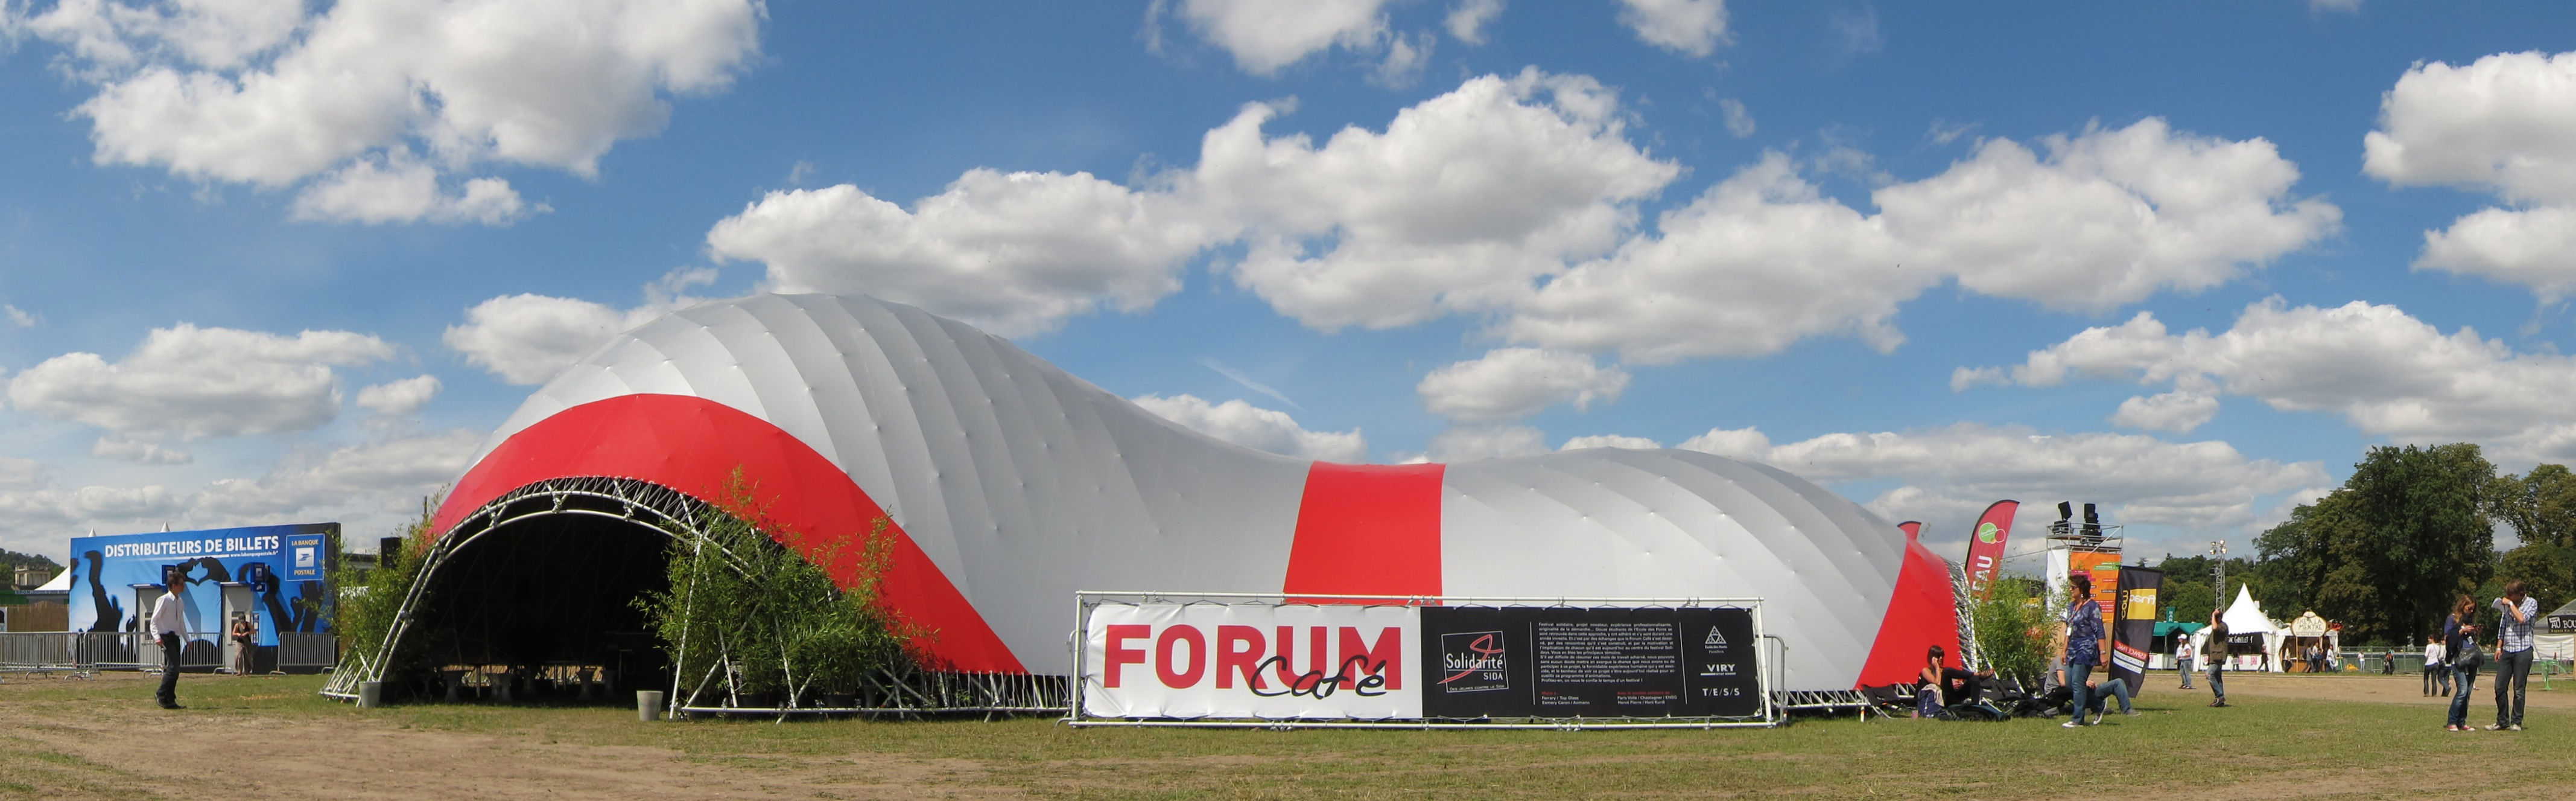
\includegraphics[width=1\textwidth]{solidays.jpg}\label{fig:solidays}}\\
		\subfloat[][Prototype (2007).]{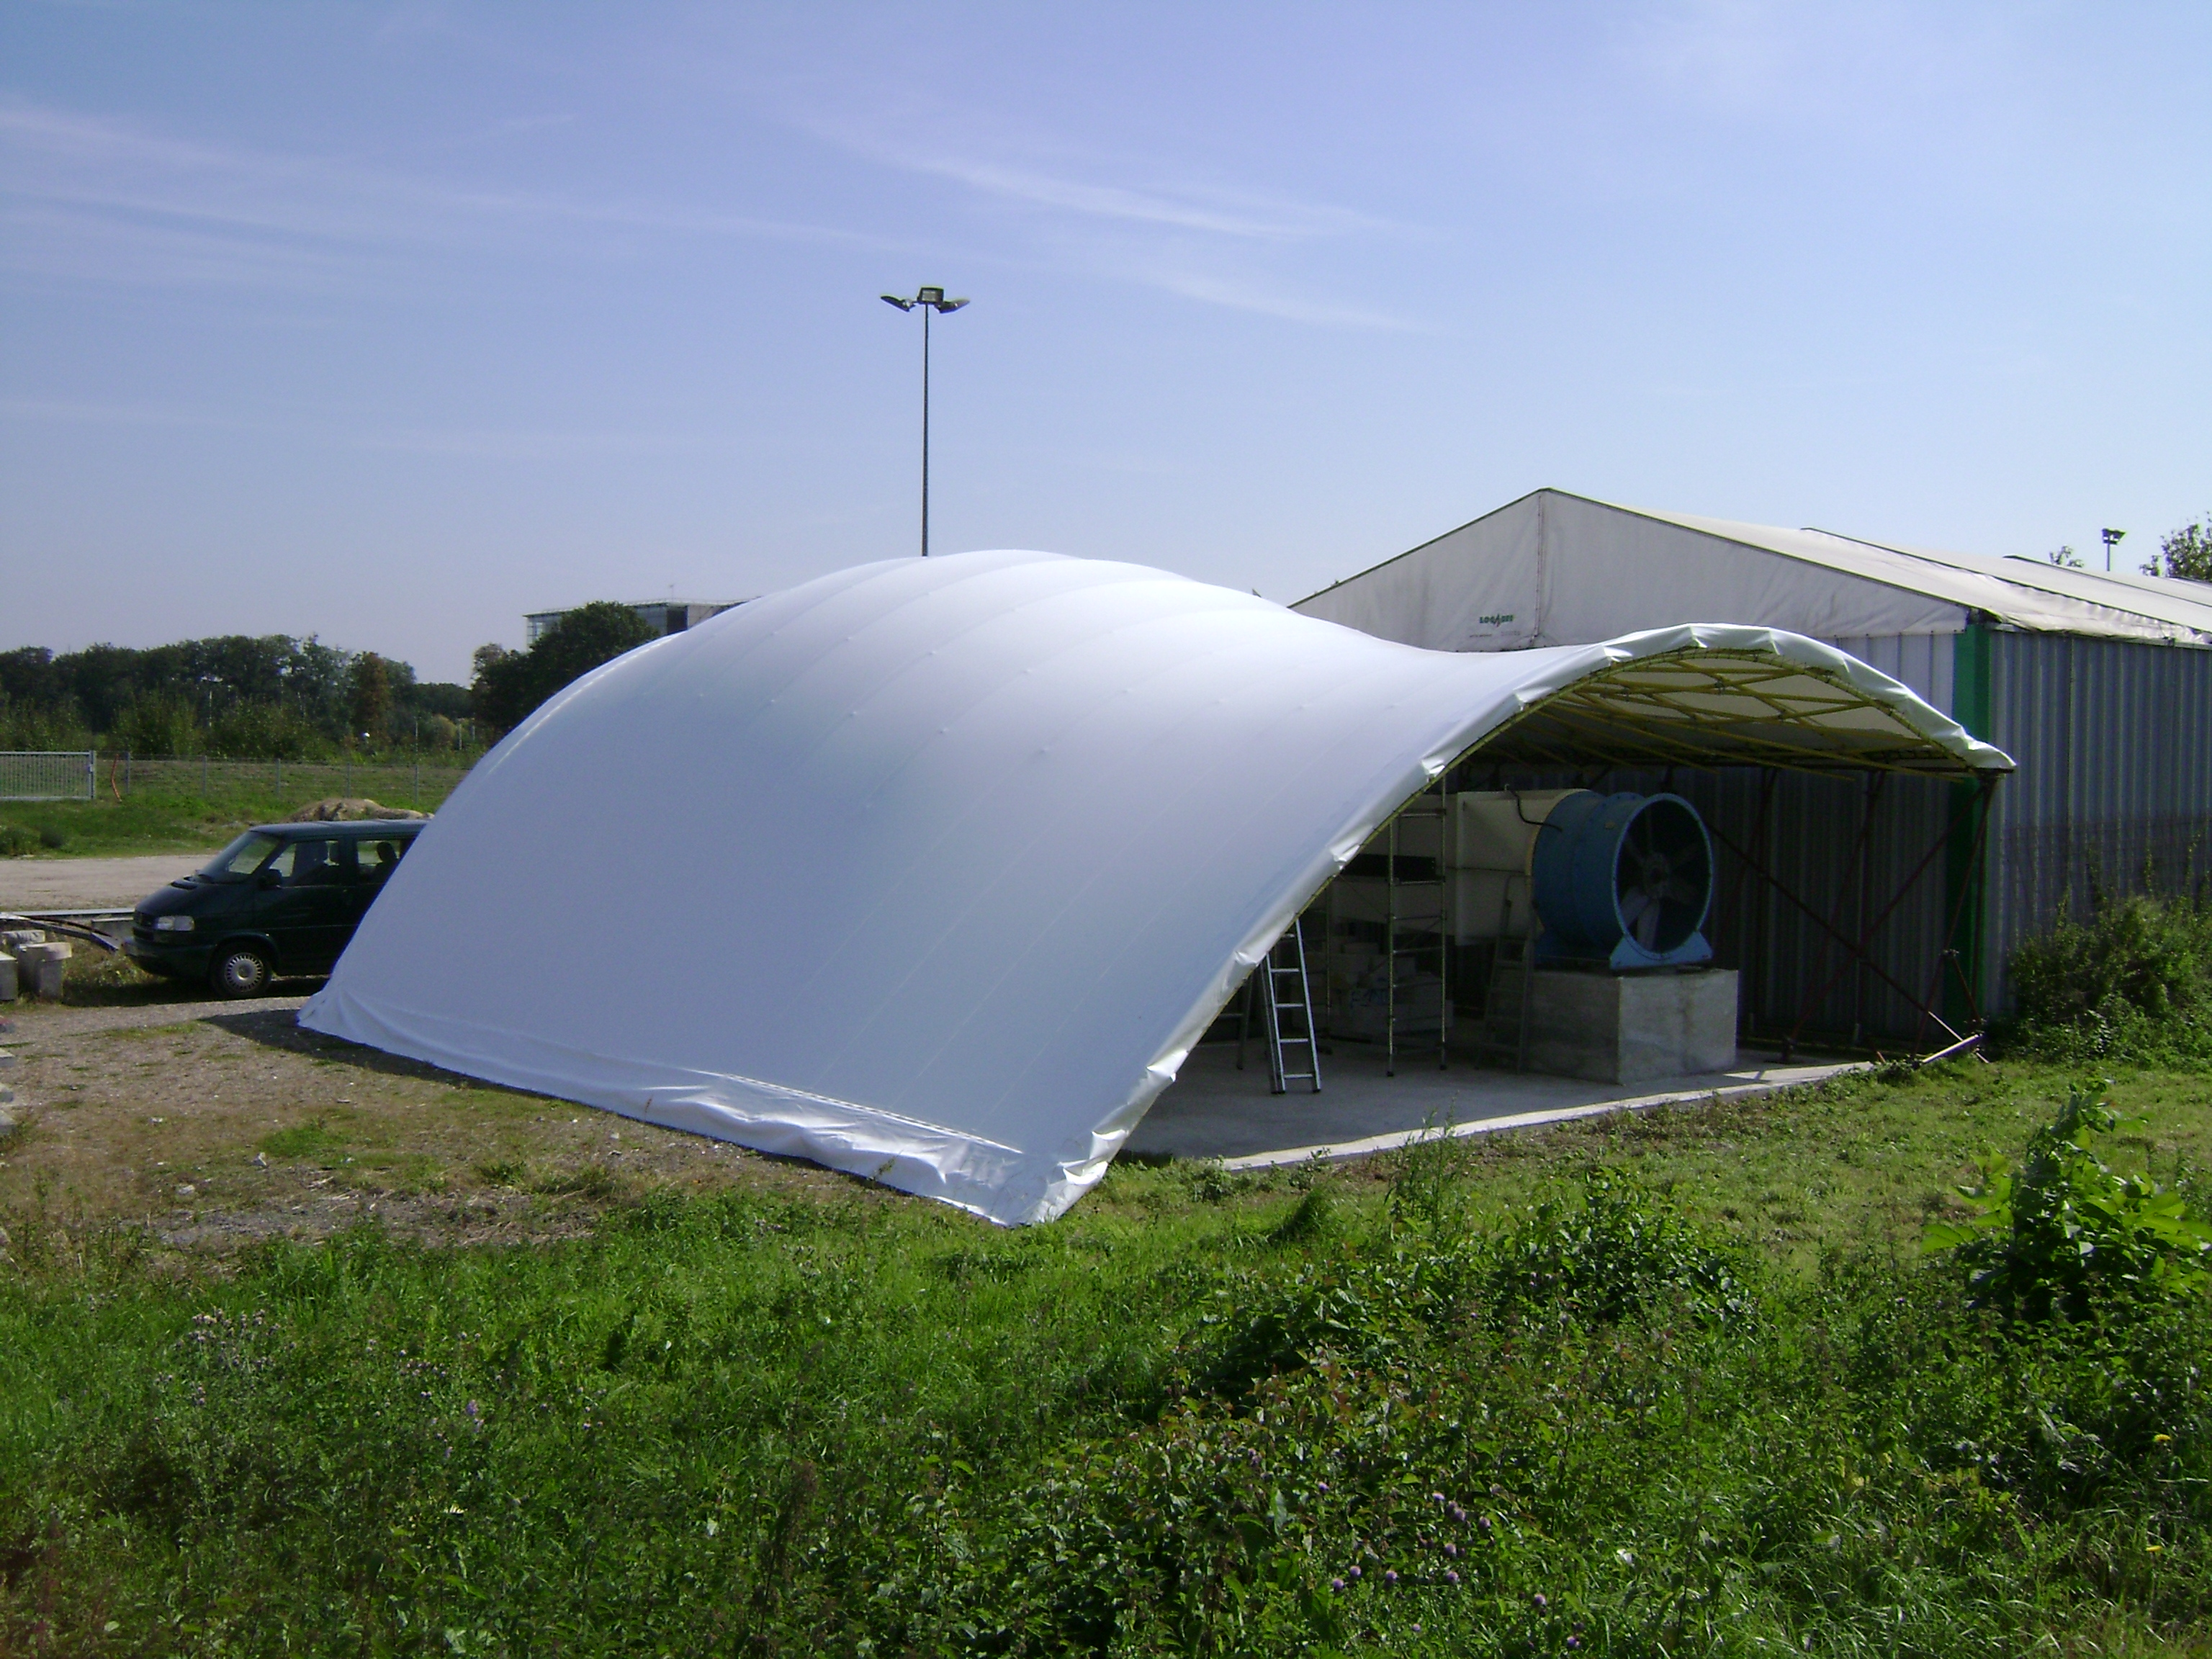
\includegraphics[width=0.48\textwidth]{proto_a.jpg}\label{fig:proto_a}}
		\hspace*{\fill}
		\subfloat[][Prototype (2008).]{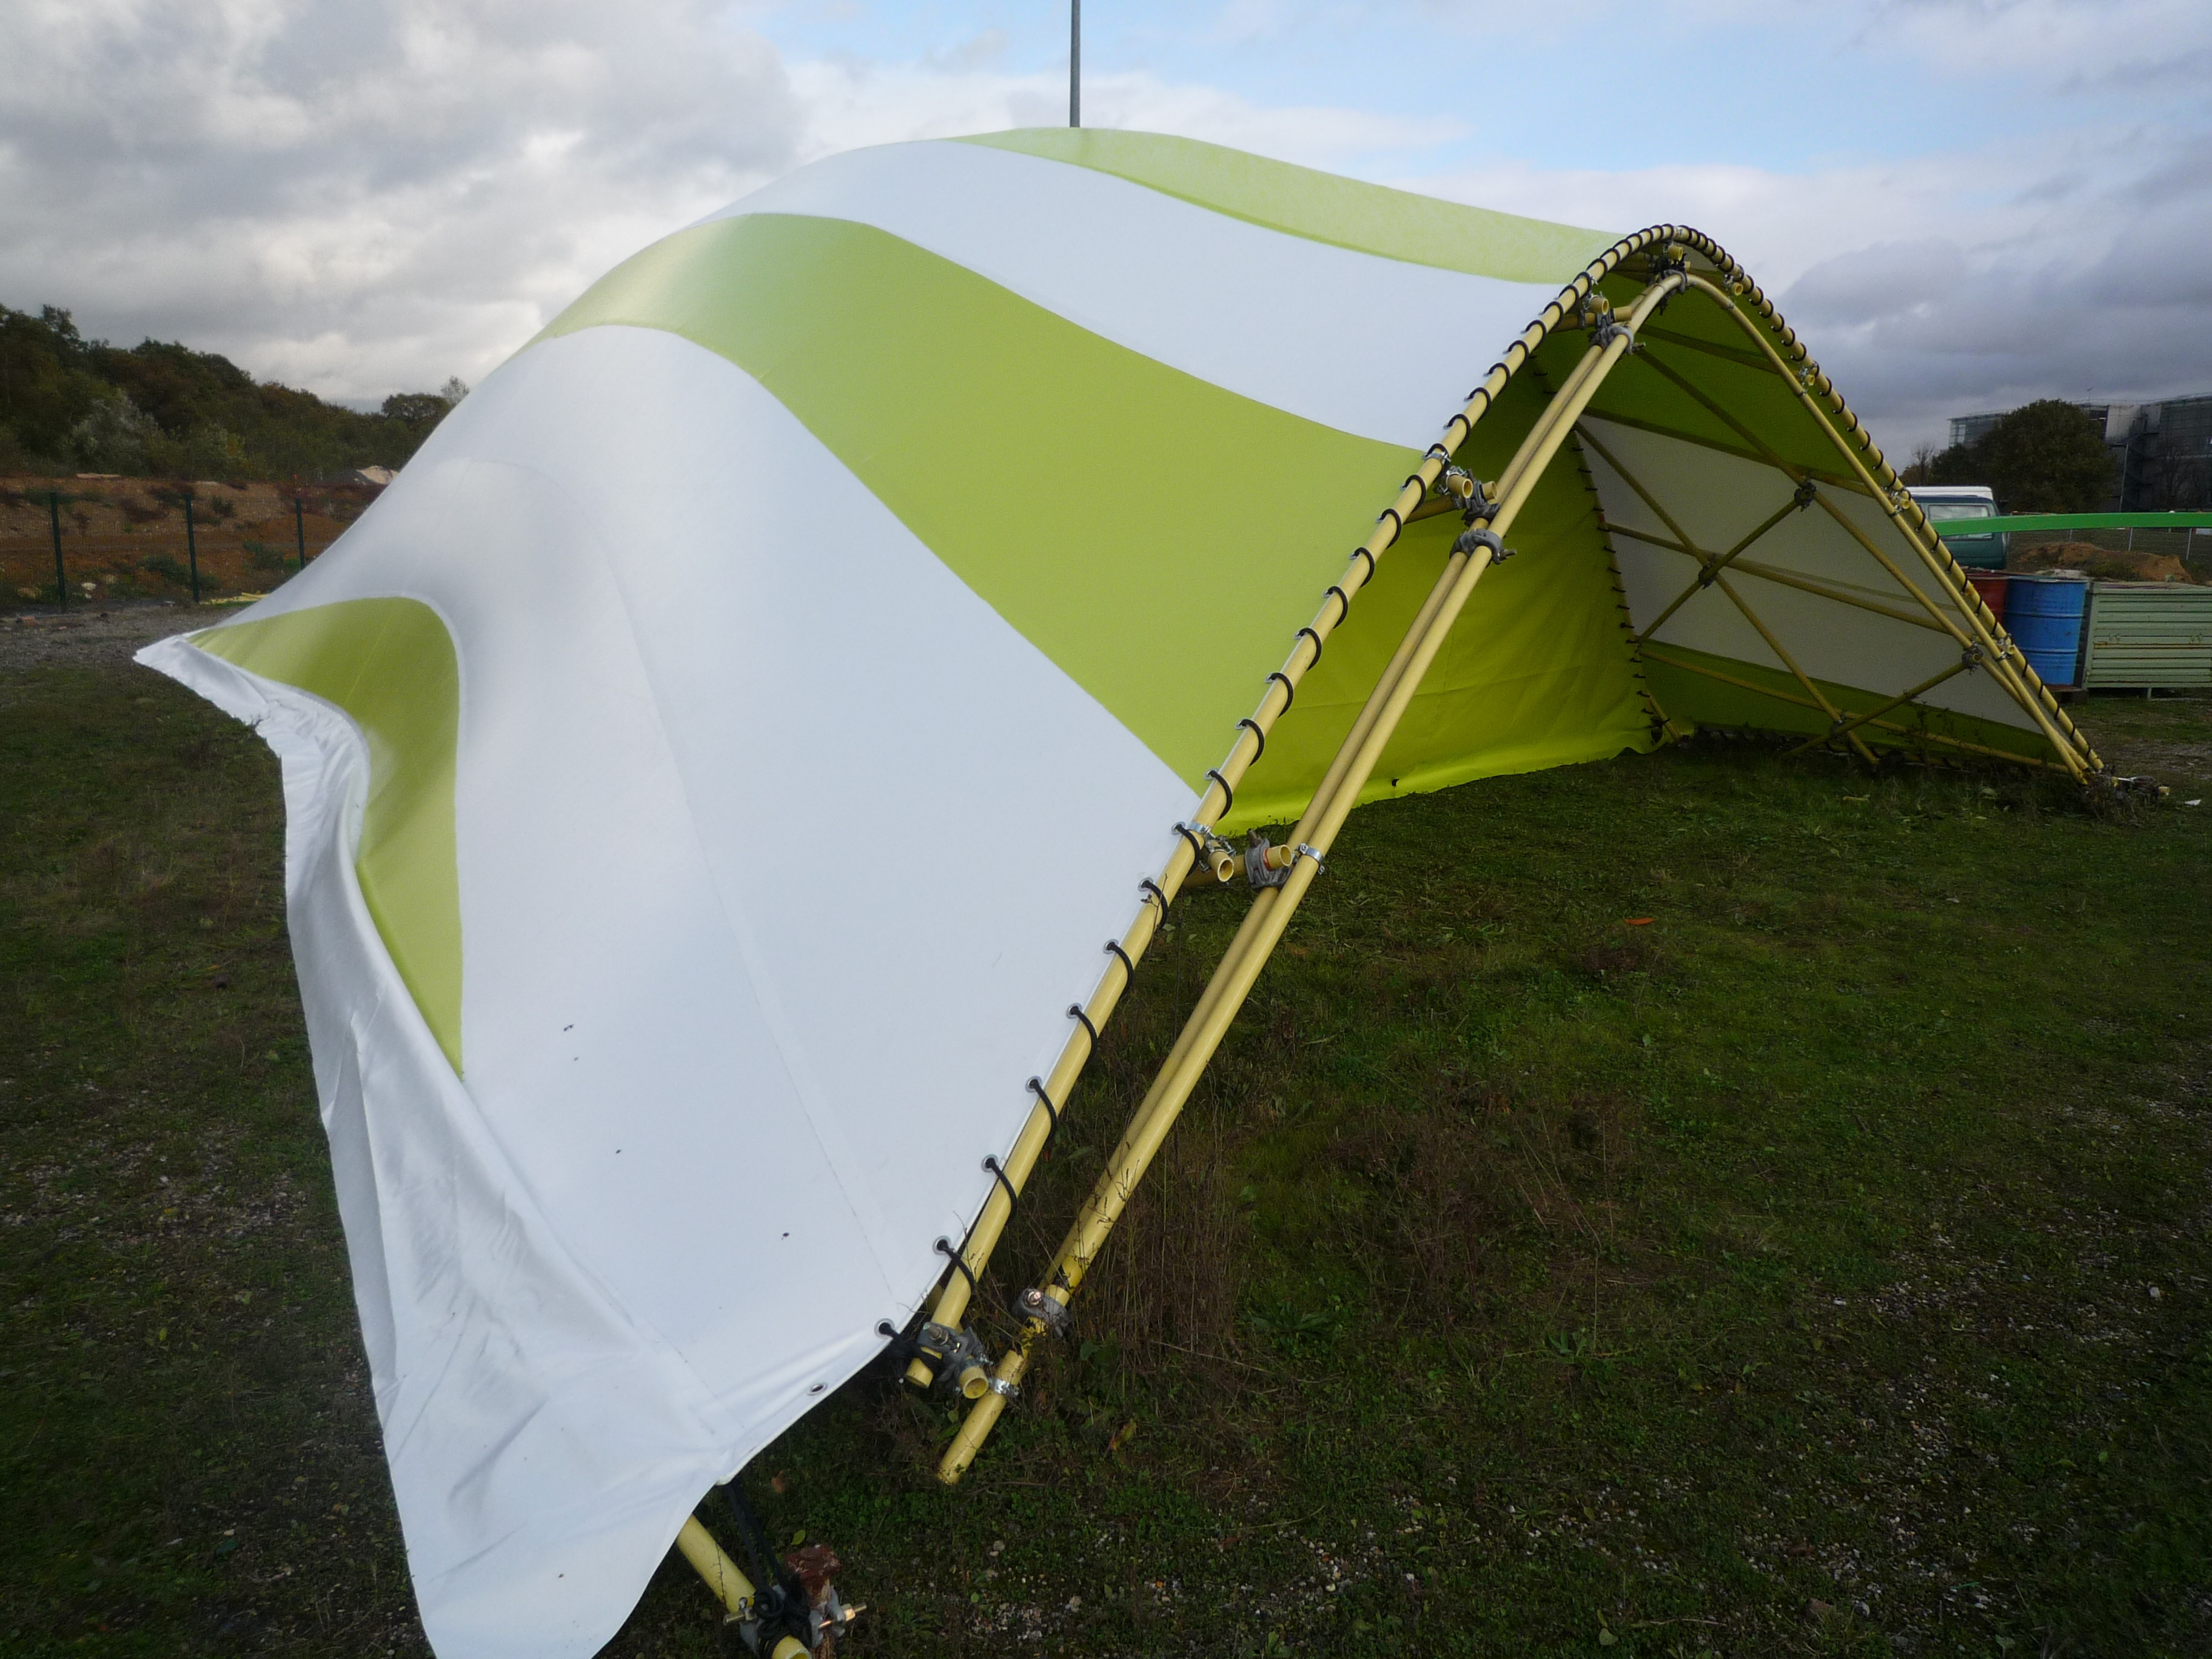
\includegraphics[width=0.48\textwidth]{proto_b.jpg}\label{fig:proto_b}}
		%
		\vspace{10pt}
		\caption{Prototypes and projects of GFRP elastic gridshells.}
		\label{fig:proto}    
\end{figure}

\begin{figure}[p]
	\begin{fullpage}
		\captionsetup[subfloat]{captionskip=10pt}
     		\centering
     		%
		\subfloat[][Mannheim (1975).]{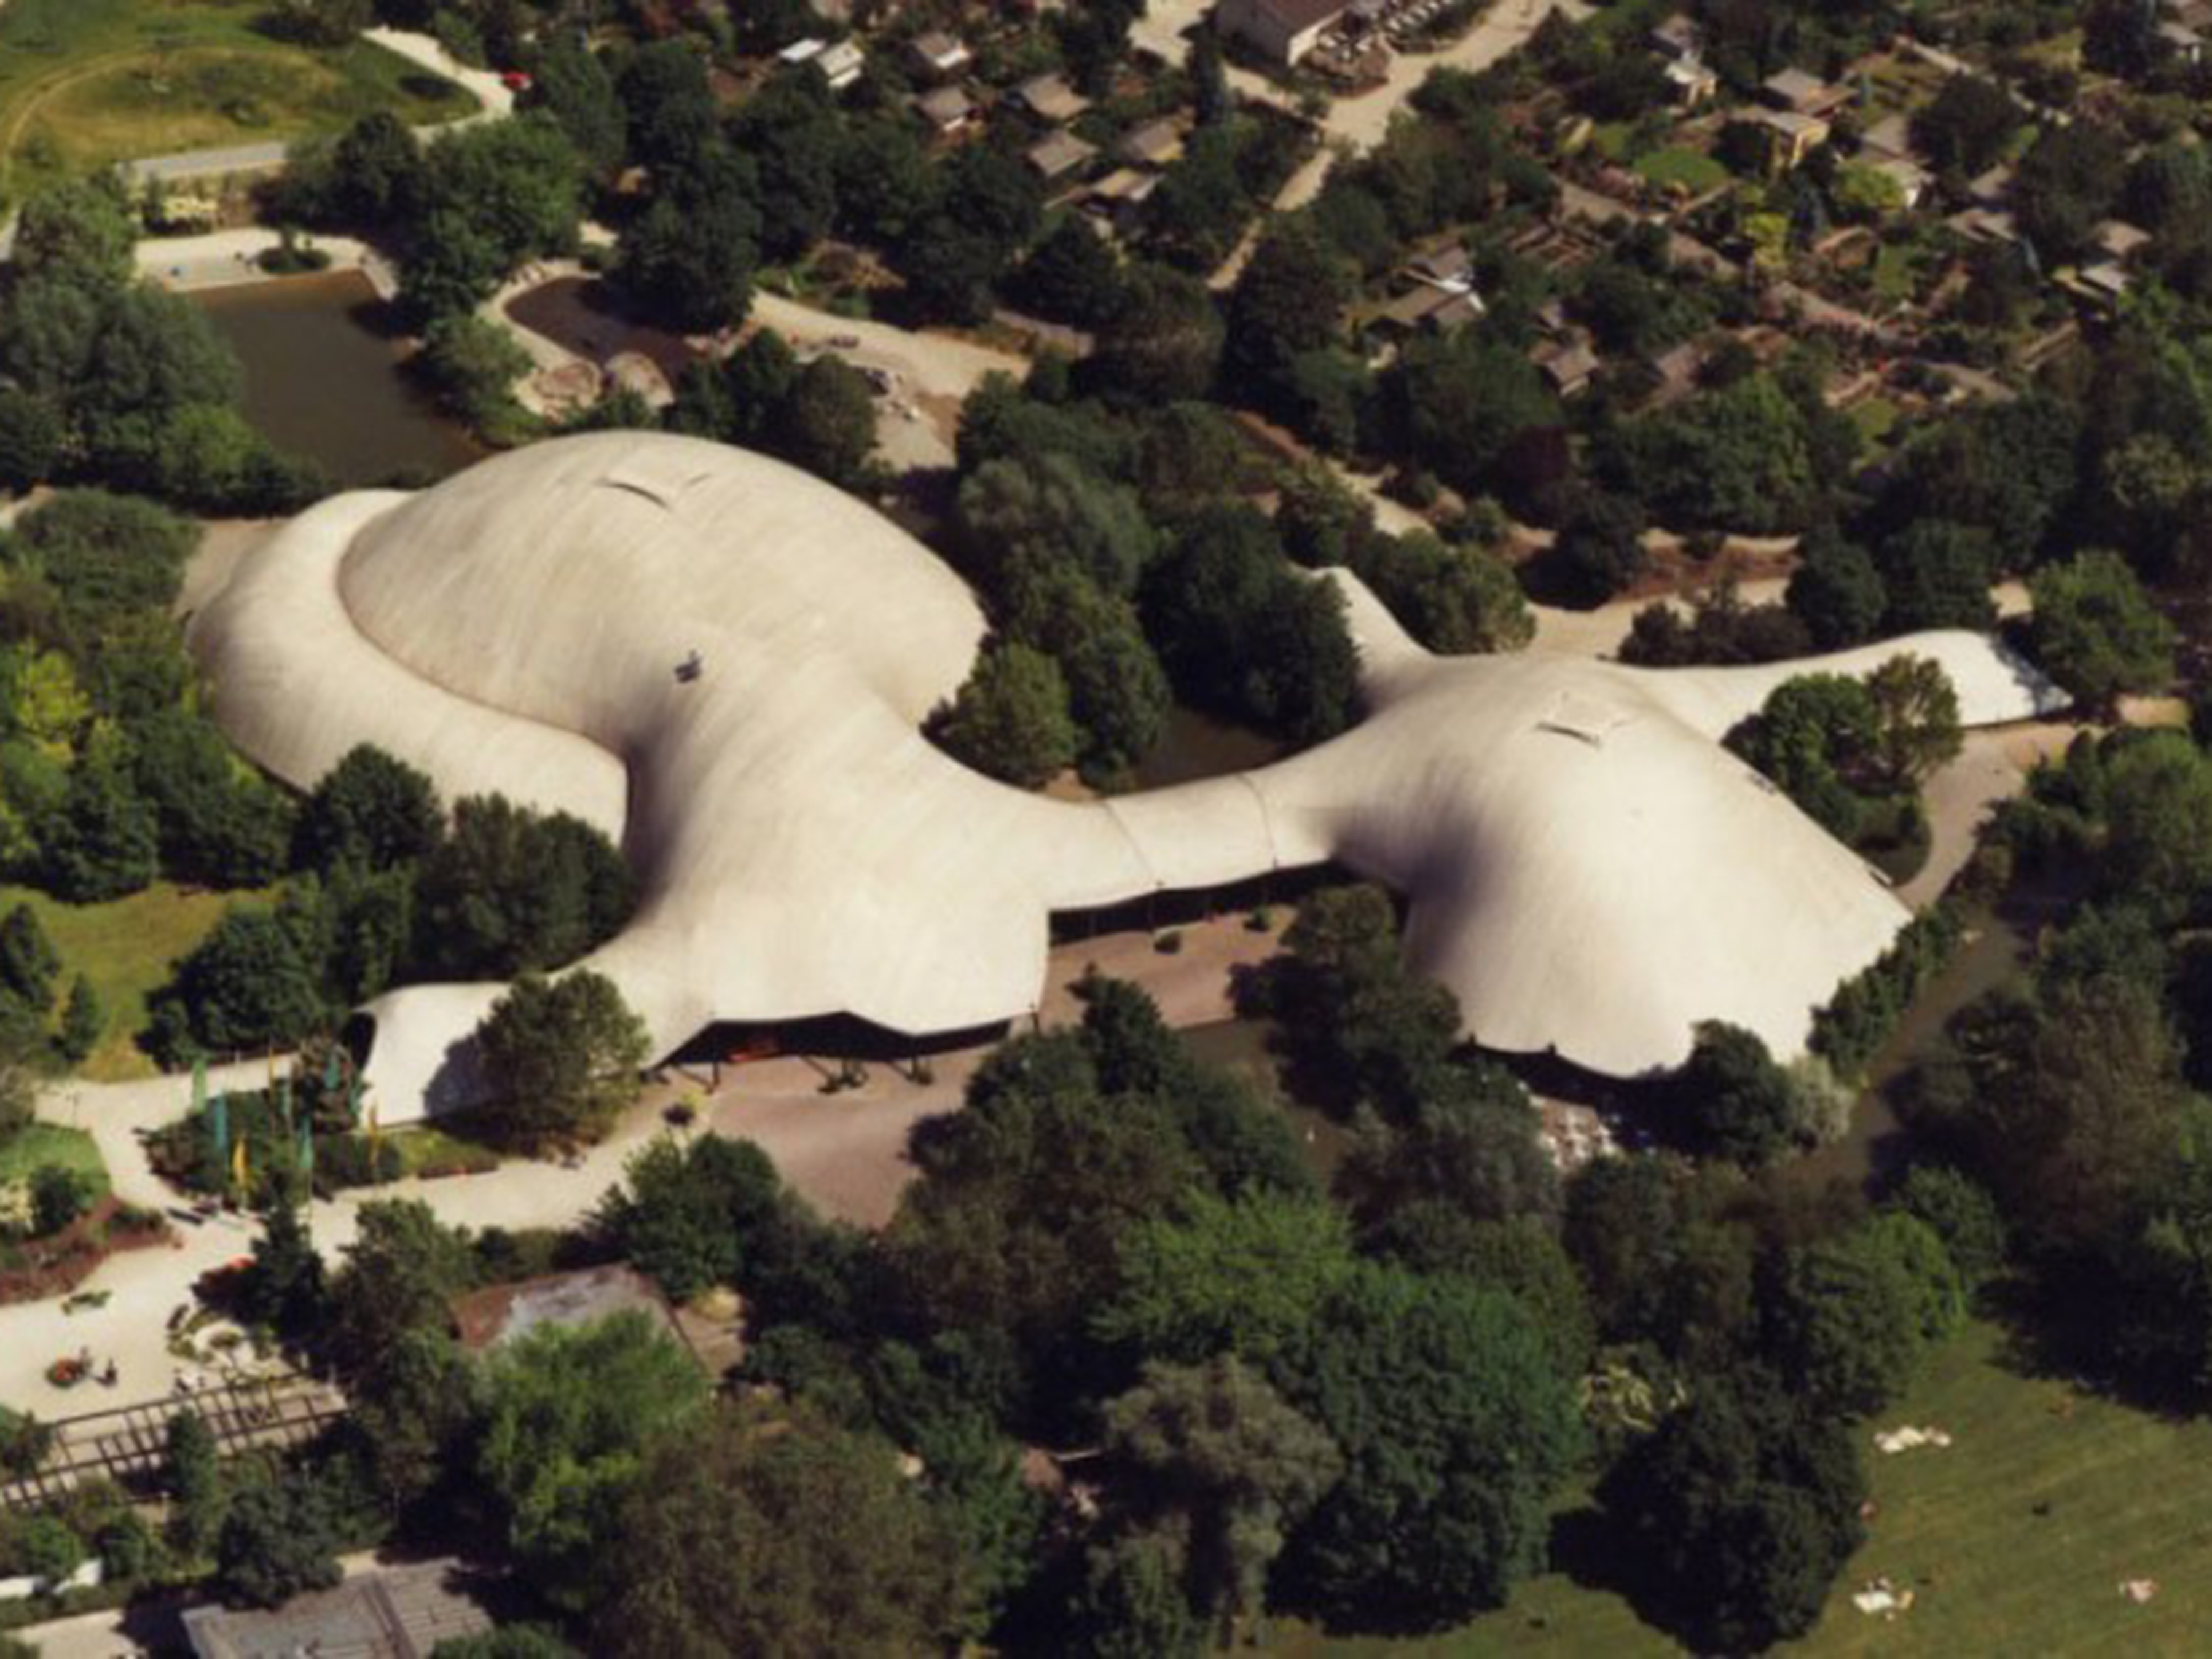
\includegraphics[width=0.48\textwidth]{mannheim_a.jpg}\label{fig:mannheim_a}}
		\hspace*{\fill}
		\subfloat[][Mannheim (1975).]{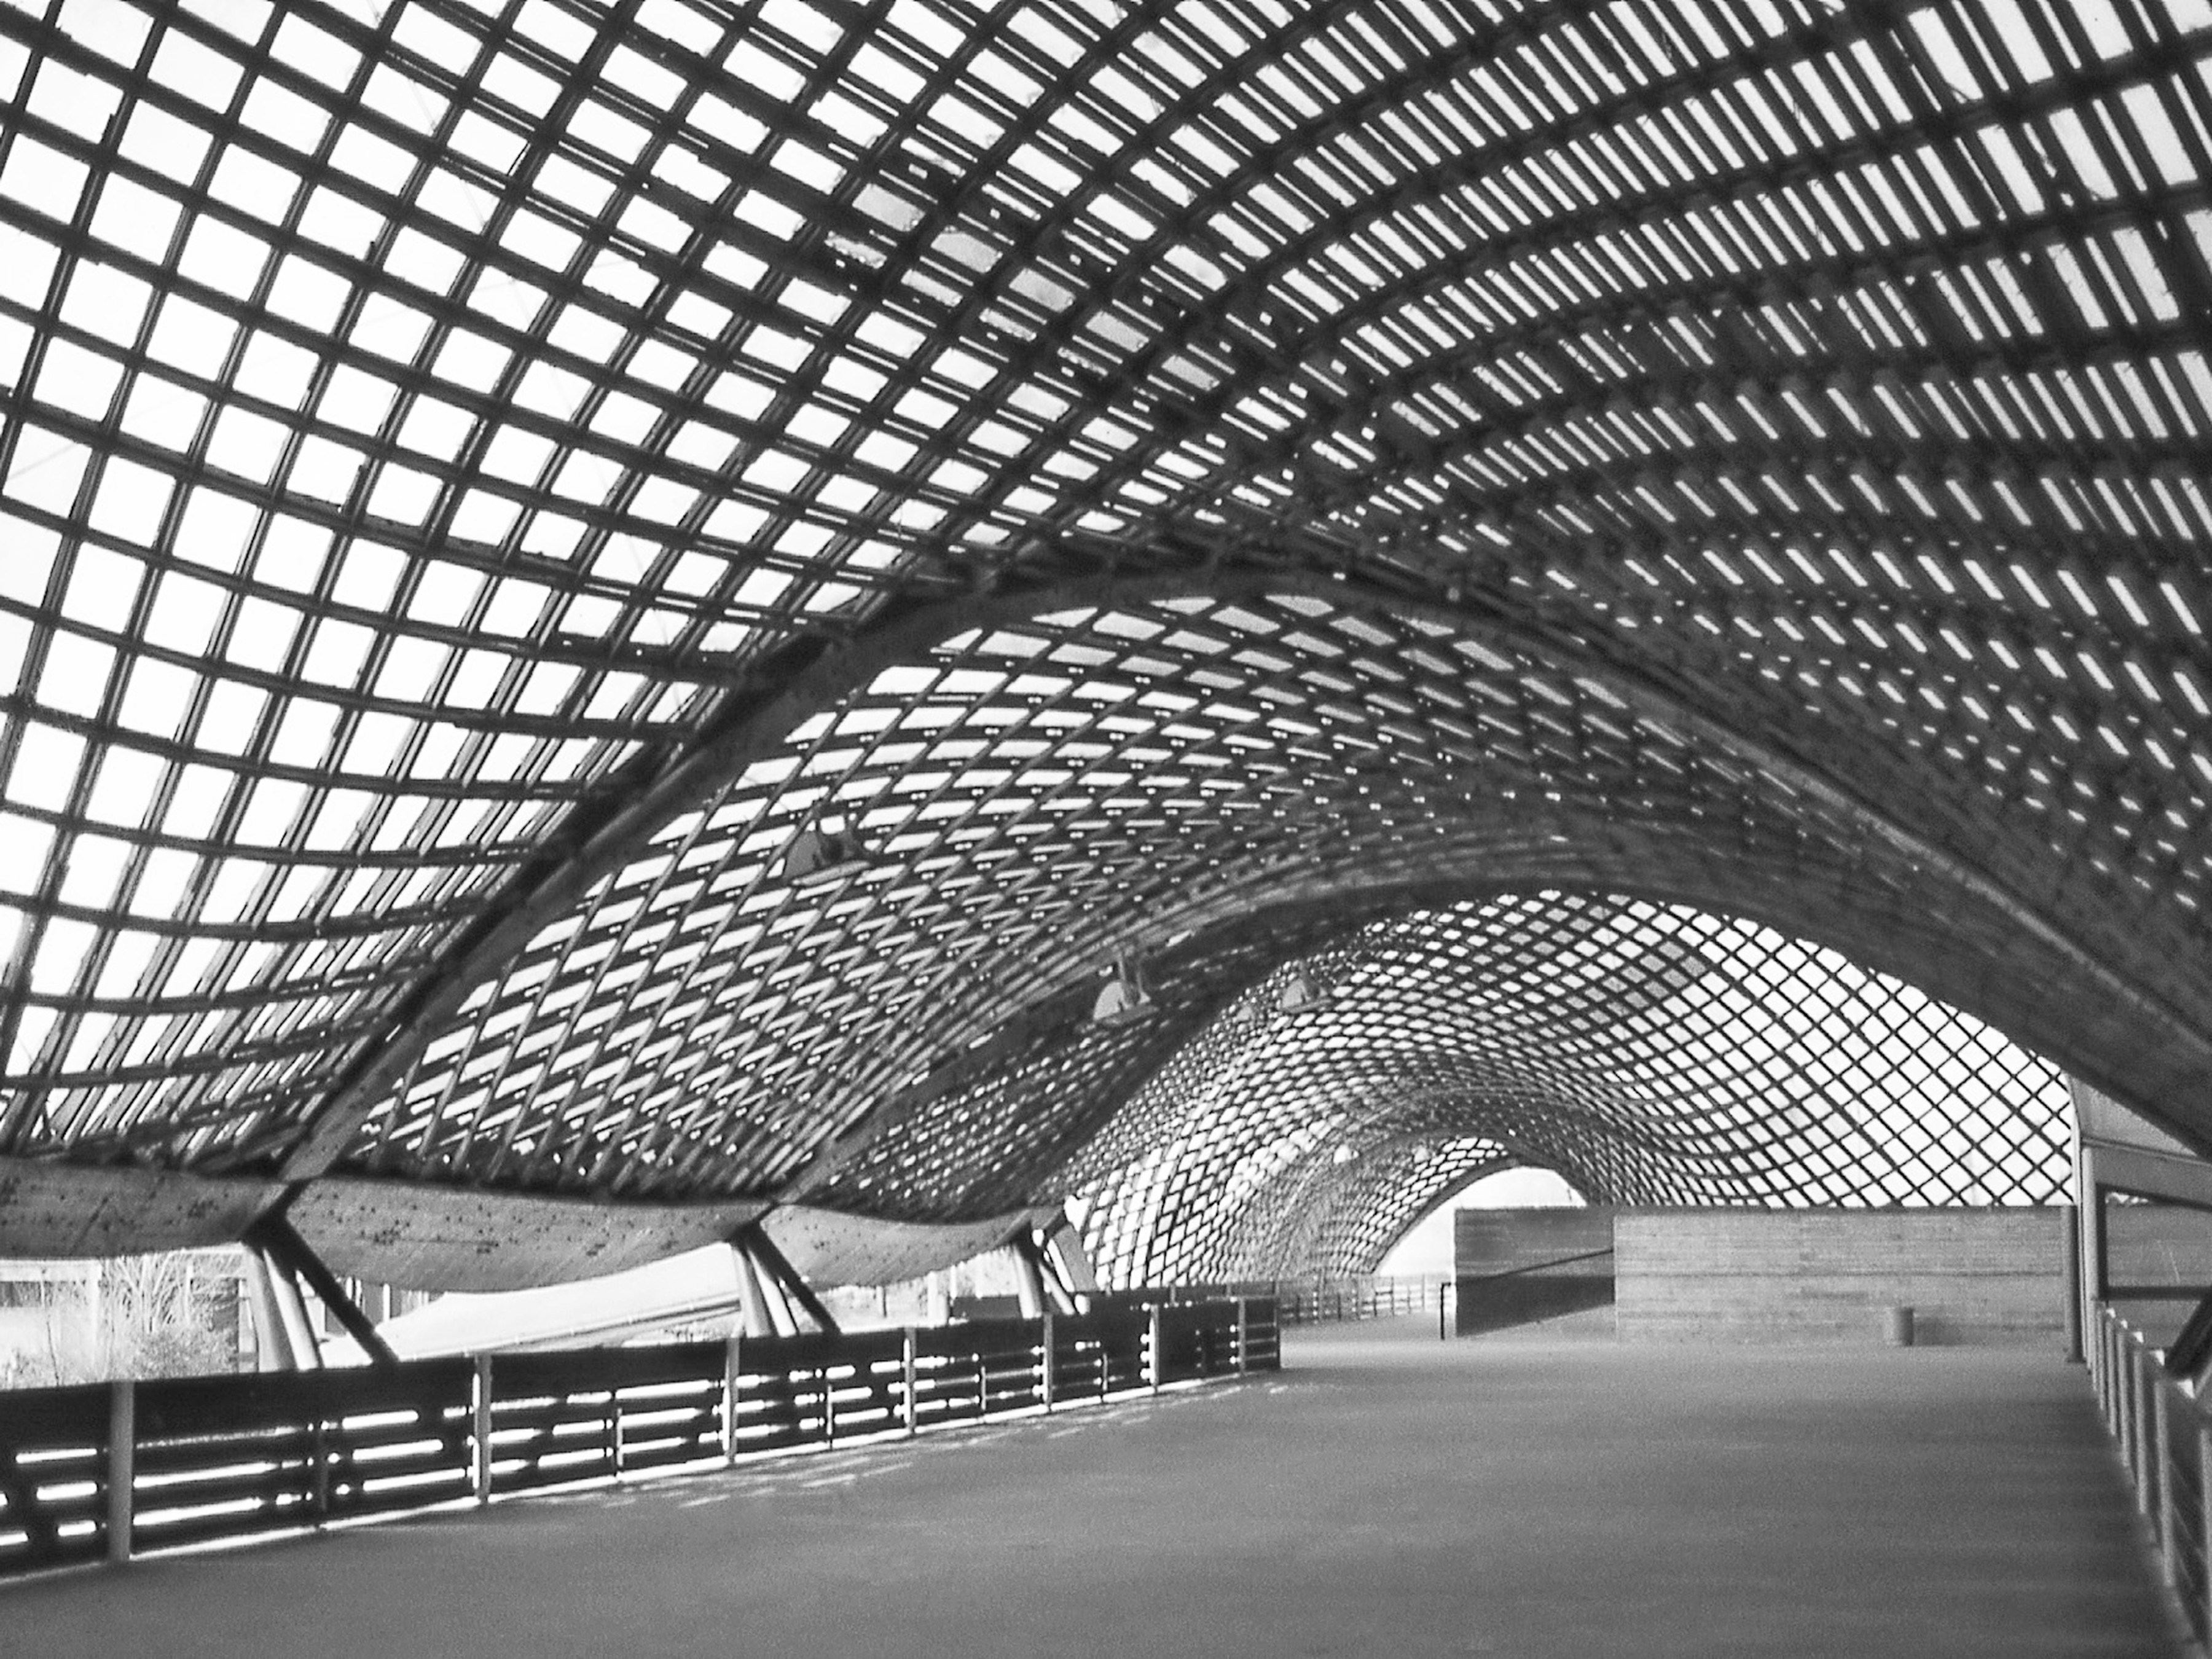
\includegraphics[width=0.48\textwidth]{mannheim_b.jpg}\label{fig:mannheim_b}} \\
		%
		\subfloat[][Downland (2002).]{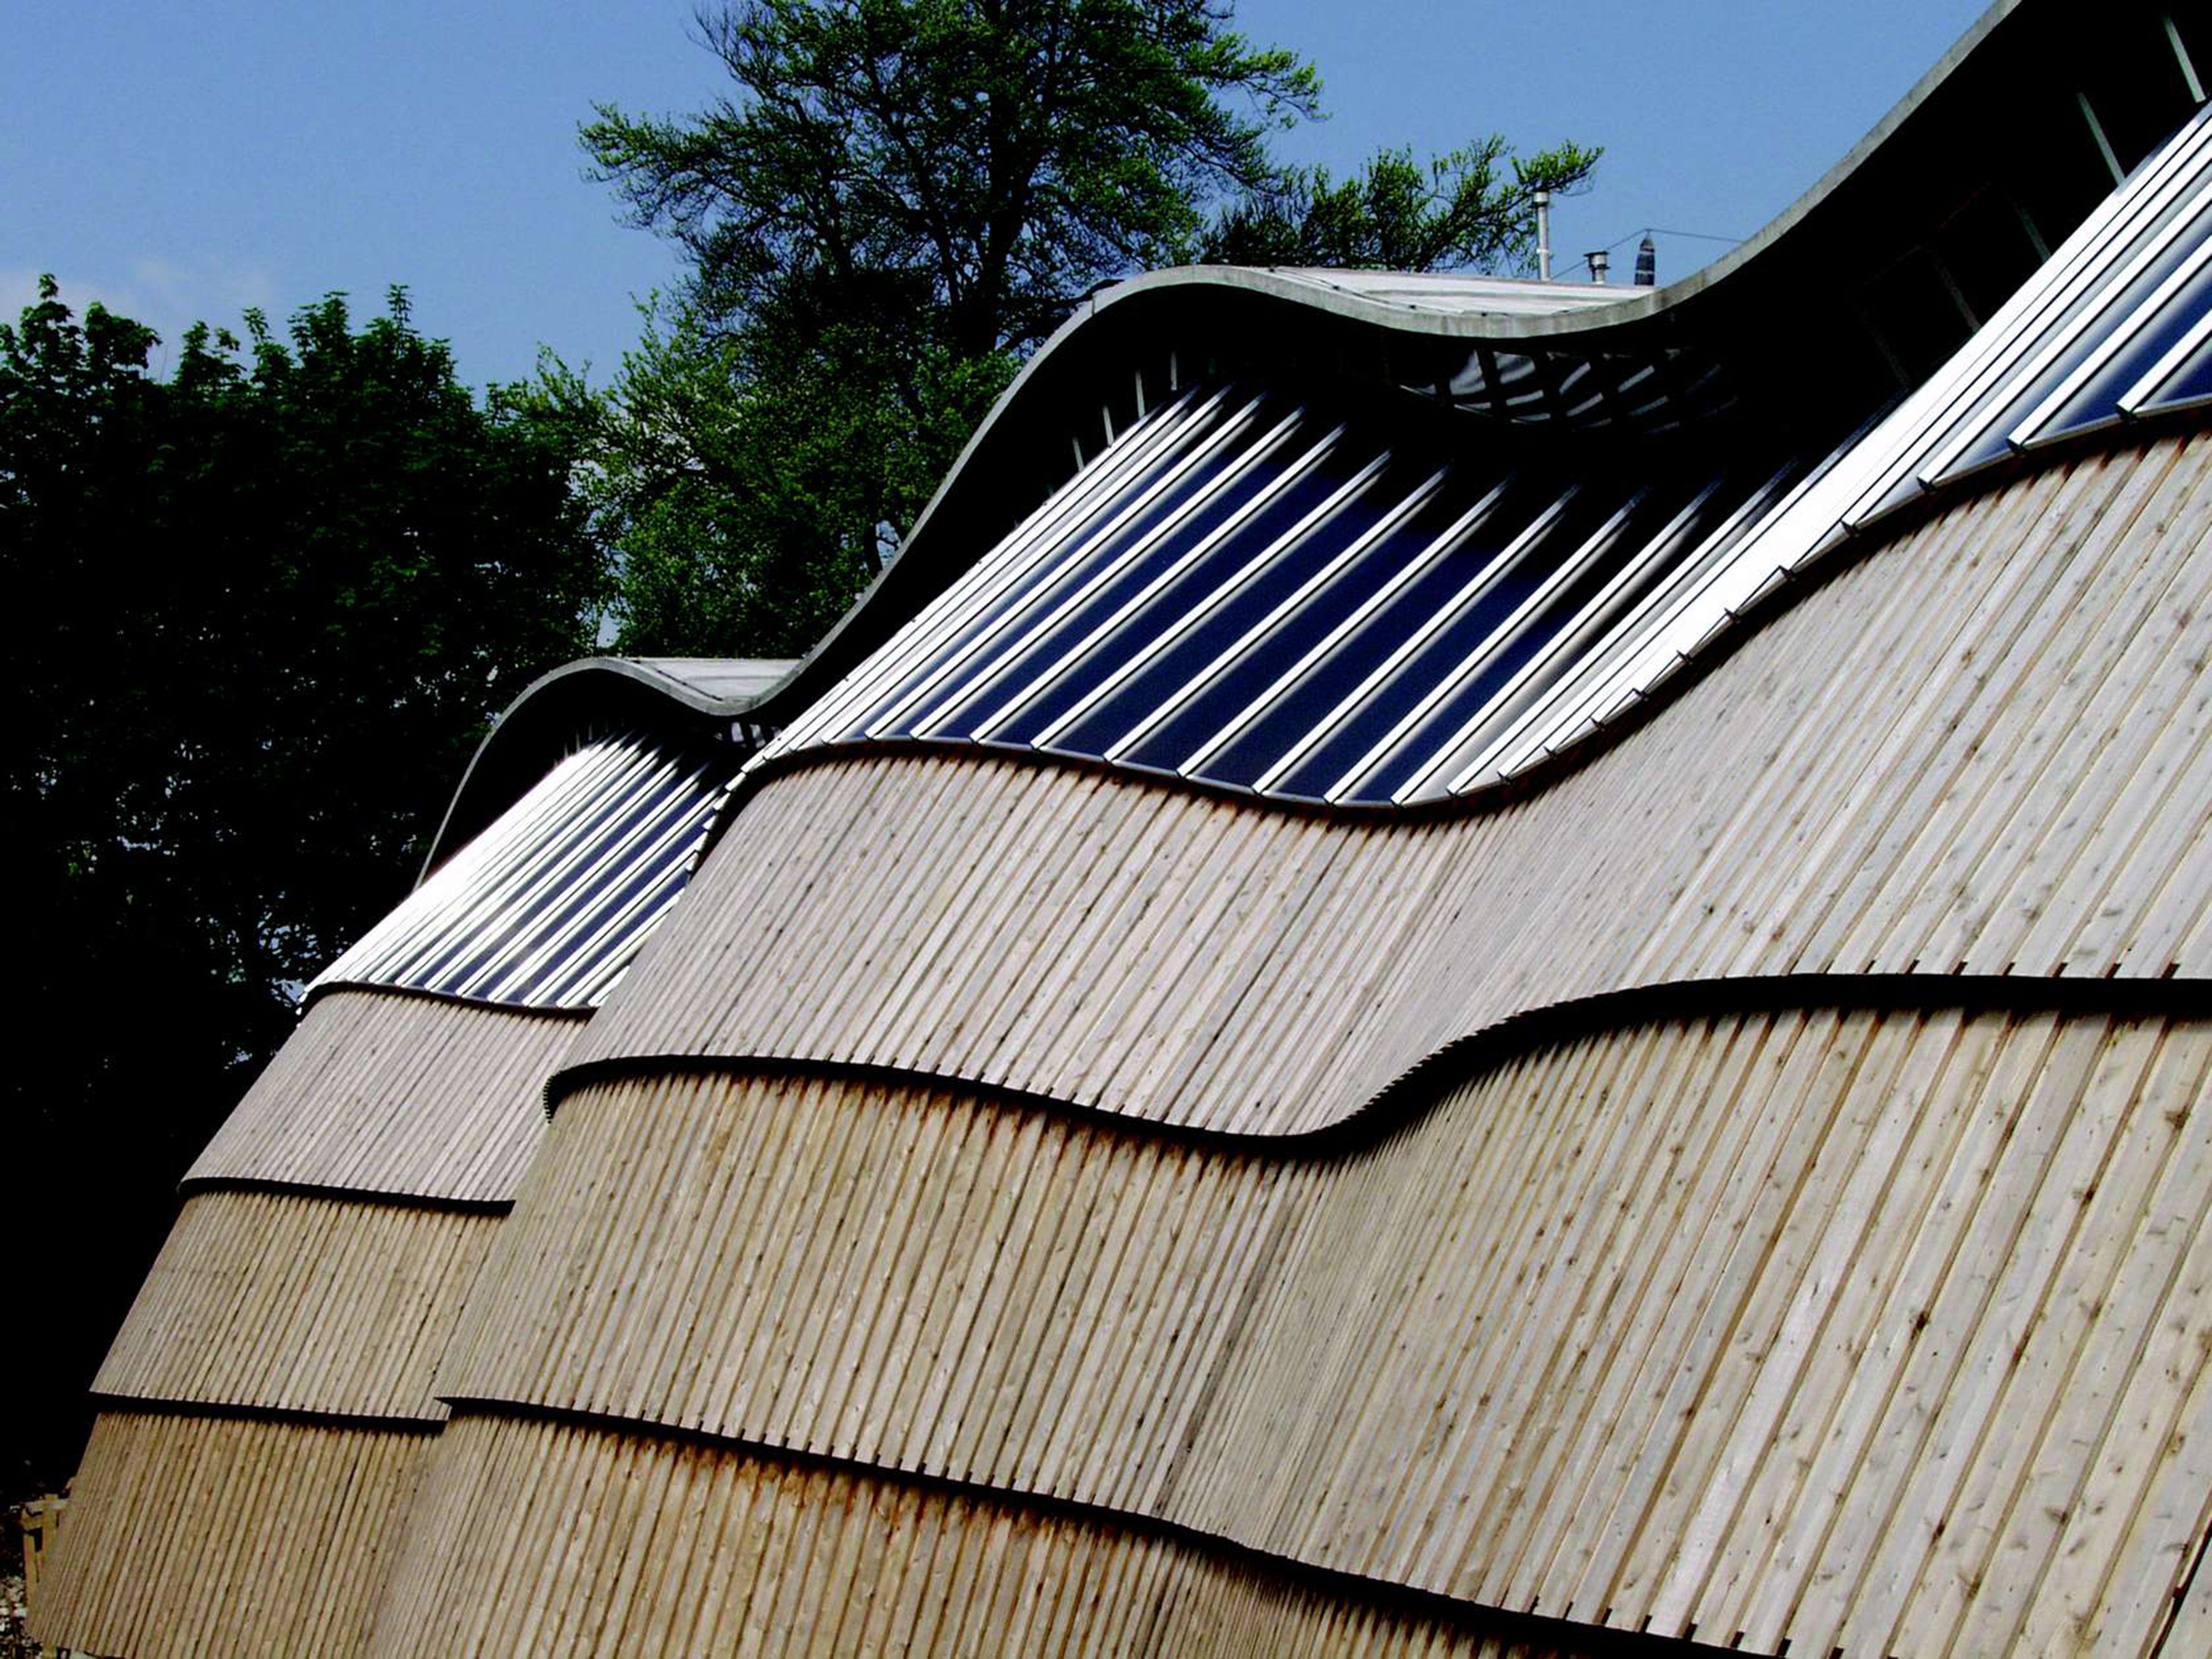
\includegraphics[width=0.48\textwidth]{downland_a.jpg}\label{fig:downland_a}}
		\hspace*{\fill}
		\subfloat[][Downland (2002).]{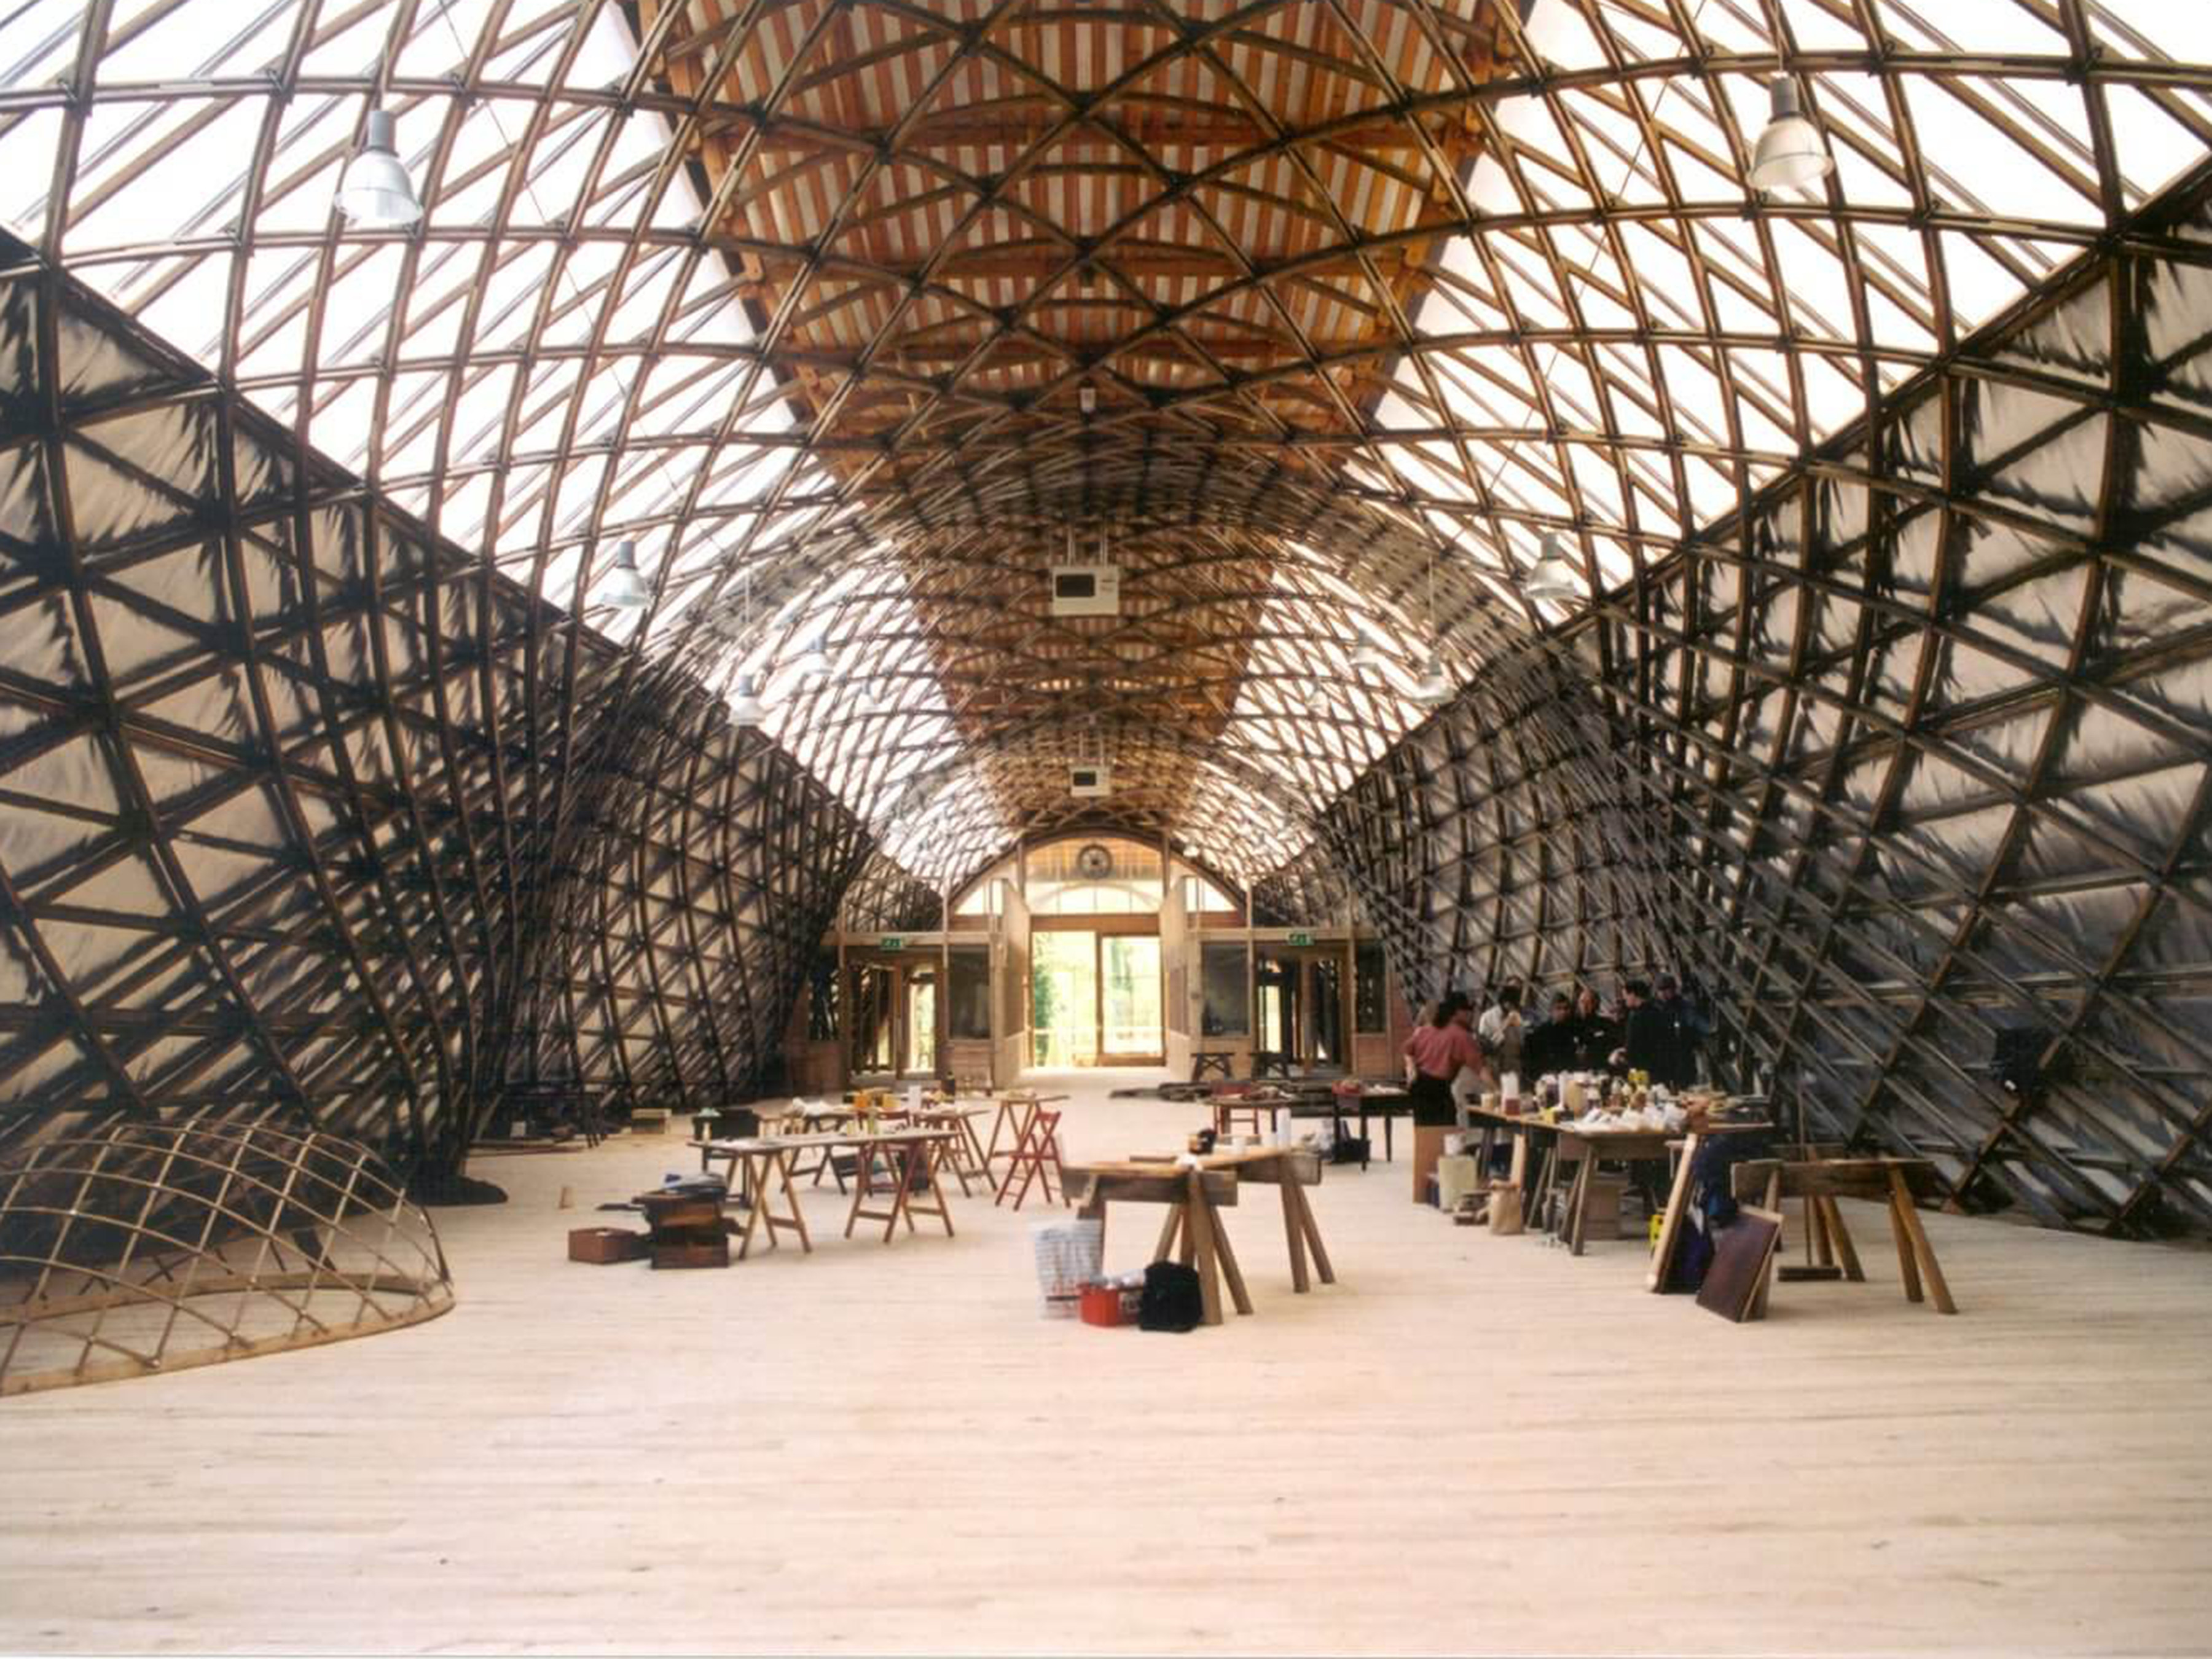
\includegraphics[width=0.48\textwidth]{downland_b.jpg}\label{fig:downland_b}} \\
		%
		\subfloat[][Savill (2006).]{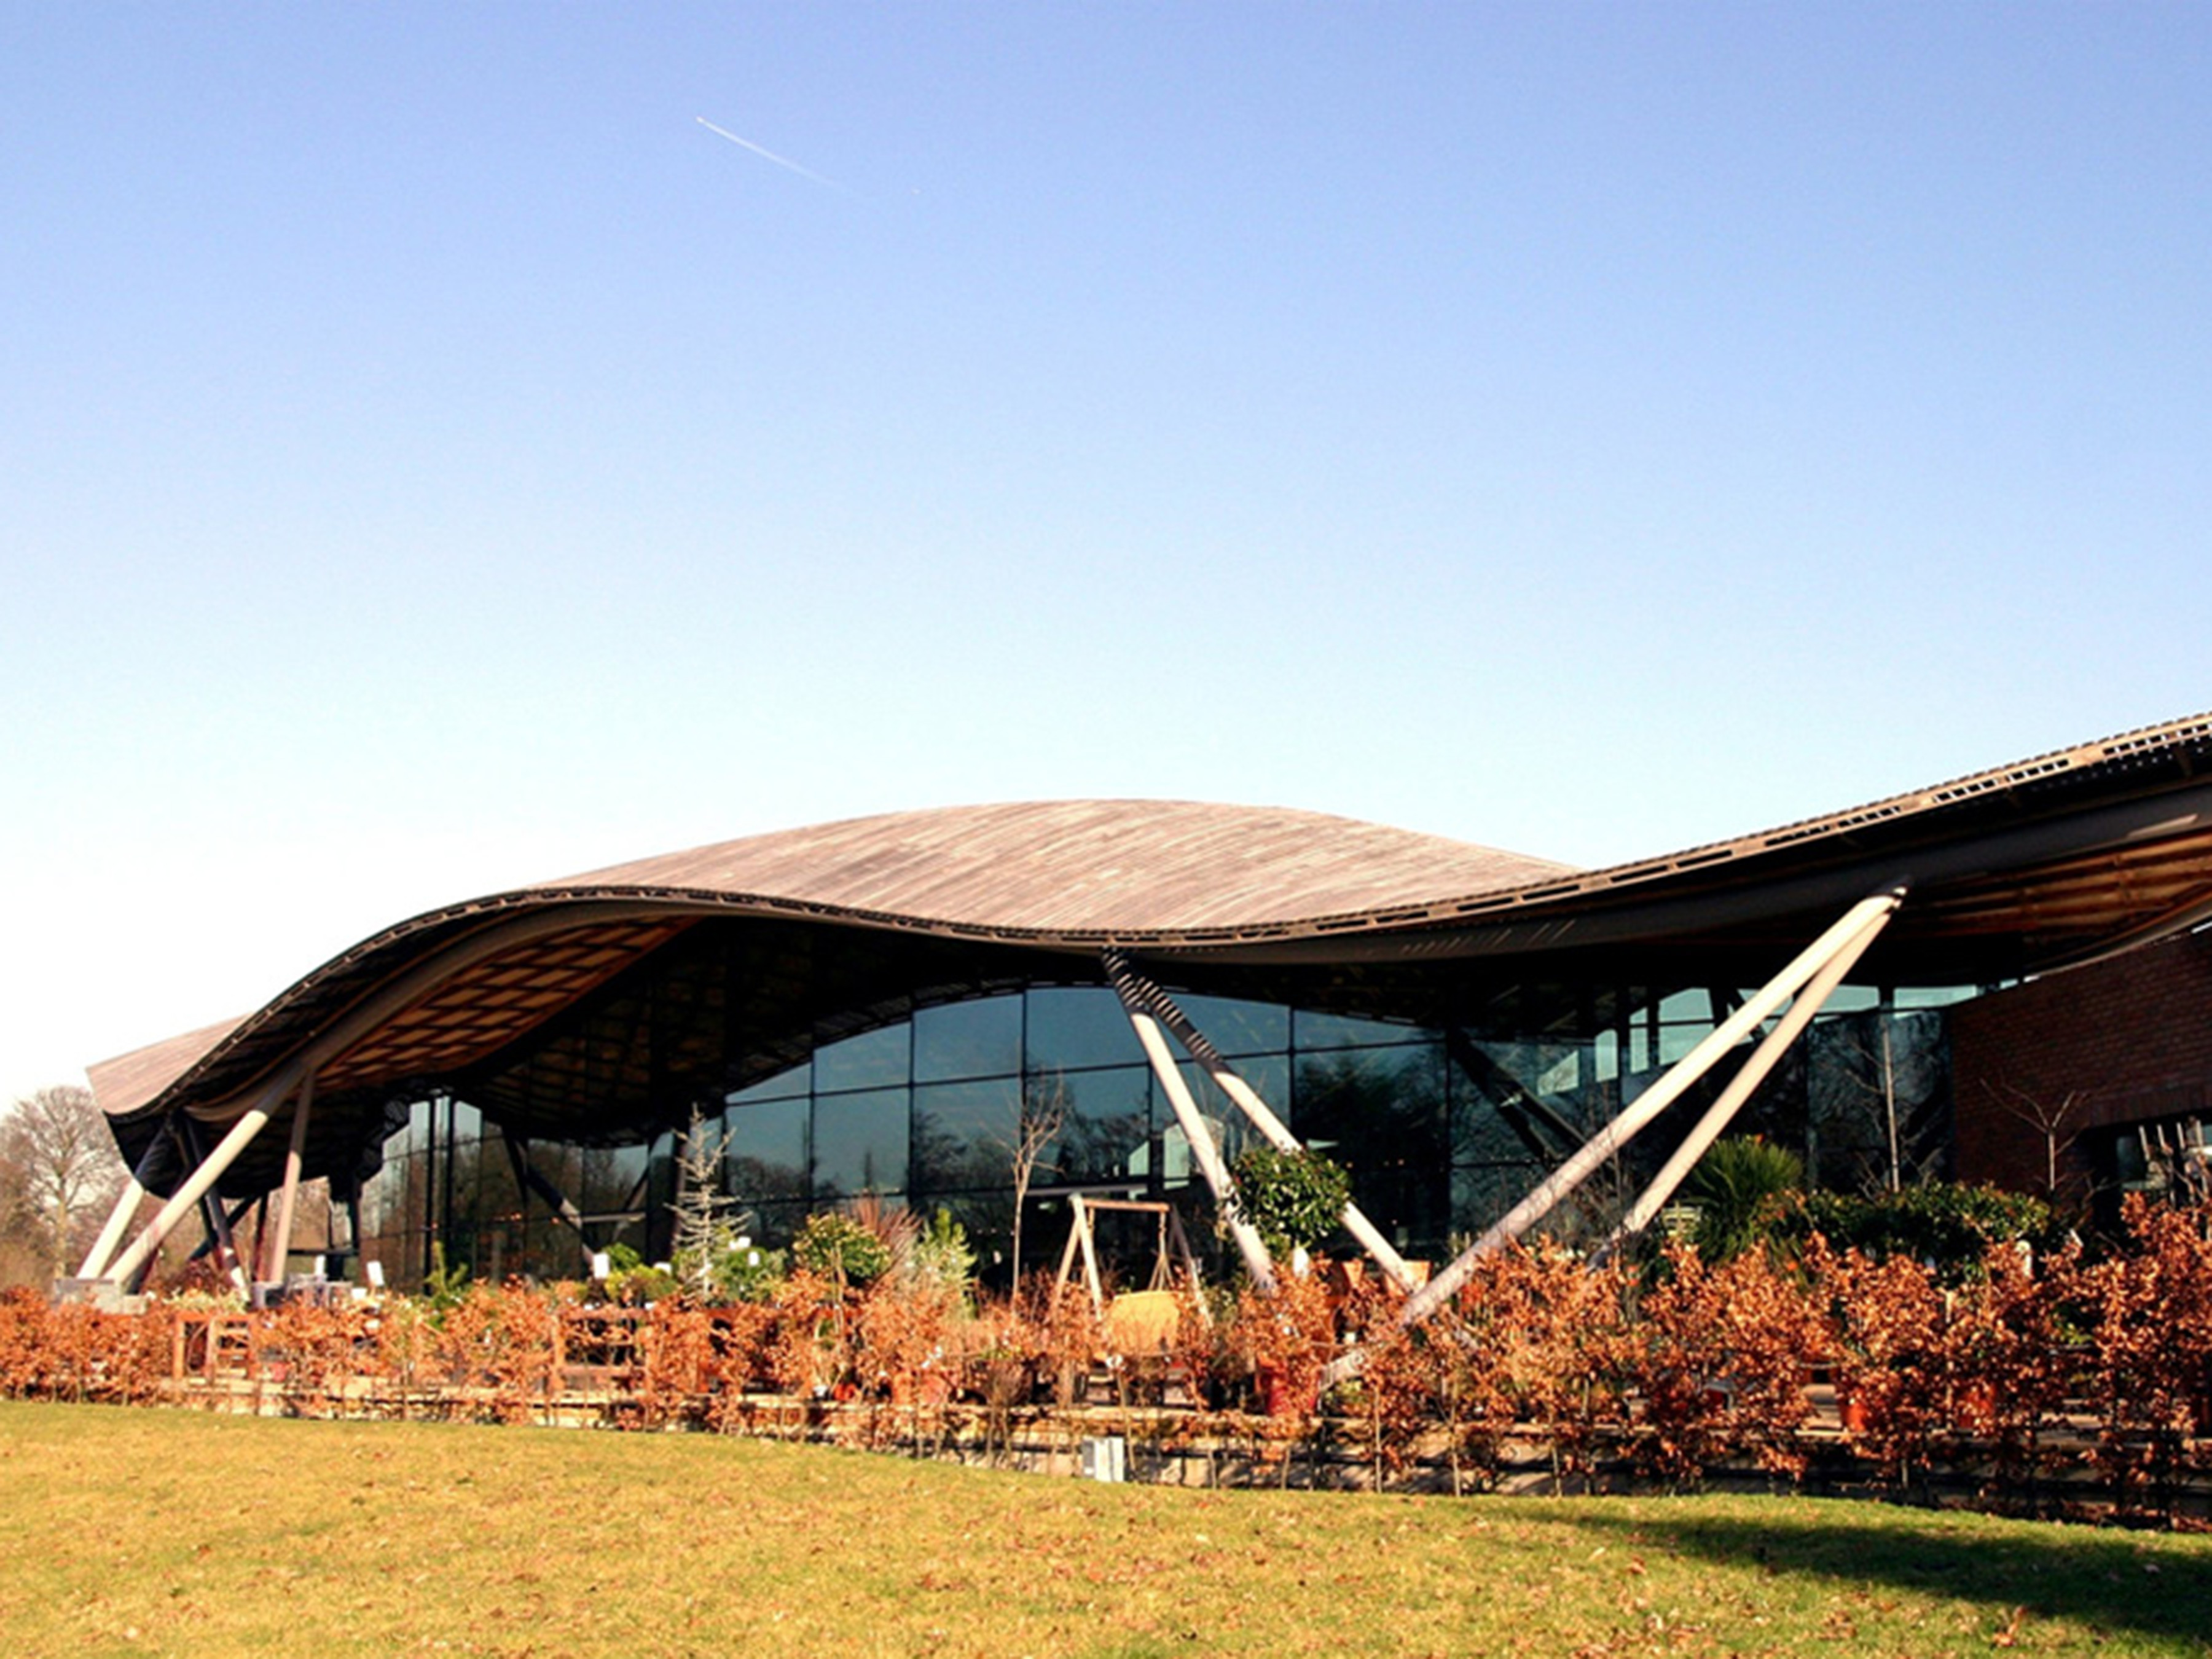
\includegraphics[width=0.48\textwidth]{savill_a.jpg}\label{fig:savill_a}}
		\hspace*{\fill}
		\subfloat[][Savill (2006).]{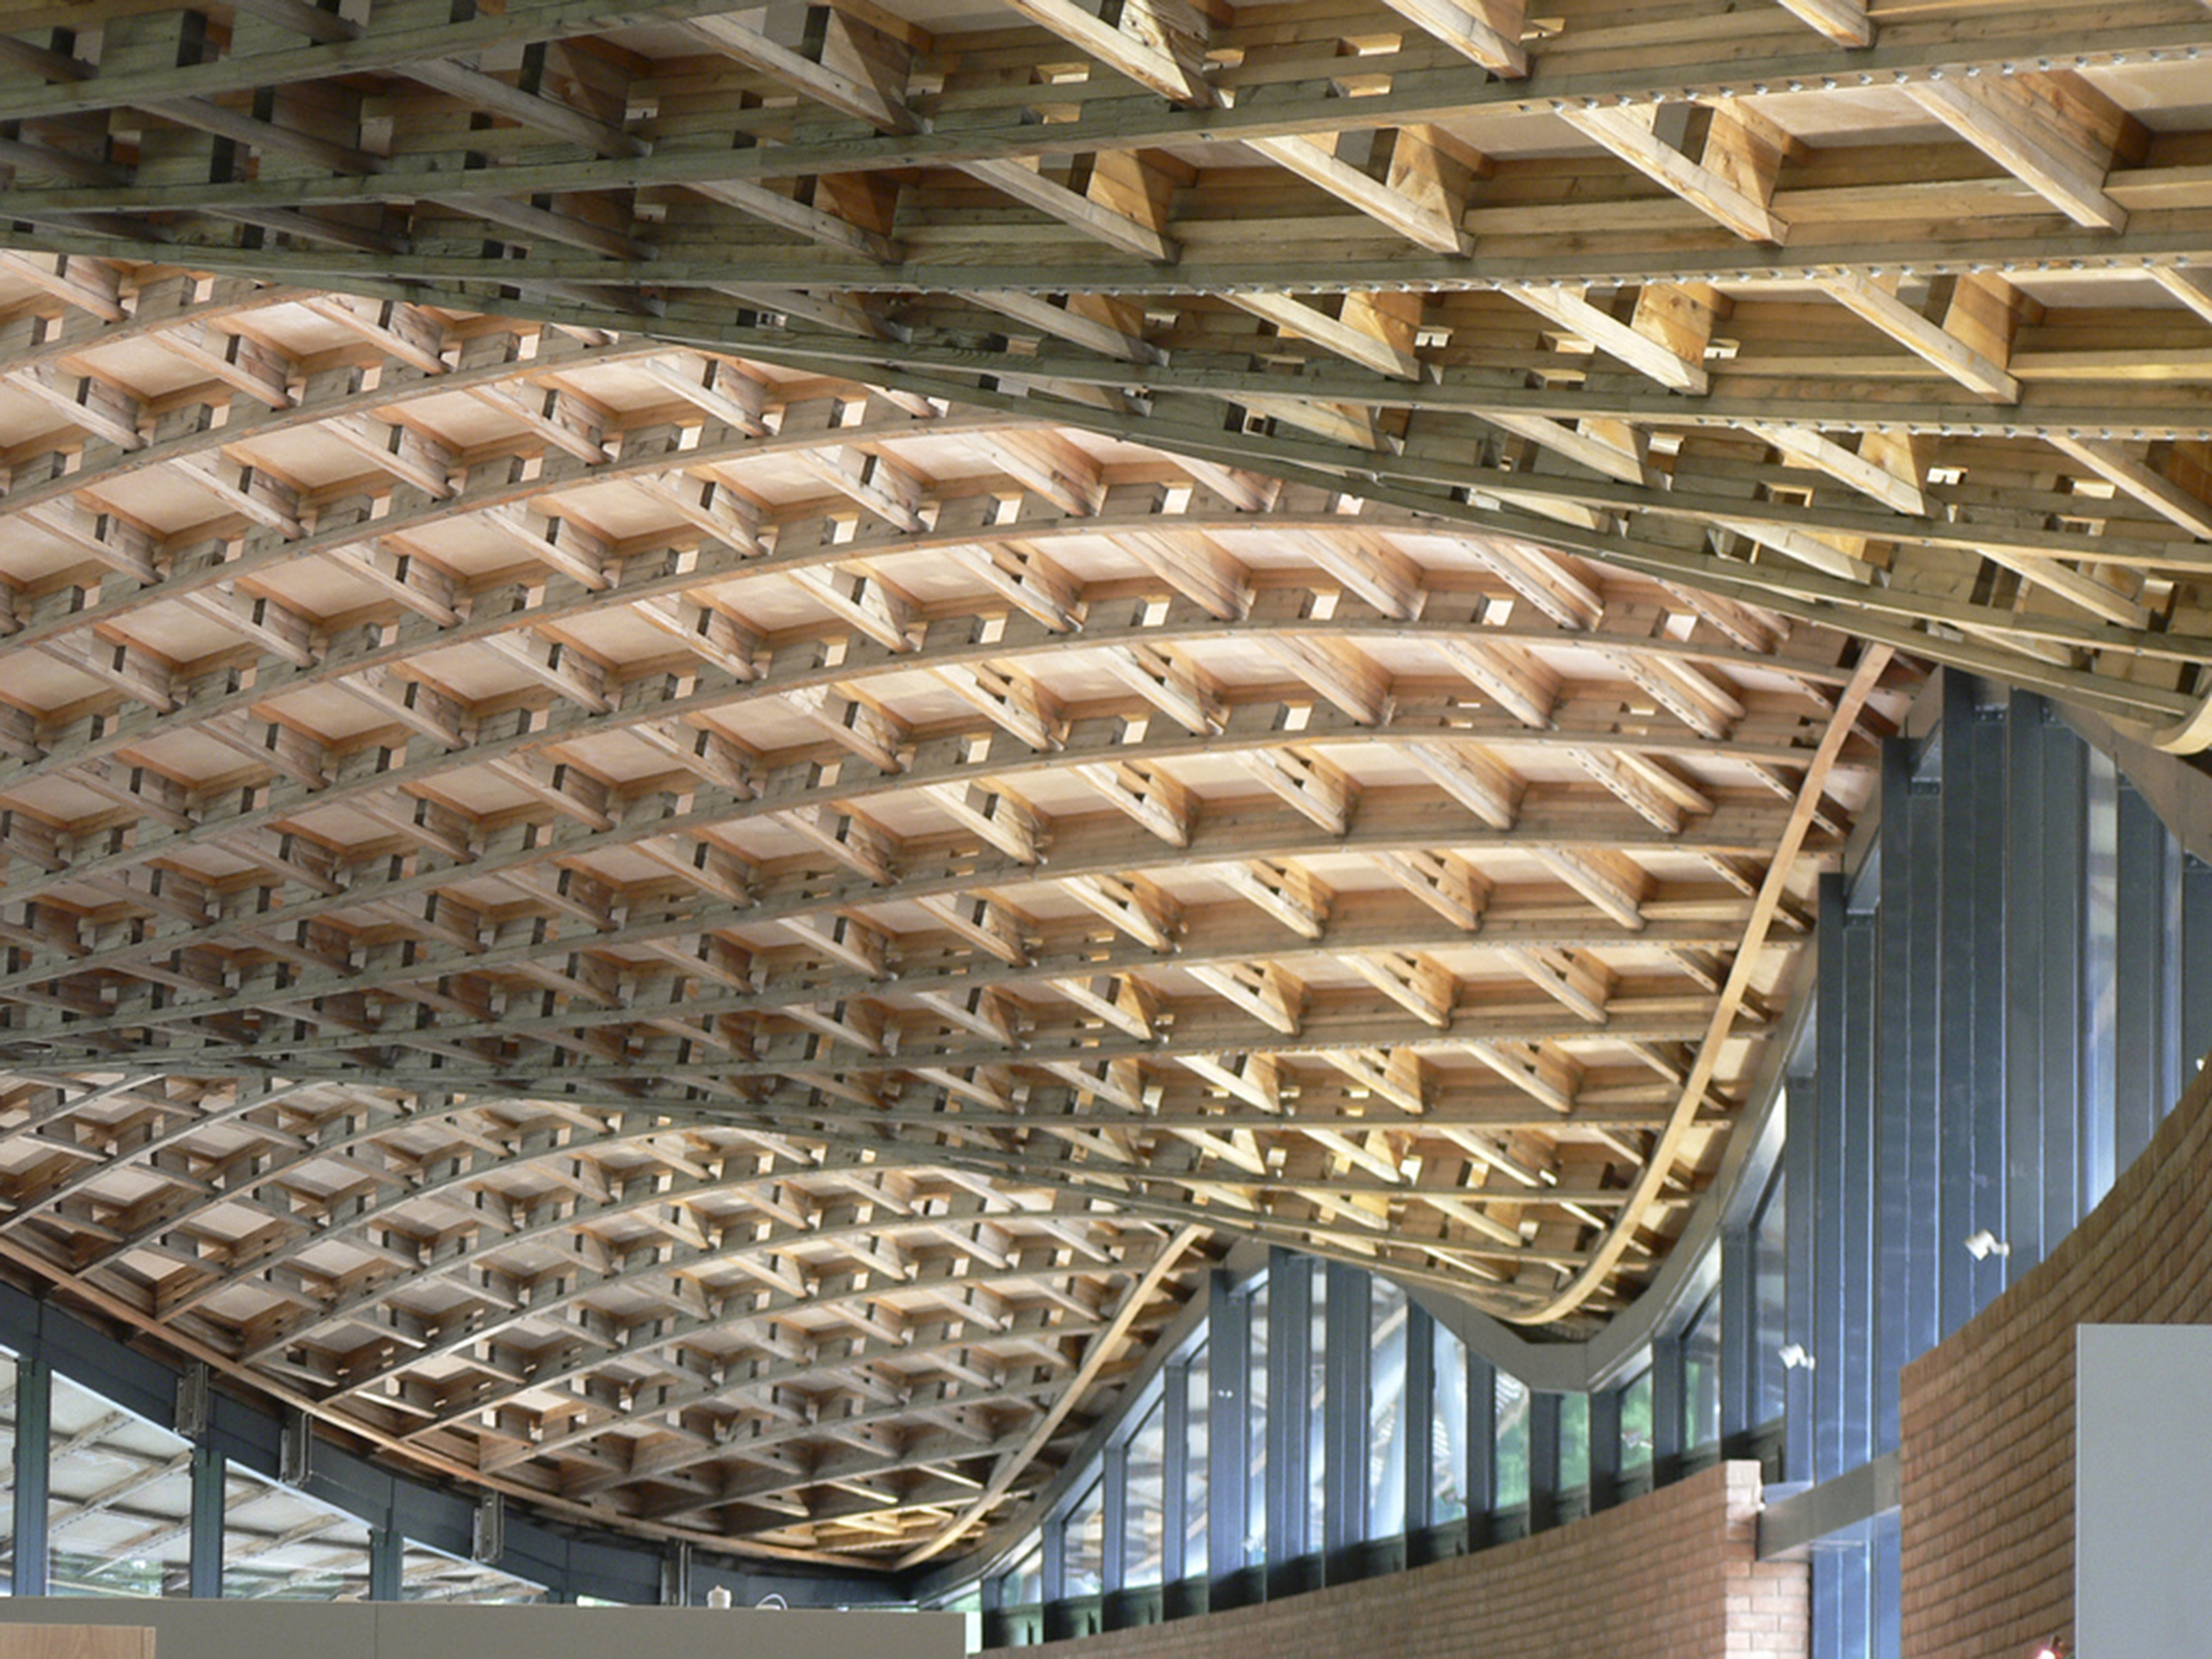
\includegraphics[width=0.48\textwidth]{savill_b.jpg}\label{fig:savill_b}}
		%
		\vspace{20pt}
		\caption{Major permanent projects of elastic wooden gridshells built since 1975.}
		\label{fig:projects}    
	\end{fullpage}
\end{figure}


\section{Elastic gridshells : revisiting Mannheim}


\section{Elastic gridshells : the benefits of composite materials}

Glass fiber reinforced polymer (GFRP) tubes are at the heart of the presented technology. They can favorably replace wood where both resistance and bending ability of the material is sought \cite{Douthe2010}. 

The tubes are made by pultrusion, \enquote{a continuous molding process whereby reinforcing fibers are saturated with a liquid polymer resin and then carefully formed and pulled through a heated die to form a part. Pultrusion results in straight constant cross section parts of virtually any shippable length}.\footnote{Video explaining the pultrusion process~: \url{https://www.youtube.com/watch?v=4MoHNZB5b_Y}} This process is very economic and its standardization guarantees very stable material and mechanical properties. It frees designers from the problem of joining wood pieces with finger joints to obtain long and continuous members and of wood durability.

\begin{figure}[h]
	\centering
		\captionsetup[subfloat]{captionskip=10pt}
		\subfloat[][Forum Café, Solidays (2011).]{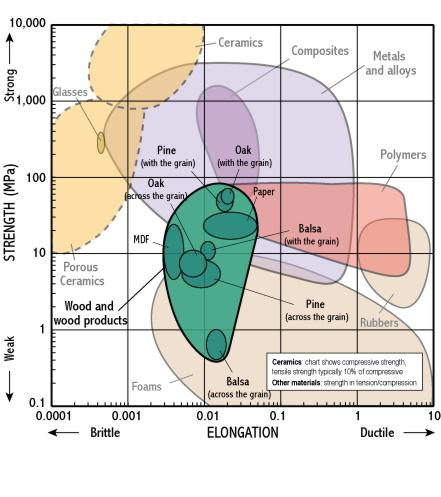
\includegraphics[width=0.6\textwidth]{ashby_woods.jpg}\label{fig:asby_co}}
		\\ \vspace{1cm}
		\subfloat[][Prototype (2007).]{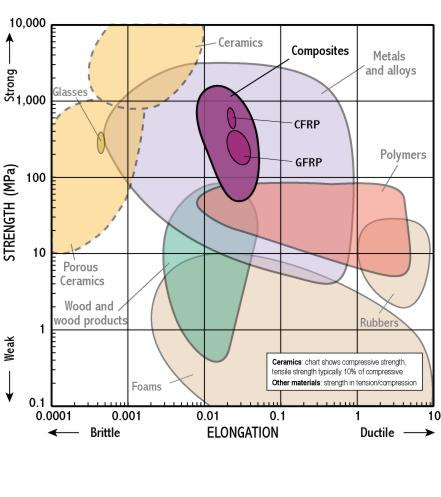
\includegraphics[width=0.6\textwidth]{ashby_composites.jpg}\label{fig:proto_a}}
		%
		\vspace{10pt}
		\caption{Prototypes and projects of GFRP elastic gridshells.}
		\label{fig:proto}    
\end{figure}

\section{Gridshells}

\subsection{Recent projects}
% ------------------------------------------

In 2000, Shigeru Ban innovated by shifting from wooden materials to cardboard for the construction of the Japan Pavilion at the Hanover Expo \cite{McQuaid2006}. More recently, with the development of numerical tools, two new projects were carried out: the wooden gridshells of Downland in 2002 (Weald and Downland Gridshell, Chichester, UK) \cite{Harris2003} and Savill in 2006 (Savill Garden Gridshell, Wick Ln, UK) \cite{Harris2008}. The principles of these projects are similar to that of Mannheim; however, new construction methods were used for the newer gridshells.

The first research works on elastic gridshells are attributed to Frei Otto, founder of the \emph{Institute for Lightweight Structures} (IL, Stuttgart, Germany). Probably one of his first elastic gridshell was built in 1962 with students at Berkley, USA, and was made with steel rods and not wooden elements. During the 60's, he built several experimental structures including one at Essen in 1962 and two at Montreal in 1967 \cite{Liddell2015}. In 1975 he completed the famous Mannheim Multihalle, a wooden shell of \SI{7500 }{m^2}, in collaboration with the engineer Edmund Happold \cite{Happold1975,Otto1976}. This project is generally regarded as the starting point of this new concept.

In 2000, Shigeru Ban innovated by shifting from wooden materials to cardboard for the construction of the Japan Pavilion at the Hanover Expo \cite{McQuaid2006}. More recently, with the development of numerical tools, new projects were carried out~: the wooden gridshells of Downland, UK, in 2002 \cite{Harris2003} and Savill, UK, in 2006 \cite{Harris2008}. The principles of these projects are similar to that of Mannheim. However, new construction methods were used for the newer gridshells. The flat lattice of the Downland gridshell was built on a modular scaffold platform, which height was altered progressively to deform the lattice. The grid was braced by a third direction of laths. The lattice of the Savill gridshell was built on a fixed scaffold platform. Small jacks where used to deform the lattice, pushing from below. The grid was then braced with plywood panels, which also served as the first cladding layer. 

The Orangery roof at Chiddingstone Castle is a smaller gridshell built in 2006. The lattice is very similar to the one employed in Downland. But this time the grid is braced with a diagonal cable network and the cladding is made of triangular glass panels (the first of this kind). To this end, the steel connection includes a cable clamping system and is equipped with a threaded hole to accept fixing parts for the glazing.




\subsection{Recent developments}
% ------------------------------------------
Based on this groundwork, the Navier laboratory has developed a research program on gridshells for the last decade, focusing on both the use of new materials and the development of more efficient numerical methods \cite{Douthe2007}. These developments have been validated by the construction of two prototypes (Figures \ref{fig:4}a and \ref{fig:4}b) whose areas were about 150 m\textsuperscript{2}.


In 2011, the laboratory used its expert knowledge for a large-scale project \cite{Baverel2012}, the forum of the Solidays festival (\autoref{fig:4}c). This achievement, built by voluntary workers, has been the first composite material gridshell to house public.

In 2012, the context is favorable for a new achievement named \emph{"Temporary Cathedral of Créteil"}. Although this gridshell has an area very similar to the Solidays one, the project raised new challenges, in particular the challenge of reliability. Indeed, its period of use is at least two years. Additionally, the skills coming from T/E/S/S company made possible important developments such as for doors, lacing edge beam, anchorages and sleeves.

Unlike the two first prototypes, the gridshells built for Solidays and at Créteil are based on a new approach regarding shape-structure relationship. Indeed, thanks to a numerical tool performing the compass method, the geometry of the object is no longer defined as the reversal of a hanging net – in this case, only the flat geometry could be mastered \cite{Addis2013} – but now the flat geometry is straight deducted from the one proposed by the architect.
This new approach opens up new architectural horizons, making possible the exploration of new shapes for gridshells.

The Faraday Pavilion : \cite{Nicholas2013}
The Pishwanton / lothian : \cite{Pishwanton2003}
The laboratory Navier tested various numerical methods to generate such grids \cite{Bouhaya2009}
Masson :  \cite{Masson2017}.
\begin{figure}[t]
	\centering
		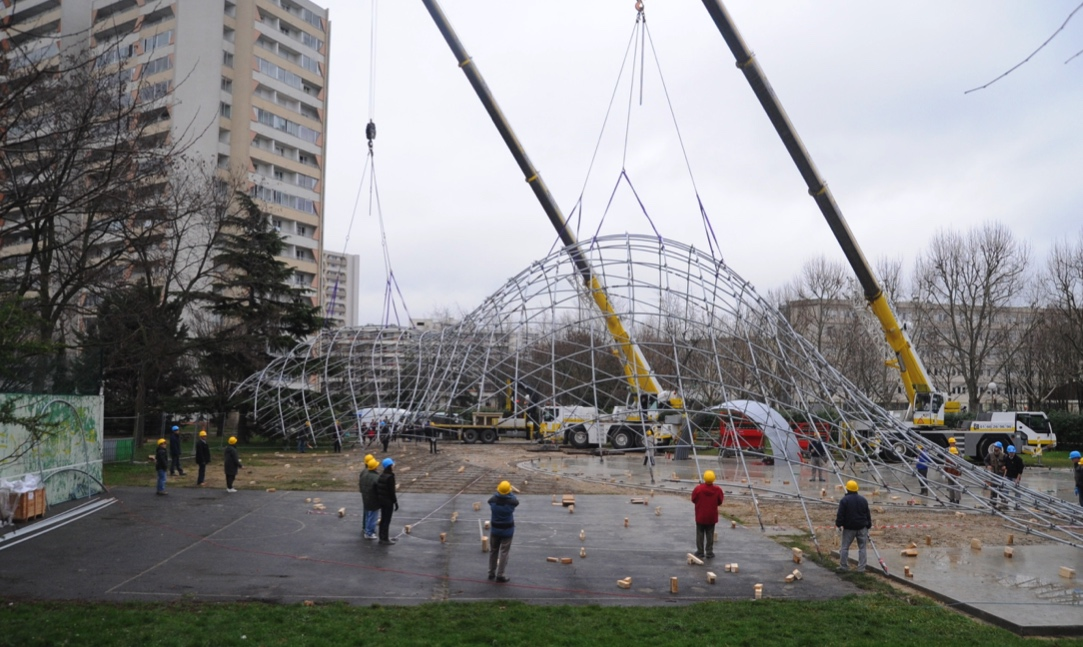
\includegraphics[width=\textwidth]{image6}
	\caption{Erection of the primary grid by two cranes}
	\label{fig:5}
\end{figure}



\subsection{Gridshell in composite material}
% ------------------------------------------

The benefits of GFRP gridshells have been covered previously. We just recall the main aspects.

The gridshells built in composite material, being at the heart of this paper, are consistent with the framework defined previously, that is to say :


Glass fiber reinforced polymer (GFRP) tubes are at the heart of the presented technology. They can favorably replace wood where both resistance and bending ability of the material is sought \cite{Douthe2010}. 

The tubes are made by pultrusion, \enquote{a continuous molding process whereby reinforcing fibers are saturated with a liquid polymer resin and then carefully formed and pulled through a heated die to form a part. Pultrusion results in straight constant cross section parts of virtually any shippable length}.\footnote{Video explaining the pultrusion process~: \url{https://www.youtube.com/watch?v=4MoHNZB5b_Y}} This process is very economic and its standardization guarantees very stable material and mechanical properties. It frees designers from the problem of joining wood pieces with finger joints to obtain long and continuous members and of wood durability. 


\subsubsection{Structural Typology}
% ------------------------------------------
Their mechanical behaviour is very similar to the one of real shells even if the material is discrete and located in a grid more or less open. In spite of that, gridshells benefit from the same advantages as the ones showed by an eggshell : they can cross large span using a low amount of material. Their stiffness is mainly linked to their double-curved shape.


\subsubsection{Material Flexibility for Structural Rigidity}
% ------------------------------------------
In this field of application, composite materials like glass fibre reinforced polymer (GFRP) could favourably replace wood, where both resistance and bending ability of the material is sought \cite{Douthe2010}. The stiffness of the structure does not derive from the intrinsic material rigidity but principally from its geometric curvature. Ideally, the composite profiles are produced by pultrusion, an economic continuous moulded process. The standardization of the process guaranties very stable material and mechanical properties. It frees designers from the painful problematic of wood joining and wood durability. The characterization of this material is presented further in the paper.


\subsubsection{Erection Process}
% ------------------------------------------
Usually, the grid morphology is not trivial and leads to design numerous costly and complex joints. To overcome this issue, an original and innovative erection process was developed that takes advantage of the flexibility inherent to slender elements. A regular planar grid made of long continuous linear members is built on the ground (\autoref{fig:6}a). The elements are pinned together so the grid has no in-plane shear stiffness and can accommodate large-scale deformations during erection. Then, the grid is bent elastically to its final shape (\autoref{fig:5}). Finally, the grid is frozen in the desired shape with a third layer of bracing members (\autoref{fig:6}b) and the structure becomes a shell.
\begin{figure}[t]
	\begin{minipage}[b]{.70\linewidth}
		\centering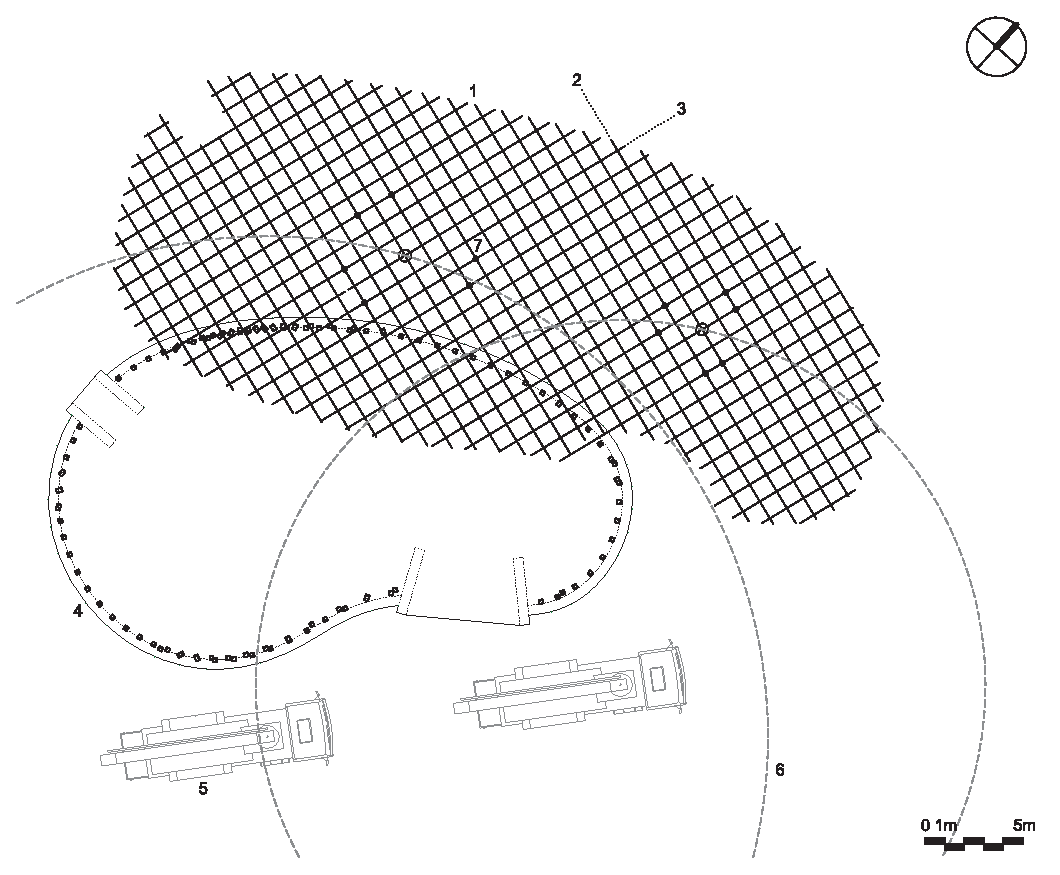
\includegraphics[width=0.95\textwidth]{image5}
	\end{minipage} \hfill
	\begin{minipage}[b]{.25\linewidth}
		\centering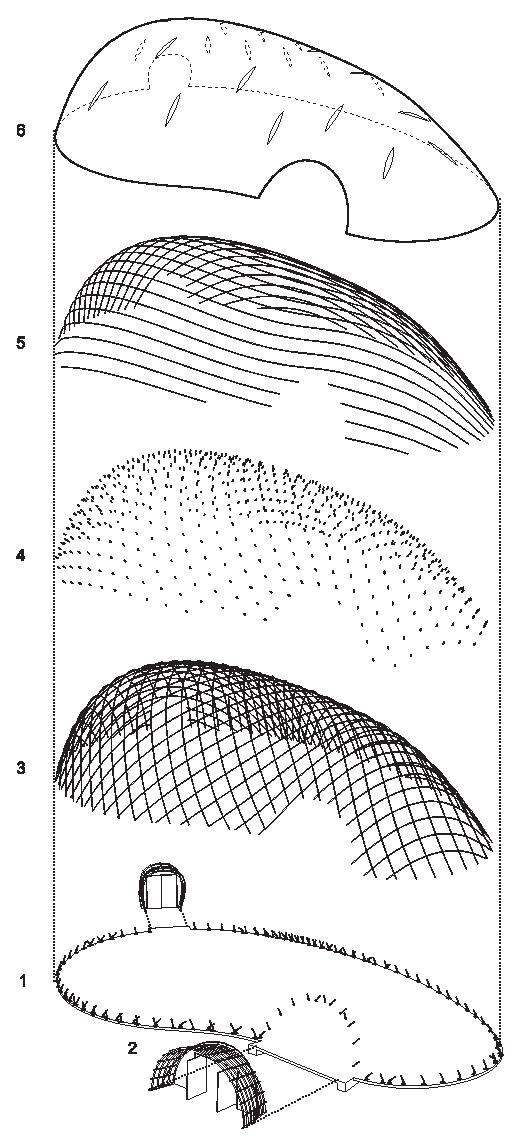
\includegraphics[width=0.93\textwidth]{image9}	
	\end{minipage}
	\vspace{0.5cm}
	\caption{Erection plan and construction stages}\label{fig:6}
\end{figure}

%\bibliographystyle{alpha}
%\bibliography{../library}

